% Options for packages loaded elsewhere
% Options for packages loaded elsewhere
\PassOptionsToPackage{unicode}{hyperref}
\PassOptionsToPackage{hyphens}{url}
\PassOptionsToPackage{dvipsnames,svgnames,x11names}{xcolor}
%
\documentclass[
  letterpaper,
  DIV=11,
  numbers=noendperiod,
  oneside]{scrreprt}
\usepackage{xcolor}
\usepackage[left=1in,marginparwidth=2.0666666666667in,textwidth=4.1333333333333in,marginparsep=0.3in]{geometry}
\usepackage{amsmath,amssymb}
\setcounter{secnumdepth}{5}
\usepackage{iftex}
\ifPDFTeX
  \usepackage[T1]{fontenc}
  \usepackage[utf8]{inputenc}
  \usepackage{textcomp} % provide euro and other symbols
\else % if luatex or xetex
  \usepackage{unicode-math} % this also loads fontspec
  \defaultfontfeatures{Scale=MatchLowercase}
  \defaultfontfeatures[\rmfamily]{Ligatures=TeX,Scale=1}
\fi
\usepackage{lmodern}
\ifPDFTeX\else
  % xetex/luatex font selection
\fi
% Use upquote if available, for straight quotes in verbatim environments
\IfFileExists{upquote.sty}{\usepackage{upquote}}{}
\IfFileExists{microtype.sty}{% use microtype if available
  \usepackage[]{microtype}
  \UseMicrotypeSet[protrusion]{basicmath} % disable protrusion for tt fonts
}{}
\makeatletter
\@ifundefined{KOMAClassName}{% if non-KOMA class
  \IfFileExists{parskip.sty}{%
    \usepackage{parskip}
  }{% else
    \setlength{\parindent}{0pt}
    \setlength{\parskip}{6pt plus 2pt minus 1pt}}
}{% if KOMA class
  \KOMAoptions{parskip=half}}
\makeatother
% Make \paragraph and \subparagraph free-standing
\makeatletter
\ifx\paragraph\undefined\else
  \let\oldparagraph\paragraph
  \renewcommand{\paragraph}{
    \@ifstar
      \xxxParagraphStar
      \xxxParagraphNoStar
  }
  \newcommand{\xxxParagraphStar}[1]{\oldparagraph*{#1}\mbox{}}
  \newcommand{\xxxParagraphNoStar}[1]{\oldparagraph{#1}\mbox{}}
\fi
\ifx\subparagraph\undefined\else
  \let\oldsubparagraph\subparagraph
  \renewcommand{\subparagraph}{
    \@ifstar
      \xxxSubParagraphStar
      \xxxSubParagraphNoStar
  }
  \newcommand{\xxxSubParagraphStar}[1]{\oldsubparagraph*{#1}\mbox{}}
  \newcommand{\xxxSubParagraphNoStar}[1]{\oldsubparagraph{#1}\mbox{}}
\fi
\makeatother
\usepackage{fancyvrb}

\usepackage{color}
\usepackage{fancyvrb}
\newcommand{\VerbBar}{|}
\newcommand{\VERB}{\Verb[commandchars=\\\{\}]}
\DefineVerbatimEnvironment{Highlighting}{Verbatim}{commandchars=\\\{\}}
% Add ',fontsize=\small' for more characters per line
\usepackage{framed}
\definecolor{shadecolor}{RGB}{241,243,245}
\newenvironment{Shaded}{\begin{snugshade}}{\end{snugshade}}
\newcommand{\AlertTok}[1]{\textcolor[rgb]{0.68,0.00,0.00}{#1}}
\newcommand{\AnnotationTok}[1]{\textcolor[rgb]{0.37,0.37,0.37}{#1}}
\newcommand{\AttributeTok}[1]{\textcolor[rgb]{0.40,0.45,0.13}{#1}}
\newcommand{\BaseNTok}[1]{\textcolor[rgb]{0.68,0.00,0.00}{#1}}
\newcommand{\BuiltInTok}[1]{\textcolor[rgb]{0.00,0.23,0.31}{#1}}
\newcommand{\CharTok}[1]{\textcolor[rgb]{0.13,0.47,0.30}{#1}}
\newcommand{\CommentTok}[1]{\textcolor[rgb]{0.37,0.37,0.37}{#1}}
\newcommand{\CommentVarTok}[1]{\textcolor[rgb]{0.37,0.37,0.37}{\textit{#1}}}
\newcommand{\ConstantTok}[1]{\textcolor[rgb]{0.56,0.35,0.01}{#1}}
\newcommand{\ControlFlowTok}[1]{\textcolor[rgb]{0.00,0.23,0.31}{\textbf{#1}}}
\newcommand{\DataTypeTok}[1]{\textcolor[rgb]{0.68,0.00,0.00}{#1}}
\newcommand{\DecValTok}[1]{\textcolor[rgb]{0.68,0.00,0.00}{#1}}
\newcommand{\DocumentationTok}[1]{\textcolor[rgb]{0.37,0.37,0.37}{\textit{#1}}}
\newcommand{\ErrorTok}[1]{\textcolor[rgb]{0.68,0.00,0.00}{#1}}
\newcommand{\ExtensionTok}[1]{\textcolor[rgb]{0.00,0.23,0.31}{#1}}
\newcommand{\FloatTok}[1]{\textcolor[rgb]{0.68,0.00,0.00}{#1}}
\newcommand{\FunctionTok}[1]{\textcolor[rgb]{0.28,0.35,0.67}{#1}}
\newcommand{\ImportTok}[1]{\textcolor[rgb]{0.00,0.46,0.62}{#1}}
\newcommand{\InformationTok}[1]{\textcolor[rgb]{0.37,0.37,0.37}{#1}}
\newcommand{\KeywordTok}[1]{\textcolor[rgb]{0.00,0.23,0.31}{\textbf{#1}}}
\newcommand{\NormalTok}[1]{\textcolor[rgb]{0.00,0.23,0.31}{#1}}
\newcommand{\OperatorTok}[1]{\textcolor[rgb]{0.37,0.37,0.37}{#1}}
\newcommand{\OtherTok}[1]{\textcolor[rgb]{0.00,0.23,0.31}{#1}}
\newcommand{\PreprocessorTok}[1]{\textcolor[rgb]{0.68,0.00,0.00}{#1}}
\newcommand{\RegionMarkerTok}[1]{\textcolor[rgb]{0.00,0.23,0.31}{#1}}
\newcommand{\SpecialCharTok}[1]{\textcolor[rgb]{0.37,0.37,0.37}{#1}}
\newcommand{\SpecialStringTok}[1]{\textcolor[rgb]{0.13,0.47,0.30}{#1}}
\newcommand{\StringTok}[1]{\textcolor[rgb]{0.13,0.47,0.30}{#1}}
\newcommand{\VariableTok}[1]{\textcolor[rgb]{0.07,0.07,0.07}{#1}}
\newcommand{\VerbatimStringTok}[1]{\textcolor[rgb]{0.13,0.47,0.30}{#1}}
\newcommand{\WarningTok}[1]{\textcolor[rgb]{0.37,0.37,0.37}{\textit{#1}}}

\usepackage{longtable,booktabs,array}
\newcounter{none} % for unnumbered tables
\usepackage{multirow}
\usepackage{calc} % for calculating minipage widths
% Correct order of tables after \paragraph or \subparagraph
\usepackage{etoolbox}
\makeatletter
\patchcmd\longtable{\par}{\if@noskipsec\mbox{}\fi\par}{}{}
\makeatother
% Allow footnotes in longtable head/foot
\IfFileExists{footnotehyper.sty}{\usepackage{footnotehyper}}{\usepackage{footnote}}
\makesavenoteenv{longtable}
\usepackage{graphicx}
\makeatletter
\newsavebox\pandoc@box
\newcommand*\pandocbounded[1]{% scales image to fit in text height/width
  \sbox\pandoc@box{#1}%
  \Gscale@div\@tempa{\textheight}{\dimexpr\ht\pandoc@box+\dp\pandoc@box\relax}%
  \Gscale@div\@tempb{\linewidth}{\wd\pandoc@box}%
  \ifdim\@tempb\p@<\@tempa\p@\let\@tempa\@tempb\fi% select the smaller of both
  \ifdim\@tempa\p@<\p@\scalebox{\@tempa}{\usebox\pandoc@box}%
  \else\usebox{\pandoc@box}%
  \fi%
}
% Set default figure placement to htbp
\def\fps@figure{htbp}
\makeatother

\ifLuaTeX
  \usepackage{luacolor}
  \usepackage[soul]{lua-ul}
\else
  \usepackage{soul}
\fi

% definitions for citeproc citations
\NewDocumentCommand\citeproctext{}{}
\NewDocumentCommand\citeproc{mm}{%
  \begingroup\def\citeproctext{#2}\cite{#1}\endgroup}
\makeatletter
 % allow citations to break across lines
 \let\@cite@ofmt\@firstofone
 % avoid brackets around text for \cite:
 \def\@biblabel#1{}
 \def\@cite#1#2{{#1\if@tempswa , #2\fi}}
\makeatother
\newlength{\cslhangindent}
\setlength{\cslhangindent}{1.5em}
\newlength{\csllabelwidth}
\setlength{\csllabelwidth}{3em}
\newenvironment{CSLReferences}[2] % #1 hanging-indent, #2 entry-spacing
 {\begin{list}{}{%
  \setlength{\itemindent}{0pt}
  \setlength{\leftmargin}{0pt}
  \setlength{\parsep}{0pt}
  % turn on hanging indent if param 1 is 1
  \ifodd #1
   \setlength{\leftmargin}{\cslhangindent}
   \setlength{\itemindent}{-1\cslhangindent}
  \fi
  % set entry spacing
  \setlength{\itemsep}{#2\baselineskip}}}
 {\end{list}}
\usepackage{calc}
\newcommand{\CSLBlock}[1]{\hfill\break\parbox[t]{\linewidth}{\strut\ignorespaces#1\strut}}
\newcommand{\CSLLeftMargin}[1]{\parbox[t]{\csllabelwidth}{\strut#1\strut}}
\newcommand{\CSLRightInline}[1]{\parbox[t]{\linewidth - \csllabelwidth}{\strut#1\strut}}
\newcommand{\CSLIndent}[1]{\hspace{\cslhangindent}#1}



\setlength{\emergencystretch}{3em} % prevent overfull lines

\providecommand{\tightlist}{%
  \setlength{\itemsep}{0pt}\setlength{\parskip}{0pt}}



 


\KOMAoption{captions}{tableheading}
\makeatletter
\@ifpackageloaded{tcolorbox}{}{\usepackage[skins,breakable]{tcolorbox}}
\@ifpackageloaded{fontawesome5}{}{\usepackage{fontawesome5}}
\definecolor{quarto-callout-color}{HTML}{909090}
\definecolor{quarto-callout-note-color}{HTML}{0758E5}
\definecolor{quarto-callout-important-color}{HTML}{CC1914}
\definecolor{quarto-callout-warning-color}{HTML}{EB9113}
\definecolor{quarto-callout-tip-color}{HTML}{00A047}
\definecolor{quarto-callout-caution-color}{HTML}{FC5300}
\definecolor{quarto-callout-color-frame}{HTML}{acacac}
\definecolor{quarto-callout-note-color-frame}{HTML}{4582ec}
\definecolor{quarto-callout-important-color-frame}{HTML}{d9534f}
\definecolor{quarto-callout-warning-color-frame}{HTML}{f0ad4e}
\definecolor{quarto-callout-tip-color-frame}{HTML}{02b875}
\definecolor{quarto-callout-caution-color-frame}{HTML}{fd7e14}
\makeatother
\makeatletter
\@ifpackageloaded{bookmark}{}{\usepackage{bookmark}}
\makeatother
\makeatletter
\@ifpackageloaded{caption}{}{\usepackage{caption}}
\AtBeginDocument{%
\ifdefined\contentsname
  \renewcommand*\contentsname{Table of contents}
\else
  \newcommand\contentsname{Table of contents}
\fi
\ifdefined\listfigurename
  \renewcommand*\listfigurename{List of Figures}
\else
  \newcommand\listfigurename{List of Figures}
\fi
\ifdefined\listtablename
  \renewcommand*\listtablename{List of Tables}
\else
  \newcommand\listtablename{List of Tables}
\fi
\ifdefined\figurename
  \renewcommand*\figurename{Figure}
\else
  \newcommand\figurename{Figure}
\fi
\ifdefined\tablename
  \renewcommand*\tablename{Table}
\else
  \newcommand\tablename{Table}
\fi
}
\@ifpackageloaded{float}{}{\usepackage{float}}
\floatstyle{ruled}
\@ifundefined{c@chapter}{\newfloat{codelisting}{h}{lop}}{\newfloat{codelisting}{h}{lop}[chapter]}
\floatname{codelisting}{Listing}
\newcommand*\listoflistings{\listof{codelisting}{List of Listings}}
\makeatother
\makeatletter
\makeatother
\makeatletter
\@ifpackageloaded{caption}{}{\usepackage{caption}}
\@ifpackageloaded{subcaption}{}{\usepackage{subcaption}}
\makeatother
\makeatletter
\@ifpackageloaded{sidenotes}{}{\usepackage{sidenotes}}
\@ifpackageloaded{marginnote}{}{\usepackage{marginnote}}
\makeatother
\newcounter{quartocallouttipno}
\newcommand{\quartocallouttip}[1]{\refstepcounter{quartocallouttipno}\label{#1}}
\usepackage{bookmark}
\IfFileExists{xurl.sty}{\usepackage{xurl}}{} % add URL line breaks if available
\urlstyle{same}
\VerbatimFootnotes % allow verbatim text in footnotes
\hypersetup{
  pdftitle={AI QA Workbook},
  pdfauthor={Mario Winter},
  colorlinks=true,
  linkcolor={blue},
  filecolor={Maroon},
  citecolor={Blue},
  urlcolor={Blue},
  pdfcreator={LaTeX via pandoc}}


\title{AI QA Workbook}
\author{Mario Winter}
\date{2026-05-16}
\begin{document}
\maketitle

\renewcommand*\contentsname{Table of contents}
{
\setcounter{tocdepth}{2}
\tableofcontents
}

\bookmarksetup{startatroot}

\chapter*{Preface}\label{preface}
\addcontentsline{toc}{chapter}{Preface}

\markboth{Preface}{Preface}

\begin{figure}[H]

{\centering \pandocbounded{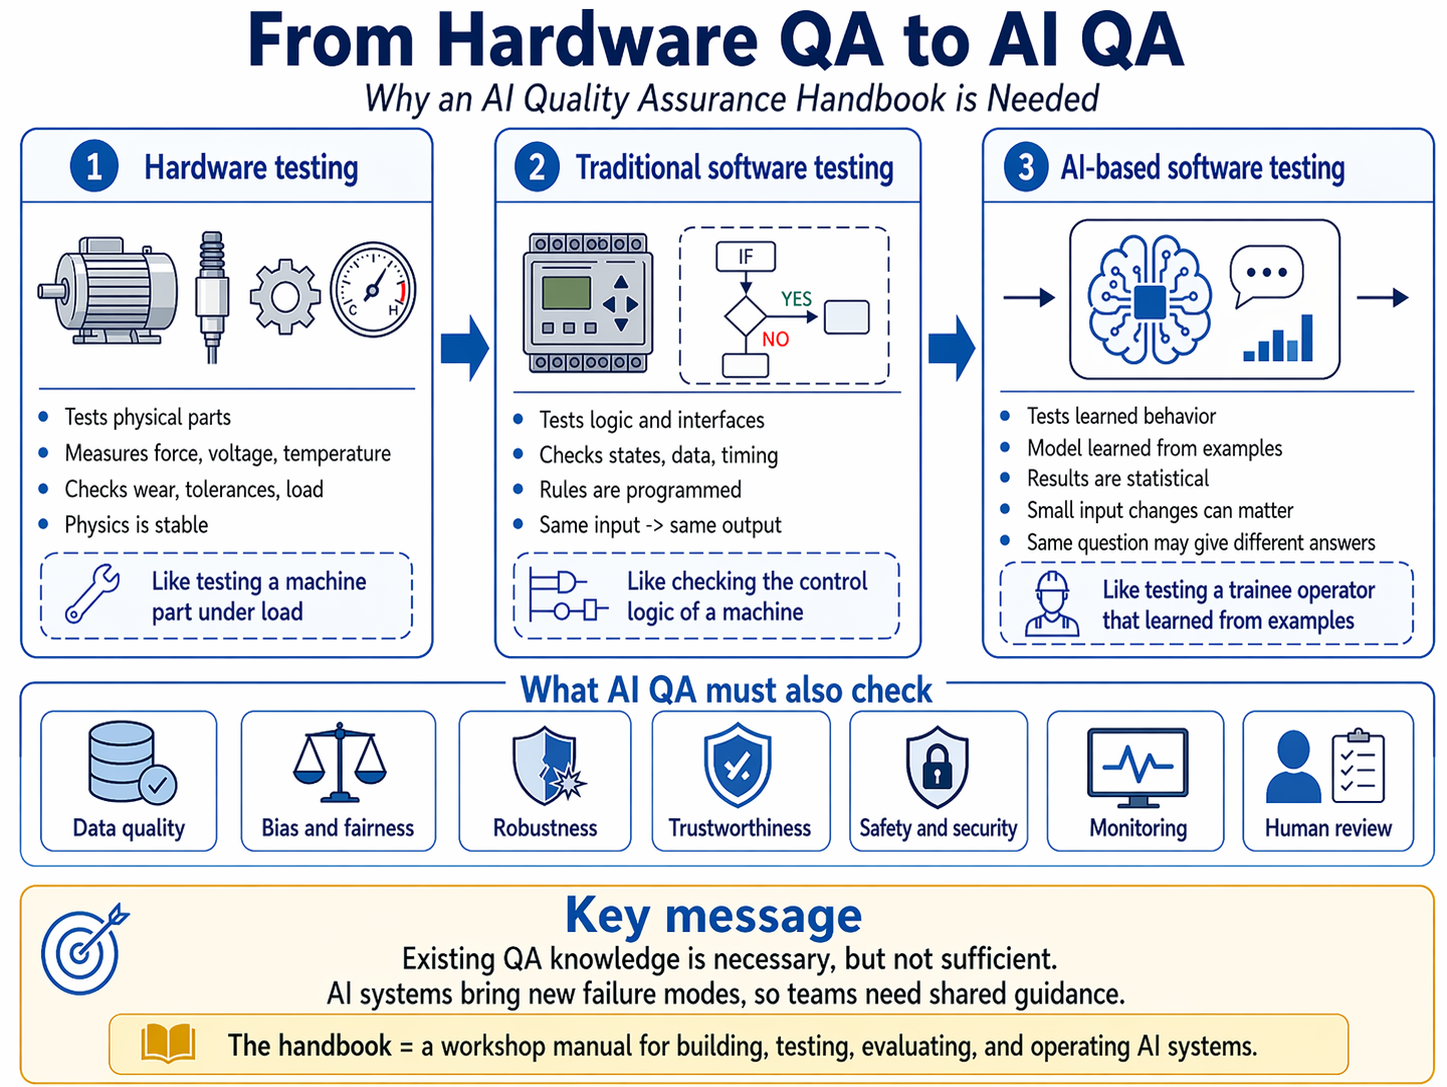
\includegraphics[keepaspectratio]{img/HW-SW-AI-test-differencesV2.png}}

}

\caption{Cover of the ``AI QA Workbook''}

\end{figure}%

For a mechatronic engineer, testing often starts with something
physical: a sensor, a motor, a controller, a brake, a robot arm. You can
measure force, voltage, temperature, speed, wear, or vibration. The
system may be complex, but the laws of physics are stable. Software
testing is different.

Testing of Software, because it has no material fatigue, but it has
logic, states, interfaces, data, timing, and dependencies. A small
change in one line of code can change the whole system behavior. Testing
software is therefore less like testing a gear under load, and more like
checking the control logic of a whole machine in many operating
situations.

Testing AI-based software is another step further. Traditional software
is like a machine built from drawings. The developer defines the rules.
The tester checks whether the system follows these rules. AI-based
software is more like a machine that has learned from examples. The
rules are not always explicitly programmed. They are hidden inside a
model. This creates new QA challenges: the system may be statistically
correct, but still wrong in important edge cases. It may behave
differently with slightly different input data. For generative AI and
chatbots, the same question can even lead to different answers.

A simple metaphor:

\begin{itemize}
\tightlist
\item
  Hardware testing checks whether the machine part can carry the load.
\item
  Traditional software testing checks whether the control logic follows
  the specification.•
\item
  AI testing checks whether a learned behavior is reliable, safe, fair,
  robust, and useful under real-world conditions.
\end{itemize}

This is why AI quality assurance needs more than normal test cases. It
needs test data, evaluation datasets, statistical metrics, bias checks,
robustness checks, monitoring, and human judgement. The ISTQB AI Testing
syllabus highlights that AI systems need attention to AI-specific
quality characteristics, acceptance criteria, data quality, test
oracles, statistical testing, and risk-based testing. ISO/IEC TR
29119-11 also emphasizes typical AI challenges such as bias,
non-determinism, complexity, explainability, and the test oracle
problem.

The planned interactive workbook should help testers and developers
learn these differences step by step. It should be a practical workshop
manual, not a theory book. Like a maintenance manual for a complex
machine, it should explain what to inspect, which risks to expect, which
measurements to take, and which warning signs matter.

The key message for creating this work is simple:

\begin{tcolorbox}[enhanced jigsaw, arc=.35mm, bottomrule=.15mm, bottomtitle=1mm, breakable, colback=white, colbacktitle=quarto-callout-tip-color!10!white, colframe=quarto-callout-tip-color-frame, coltitle=black, left=2mm, leftrule=.75mm, opacityback=0, opacitybacktitle=0.6, rightrule=.15mm, title=\textcolor{quarto-callout-tip-color}{\faLightbulb}\hspace{0.5em}{Tip \ref*{tip-why-workbook}: Why a AI-QA Workbook?}, titlerule=0mm, toprule=.15mm, toptitle=1mm]

\quartocallouttip{tip-why-workbook} 

\begin{itemize}
\tightlist
\item
  AI systems introduce new failure modes.
\item
  Existing QA knowledge is necessary, but not sufficient.
\item
  The workbook will help the organization build a shared, practical
  competence base for testing and evaluating AI-based systems safely and
  efficiently.
\end{itemize}

\end{tcolorbox}

\section*{How to read this workbook?}\label{how-to-read-this-workbook}
\addcontentsline{toc}{section}{How to read this workbook?}

\markright{How to read this workbook?}

Select your own reading path!

\includegraphics[width=6.94in,height=1.81in]{index_files/figure-latex/mermaid-figure-1.png}

\includegraphics[width=6.78in,height=0.73in]{index_files/figure-latex/mermaid-figure-2.png}

This is a Quarto book. To learn more about Quarto books visit
\url{https://quarto.org/docs/books}.

\bookmarksetup{startatroot}

\chapter{Introduction}\label{introduction}

This is a book created from markdown and executable code.

See Knuth (1984) for additional discussion of literate programming.
Another reference is De Angelis et al. (2023),

\part{Start Here - AI QA Basics}

\chapter{Introduction to Artificial
Intelligence}\label{introduction-to-artificial-intelligence}

\section{Introduction to AI}\label{introduction-to-ai}

Adapted from
\href{https://istqb.org/certifications/certified-tester-ai-testing-ct-ai/}{ISTQB
Certified Tester - AI Testing Syllabus}; other sources are cited in the
text.

This chapter introduces key distinctions between conventional and
AI-based system{}s, focusing on their design approaches, adaptability,
and explainability. It describes the spectrum of AI capabilities,
ranging from narrow AI to general AI and super AI, and outlines core
technologies such as ML, deep learning, and GenAI. The chapter describes
common hardware and development environments for AI-based systems, as
well as popular ML frameworks. Finally, it considers essential
regulatory and technical standards that guide responsible AI development
and deployment within various domains.

\subsection{AI-Based and Conventional
Systems}\label{ai-based-and-conventional-systems}

Conventional computer systems are typically programmed using imperative
languages, where human developers explicitly define step-by-step
instructions, including constructs such as if-then-else statements and
loops. This deterministic approach helps make the system's behavior
predictable and transparent, making it easier for humans to understand
how inputs produce different outputs. In contrast, most AI{}-based
systems, particularly those leveraging ML{}, do not follow predefined
rules. Instead, they analyze patterns in the data to determine how to
respond to new inputs. For example, an AI-based image recognition system
trained to identify cats does not rely on explicitly coded rules.
Instead, it learns from a dataset of cat images, extracting patterns
that it later applies to unseen images to classify them accurately.

One fundamental difference between conventional and AI-based systems{}
is how they approach problem-solving. Many AI-based systems rely on
probabilistic reasoning, statistical inference, and pattern recognition
to generate results. This allows AI models to handle complex forms of
uncertainty and ambiguity more effectively, resulting in outputs that
are not always predictable.

A key challenge in AI-based systems is explainability. Many AI models,
particularly deep learning architectures, can contain billions of
parameters, making their internal workings difficult for humans to
interpret. This ``black-box'' nature raises concerns in critical domains
such as healthcare, finance, defence, and transportation, where
understanding why an AI model made a particular decision is crucial.
Achieving transparency (see 2.1.1) and explainability in AI-driven
decision-making has become a critical focus in AI regulation.

Another significant distinction is adaptability. Conventional systems
are static and typically require manual updates to incorporate new
knowledge or respond to environmental changes. AI-based systems, in
contrast, can be self-learning, continuously improving their performance
as they encounter new data. This adaptability makes AI particularly
powerful in dynamic environments. Adaptability also requires continuous
monitoring to maintain ongoing alignment with core requirements.

\subsection{Narrow AI, General AI, and Super
AI}\label{narrow-ai-general-ai-and-super-ai}

Narrow AI{}, also known as weak AI, is designed to perform specific
tasks and represents all deployed AI systems in use today. Narrow
AI-based systems operate within a limited domain and can be highly
efficient at solving specialized problems, such as image recognition,
speech processing, and language translation. However, they lack the
ability to generalize beyond the functions they have learned. For
instance, an AI-based system that excels at recognizing faces cannot
perform language translation unless it is explicitly retrained to do so.
Frontier AI{}, a subset of narrow AI, represents the most advanced form
of these systems, pushing the boundaries of current capabilities with
GenAI models. Frontier AI includes large-scale systems with highly
autonomous decision-making capabilities; however, they remain
task-specific and have not yet achieved the versatility of general AI.

General AI{}, also known as strong AI, refers to an AI-based system that
possesses the ability to perform most intellectual tasks that a human
can. General AI would be able to understand, learn, and apply knowledge
across a broad range of tasks without needing to be retrained for each
new task. This type of AI would exhibit human-like reasoning and
adaptability, capable of solving unfamiliar problems in various domains,
much like humans do. Despite significant progress in AI, no AI-based
system today possesses general intelligence.

Super AI{} (artificial superintelligence) is the form of AI in which an
AI-based system continuously improves itself without~the need for human
intervention or control. For Super AI to be possible, access to the
Internet is not strictly required, but such access could significantly
expand its capabilities and influence. It would surpass human
intelligence and general AI, which many believe would pose an
existential risk to humanity. The point at which AI-based systems
transition from general AI to super AI, if it were to occur, is commonly
known as the technological singularity.

\subsection{Different Types of AI
Technologies}\label{different-types-of-ai-technologies}

Artificial Intelligence encompasses a range of technologies, each suited
to specific tasks and challenges. One of the core branches of AI is
ML{}, which enables systems to learn from data and build models without
explicit programming. While some MLS can adapt and improve continuously
with new data throughout their lifetimes, others operate on the
knowledge they initially learned and require explicit retraining to
update their capabilities. ML includes several approaches:

\begin{itemize}
\item
  Supervised learning{} utilizes labeled data and algorithms, such as
  linear regression and decision trees, for tasks like prediction and
  classification.
\item
  Unsupervised learning{} uncovers patterns in unlabeled data through
  techniques like clustering (using clustering algorithms).
\item
  Reinforcement learning{} enables intelligent agents to learn optimal
  behaviors through trial-and-error interactions with their environment.
\end{itemize}

Key ML technologies include neural networks, Bayesian models, support
vector machines (SVM) and random forests. See Chapter 3 for more on ML.

Deep Learning (DL), a subset of ML methods, uses deep neural networks to
solve complex problems. For example:

\begin{itemize}
\item
  Convolutional neural networks (CNN) are highly effective for image
  recognition and object detection.
\item
  Recurrent neural networks (RNN) specialize in processing sequential
  data, such as text or time series.
\item
  Transformers handle long-range dependencies in sequences, powering
  models for natural language processing and vision transformers for
  images.
\end{itemize}

GenAI builds on these technologies to create new content, including
text, images, and audio (see 1.1.4). This is driven by models such as
LLM, which combine deep neural networks (DNN) with natural language
processing (NLP) to analyze and generate human-like language.

Other specialized AI technologies include:

\begin{itemize}
\item
  NLP for language analysis, including tasks like sentiment analysis and
  machine translation.
\item
  Computer vision for analyzing visual data, supporting applications
  like facial recognition and robotics.
\item
  Fuzzy logic for reasoning under uncertainty.
\item
  Search algorithms for solving optimization problems, such as
  navigation, and strategic decision-making.
\item
  Rule-based reasoning systems, or expert systems, for structured
  decision support.
\end{itemize}

Although the full integration of these AI technologies remains limited,
new developments such as LLM demonstrate the potential to combine
different AI technologies into unified, intelligent systems. Agentic AI
extends these technologies through autonomous agents that plan, reason,
and act independently to achieve goals in dynamic environments.

\section{Generative AI}\label{generative-ai}

Generative AI (GenAI){} refers to AI-based systems specialized in
creating new content, such as text, images, video, music, or complex
data, while many also support classification and prediction. These
systems learn from vast amounts of data to produce outputs that resemble
their training data, enabling a wide range of creative and practical
applications.

The main technologies behind GenAI include generative adversarial
networks (GANs), diffusion models, and transformers. GANs use two neural
networks in competition to create highly realistic synthetic data.
Diffusion models generate content by gradually adding and then removing
noise from data, resulting in high-quality outputs. Transformer models,
which underpin LLM, utilize self-attention mechanisms to generate
coherent and contextually relevant text, and are increasingly being
adapted for multimodal tasks.

Beyond their technical foundations, GenAI systems raise significant
societal and ethical concerns. Misuse is a major concern: these models
can be exploited to create deepfakes, spread misinformation, or generate
convincing fraudulent content, thereby undermining trust in digital
media and public discourse. The ease of producing synthetic content
amplifies risks related to privacy, security, and manipulation, but it
can bring notable benefits and opens opportunities for innovation in
entertainment, marketing, education, and research.

The impact on employment is also notable, particularly among
white-collar professions. As GenAI automates tasks such as writing,
design, coding, and even legal or medical documentation, there is
increasing debate about potential job displacement. While these
technologies can boost productivity and foster new creative
opportunities, they may also lead to workforce disruption and
necessitate widespread reskilling.

Sustainability is another pressing issue. Training and running large
GenAI models involve substantial computational resources, resulting in
high energy consumption and a significant carbon footprint. This
environmental impact has prompted calls for more efficient model designs
and greener infrastructure.

Most practical GenAI tools today are based on foundation models, which
are then fine-tuned for specific applications. The field is also
advancing toward multimodal models capable of processing and generating
content across text, images, and audio, enabling richer, more flexible
AI-based systems. Regulatory frameworks, such as the EU AI Act {[}EU AI
Act{]}, are emerging to guide the responsible development and use of
these technologies.

For more on GenAI and testing, see
\href{https://istqb.org/certifications/gen-ai/}{Certified Tester --
Testing with Generative AI (CT-GenAI)}.

\section{Machine Learning Development
Frameworks}\label{machine-learning-development-frameworks}

ML development framework{}s provide a toolkit for building and training
ML models. Typical functionality provided by these frameworks includes:

\begin{itemize}
\item
  \textbf{Data Handling:} They assist with loading, preprocessing, and
  managing the data used to train and test the model. This might involve
  cleaning, formatting, and transforming the data into a suitable format
  for the chosen model.
\item
  \textbf{Model Building:} These frameworks offer libraries of ML
  algorithms and tools to design the architecture of the constructed ML
  model. This includes specifying the type of model (e.g., neural
  network, decision tree), the number of layers and connections, and the
  mathematical operations performed within the model.
\item
  \textbf{Training and Optimization:} Frameworks provide algorithms that
  iteratively adjust the model's internal parameters based on the
  training data and on the desired result. The goal is to optimize the
  model's performance in accomplishing the desired task (e.g.,
  classification, ML regression). Some frameworks may support
  distributed training and enhance or fine-tune pretrained models.
\item
  \textbf{Evaluation:} They offer tools to evaluate how well the trained
  model performs on unseen data. This might involve measuring accuracy,
  precision, and recall for classification tasks, or error rates for ML
  regression tasks (see 3.1.1).
\item
  \textbf{Deployment:} Some frameworks provide capabilities for
  deploying the trained model for real-world use. This could involve
  converting the model into a format suitable for integration with web
  applications, mobile devices, edge devices or embedded systems.
\end{itemize}

These frameworks can operate at different levels of abstraction. Some
offer a lower-level application programming interface (API), providing
developers with more control over model building but requiring more
coding expertise. Others offer a higher-level API, simplifying model
creation but offering fewer customization options.

Different frameworks can focus on different application domains. Some
are general purpose and support a wide range of application areas. In
contrast, others are more specialized, focusing on specific areas such
as image recognition, speech recognition, and language translation.

Selecting the most appropriate framework can depend on several factors,
such as:

\begin{itemize}
\item
  the application area;
\item
  the need for a user-friendly interface for rapid prototyping;
\item
  configurability for complex models;
\item
  the expertise of the users;
\item
  deployment considerations, as some frameworks are better suited for
  resource-constrained environments;
\item
  level of (community) support;
\item
  ecosystem maturity.
\end{itemize}

\textbf{TBD} add more on popular frameworks such as TensorFlow, PyTorch,
Keras, Scikit-learn, Hugging Face Transformers, and others.

\chapter{}\label{section}

\chapter{AI Quality Characteristics and
Risks}\label{ai-quality-characteristics-and-risks}

\section{ISO 25000-Series Software Quality
Standards}\label{iso-25000-series-software-quality-standards}

The ISO 25000 series of standards defines software quality
characteristics and sub-characteristics. These characteristics can be
used to evaluate the quality of software, including AI systems. The main
characteristics include:

\begin{itemize}
\item
  \textbf{Functional suitability}: The degree to which the software
  meets the specified requirements and performs its intended functions.
\item
  \textbf{Performance efficiency}: The degree to which the software
  performs its functions efficiently, including response time, resource
  utilization, and throughput.
\item
  \textbf{Compatibility}: The degree to which the software can operate
  with other software, hardware, or systems.
\item
  \textbf{Usability}: The degree to which the software can be used by
  specified users to achieve specified goals with effectiveness,
  efficiency, and satisfaction.
\item
  \textbf{Reliability}: The degree to which the software can maintain
  its performance under specified conditions for a specified period of
  time.
\item
  \textbf{Security}: The degree to which the software protects
  information and data from unauthorized access, use, disclosure,
  disruption, modification, or destruction.
\item
  \textbf{Maintainability}: The degree to which the software can be
  modified to correct faults, improve performance, or adapt to a changed
  environment.
\end{itemize}

\subsection{ISO 25059:2023 - Quality Model for AI-Based
Systems}\label{iso-250592023---quality-model-for-ai-based-systems}

The ISO/IEC 25059:2023 standard extends the ISO 25000 series to
specifically address the quality characteristics of AI-based systems. It
introduces new and partially adapt existing characteristics and
sub-characteristics that are relevant to AI, such as AI functional
correctness, functional adaptability, user controllability,
transparency, AI robustness, and intervenability. Additionally, it
emphasizes the importance of societal and ethical risk mitigation in the
context of AI systems. Major AI safety challenges, such as vague
specifications, non-determinism, self-learning, limited explainability,
and evolving standards, are also addressed, with an emphasis on their
impact on testing and regulation. This standard provides a framework for
evaluating the quality of AI-based systems and can guide the development
and testing processes to ensure that these systems meet the necessary
quality standards.

\subsection{AI-Specific Quality
Characteristics}\label{ai-specific-quality-characteristics}

The ISO/IEC 25059 proposes to evaluate AI-based systems from two
perspectives: product quality and quality in use. From a testing
perspective, these quality characteristics directly influence how test
objectives are defined, how acceptance criteria are formulated, and how
test results are interpreted for AI-based systems.

New and modified characteristics, compared to ISO/IEC 25010, include:

\begin{itemize}
\item
  AI functional correctness{} (product quality): AI-based systems,
  especially those using probabilistic ML, cannot guarantee perfect
  accuracy. Since a certain error rate is expected in AI outputs, the
  concept of functional correctness has been adjusted accordingly.
  ISO/IEC 25059 evaluates functional correctness by considering both
  correct and incorrect outputs and by defining acceptable thresholds
  for incorrect results, reflecting the inherent variability in AI-based
  system outputs (see Section~\ref{sec-metrics-for-classification}).
\item
  Functional adaptability{} (product quality): a new sub-characteristic
  of functional suitability. The ability of the AI-based system to
  autonomously adapt to changes in its operational environment after it
  is deployed.
\item
  User controllability{} (product quality): a new sub-characteristic of
  interaction capability (note that interaction capability is itself a
  new term that replaces usability in the 2023 version of ISO/IEC
  25010). A property of an AI-based system such that a human or another
  external agent can intervene in its functioning in a timely manner.
\item
  Transparency{} (product quality and quality in use): a new
  sub-characteristic of interaction capability and a new
  sub-characteristic of satisfaction. It relates to the degree to which
  appropriate information about the AI-based system is communicated to
  stakeholders (see 6.1.2).
\item
  AI robustness{} (product quality): a new sub-characteristic of
  reliability. It describes the ability of an AI-based system to
  maintain its level of AI functional correctness regardless of
  circumstances, such as the presence of biased, adversarial, or invalid
  data inputs, external interference, adverse environmental conditions,
  and operator misuse.
\item
  Intervenability{} (product quality): a new sub-characteristic of
  security. The degree to which an operator can intervene in an AI-based
  system's functioning in a timely manner to prevent harm or hazard.
\item
  Societal and ethical risk mitigation{} (quality in use): a new
  sub-characteristic of `Freedom from risk'. Considers many areas to
  mitigate societal and ethical risk, including accountability, fairness
  and non-discrimination, professional responsibility, promotion of
  human values, privacy, safety and security, human control of
  technology, community involvement and development, human-centered
  design, respect for the rule of law, respect for international norms
  of behavior, environmental sustainability, and labor practices.
\end{itemize}

\subsection{\texorpdfstring{AI and
Safety{}}{AI and Safety}}\label{ai-and-safety}

Safety-related systems have the potential to cause injury or harm to
people, property or the environment. Developing and testing non-AI
safety-related systems can take a lot of effort, but is feasible;
however, for AI-based systems, there are several additional challenges:

\begin{itemize}
\item
  Specifications: In traditional safety-related systems, requirements
  are defined for the complete system and refined until the developer
  can transform them into code. The requirements for many AI-based
  systems often begin with vague goals and are then implicitly provided
  via the training data that encodes patterns, rules, and objectives,
  without fully formalizing every detail upfront. This can mean that the
  necessary traceability from requirements to implementation is
  inadequate for AI-based systems.
\item
  Non-determinism{}: This characteristic of many AI-based systems makes
  it inherently challenging to guarantee the precise behavior of these
  systems. Even rigorously tested models can exhibit unexpected behavior
  due to factors such as random number generation or slight variations
  in input values.
\item
  Self-learning{}: Rigorous testing is used to demonstrate the safety
  integrity of a system before deployment. For self-learning AI-based
  systems, this is undermined as the system's behavior progressively
  moves away from the originally tested behavior. Managing how the model
  learns and the data it uses can sometimes help to avoid the emergence
  of new problematic behaviors. Alternatively, safety guards can be
  implemented to help prevent the model from learning or making
  decisions that could compromise safety (e.g., a content moderation
  component to filter prompts).
\item
  Explainability{} and Transparency{}: For safety-related systems, it is
  essential to understand how and why the system makes decisions.
  However, the decision-making processes of AI-based systems are often
  not transparent. Explainable AI techniques, such as LIME (Local
  interpretable model-agnostic explanations), can provide insights into
  the AI-based system's reasoning; however, they are not widely
  available and may compromise system performance.
\item
  Evolving Regulations: The regulatory landscape for safety-related
  AI-based systems is constantly evolving. The use of AI is currently
  not included in mature functional safety international standards, and
  some of these standards even prohibit its use in such systems. The EU
  AI Act {[}EU AI Act{]} (see 1.1.8) classifies AI systems used as
  safety components (such as in aviation, medical devices, or
  automotive) as high-risk and imposes strict requirements on their
  development and testing.
\end{itemize}

\section{Acceptance Criteria for AI-Based
Systems}\label{acceptance-criteria-for-ai-based-systems}

This section outlines acceptance criteria related to the quality
characteristics specified in the ISO/IEC 25059 standard, as well as
safety. For AI-based systems, acceptance criteria often need to be
statistical, probabilistic, or threshold-based rather than binary, which
introduces additional testing challenges.

\subsection{Acceptance Criteria for AI-Based
Systems}\label{acceptance-criteria-for-ai-based-systems-1}

When evaluating the quality of an AI-based system, it is essential to
consider both functional and non-functional quality characteristics.
This helps confirm that the AI-based system functions as intended and
satisfies broader quality requirements. The ISO/IEC 25010 and ISO/IEC
25059 standards provide a comprehensive framework for defining software
quality. In this section, the focus is on the acceptance criteria
associated with the quality characteristics specific to AI (i.e., those
defined in ISO/IEC 25059) and safety (see 2.1.2).

The following table lists example acceptance criteria for safety and
each of the quality characteristics defined in the ISO/IEC 25059
standard.

Characteristic

Example Acceptance Criteria

AI functional correctness{} (see
Section~\ref{sec-metrics-for-classification})

Accuracy of 95\% for an image recognition system.

Recall of 90\% for a defect prediction system.

Functional adaptability{}

A maximum of 20 seconds for the engine management system to adapt when
it crosses a specified altitude threshold.

A video streaming service shall adjust its homepage to recommend at
least 40\% of documentaries after a user watches three full-length
documentaries in a single session.

User controllability{}

A supervisor can take control of an autonomous drone within 0.5 of a
second when it sends a distress signal due to loss of its GPS location.

The farm control system notifies the farmer when the sensor's visual
performance degrades by more than 30\%, allowing immediate manual
override; it fully deactivates if degradation exceeds 50\% without user
response.

Transparency{}

Sufficient information is provided about the third-party ML model and
the provenance of its training data to meet the requirements of the
relevant company standard.

The system's operational dashboard and API must provide an endpoint that
returns the unique version identifier of the currently deployed
prediction model and a link to its corresponding documentation.

AI robustness{}

The response time for the AI-based security penetration alert system
predictions remains below 1 second when access to the central
vulnerabilities database is disrupted for 30 seconds.

The edge AI device shall automatically transition to a lower-fidelity,
reduced-power inference mode (instead of crashing) when its internal
operating temperature exceeds 85°C for a continuous period of 10
seconds.

Intervenability{}

If a robot breaches its safety zone, the production line is capable of
being shut down within 0.5 seconds after a shutdown is initiated.

To prevent potential blackouts, the power grid management system shall
provide a 30-second confirmation window, during which an engineer can
veto any AI-proposed action classified as `critical' before it is
automatically executed.

Societal and ethical risk mitigation{}

The automated prison sentencing system does not discriminate between
racial groups based on the specified fairness metric.

The chatbot must pass an internal ``red teaming'' assessment with a
score of 95\% or higher, demonstrating its refusal to generate content
that promotes violence, self-harm, or hate speech.

Safety{}

Non-AI components of the AI-based steering control system are compliant
with ISO 26262-6 at ASIL (automotive safety integrity level) C.

100\% of the relationships between inputs and outputs of the ML model in
the nuclear power plant control system can be mapped with an average
accuracy of no lower than 99.9\% by an explainability tool.

Control signals that exceed specified safety limits by more than 10\%
are analyzed and regulated within 0.15 seconds after being detected by
the safety monitoring sub-system.

\chapter{Detailed Preview on ISO/IEC DIS
25059:2026}\label{detailed-preview-on-isoiec-dis-250592026}

This document was prepared by Joint Technical Committee ISO/IEC JTC~1,
\emph{Information technology}, Subcommittee SC~42, \emph{Artificial
intelligence}.

This second edition cancels and replaces the first edition
(\href{https://www.iso.org/obp/ui/\#iso:std:iso-iec:25059:ed-1:v1:en}{ISO/IEC
25059 :2023}), which has been technically revised.

The main changes are as follows:

\begin{itemize}
\item
  --- alignment with the revised version of
  \href{https://www.iso.org/obp/ui/\#iso:std:iso-iec:25010:ed-2:v1:en}{ISO/IEC~25010:2023};
\item
  --- alignment with the revised version of
  \href{https://www.iso.org/obp/ui/\#iso:std:iso-iec:25019:ed-1:v1:en}{ISO/IEC~25019:2023};
\item
  --- addition of an \textbf{AI service quality model} based on
  \href{https://www.iso.org/obp/ui/\#iso:std:iso-iec:ts:25011:ed-1:v2:en}{ISO/IEC
  TS 25011:2017};
\item
  --- addition of \textbf{``Environmental sustainability''} as a
  sub-characteristic of ``Performance efficiency'' in the product
  quality model.
\end{itemize}

\textbf{2~~~Normative references}

The following documents are referred to in the text in such a way that
some or all of their content constitutes requirements of this document.
For dated references, only the edition cited applies. For undated
references, the latest edition of the referenced document (including any
amendments) applies.

\begin{itemize}
\item
  \href{https://www.iso.org/obp/ui/\#iso:std:iso-iec:25010:ed-2:v1:en}{ISO/IEC~25010:2023}
  Systems and software engineering --- Systems and software Quality
  Requirements and Evaluation (SQuaRE) --- Product quality model
\item
  \href{https://www.iso.org/obp/ui/\#iso:std:iso-iec:25019:ed-1:v1:en}{ISO/IEC~25019:2023}
  Systems and software engineering --- Systems and software Quality
  Requirements and Evaluation (SQuaRE) --- Quality-in-use model
\item
  \href{https://www.iso.org/obp/ui/\#iso:std:iso-iec:22989:ed-1:v1:en}{ISO/IEC~22989:2022}
  Information technology --- Artificial intelligence --- Artificial
  intelligence concepts and terminology
\item
  \href{https://www.iso.org/obp/ui/\#iso:std:iso-iec:23053:ed-1:v1:en}{ISO/IEC~23053:2022}
  Framework for Artificial Intelligence (AI) Systems Using Machine
  Learning (ML)
\end{itemize}

\section{5 Product quality model}\label{product-quality-model}

An AI system product quality model is detailed in Table 1. The model is
based on a modified version of a general system model provided in
ISO/IEC 25010. New and modified sub-characteristics are identified using
a lettered footnote. Some of the sub-characteristics have different
meanings or contexts as compared to the ISO/IEC 25010 model. The
modifications, additions and differences are described in this clause.

The unmodified original characteristics are part of the AI system
product model and shall be interpreted in accordance with ISO/IEC 25010.
Each of these modified or added sub-characteristics are listed in the
remainder of this clause.

Table 1 --- AI system product quality model

Functional suitability

Security

Functional completeness

Confidentiality

Functional correctness m

Integrity

Functional appropriateness

Non-repudiation

Functional adaptability a

Accountability

Performance efficiency

Authenticity

Time behaviour

Resistance

Resource utilization

Intervenability a

Capacity

Maintainability

Environmental sustainability a

Modularity

Interaction capability

Reusability

Appropriateness recognisability

Analysability

Learnability

Modifiability

Operability

Flexibility

User error protection

Testability

User engagement

Adaptability

Inclusivity

Scalability

User assistance

Installability

Self descriptiveness

Replaceability

User controllability a

Safety

Transparency a

Operational constraint

Reliability

Risk identification

Faultlessness

Fail safe

Availability

Hazard warning

Fault tolerance

Safe integration

Recoverability

Compatibility

Robustness a

Co-existence

Interoperability

NOTE

\hl{a Added sub-characteristics}.

\hl{m Modified sub-characteristics.}

\textbf{3.2 Product quality}

\textbf{3.2.1 user controllability}

degree to which a user can appropriately intervene in an AI system's
functioning in a timely manner

\textbf{3.2.2 functional adaptability}

degree to which an AI system can accurately acquire information from
data, or the result of previous actions, and use that information in
future predictions

\textbf{3.2.3 functional correctness}

degree to which a product or system provides the correct results with
the needed degree of precision Note 1 to entry: AI systems, and
particularly those using machine learning models, do not usually provide
functional correctness in all observed circumstances.

{[}SOURCE: ISO/IEC 25010:2023, 4.2.1.2, modified --- Note to entry
replaced.{]}

\textbf{3.2.4 intervenability}

degree to which an operator can intervene in an AI system's functioning
in a timely manner to prevent harm or hazard

\textbf{3.2.5 robustness}

degree to which an AI system can maintain its level of functional
correctness under any circumstances

\textbf{3.2.6 environmental sustainability}

state in which the ecosystem and its functions are maintained for the
present and future generations

{[}SOURCE: ISO 17889-1:2021, 3.1.1, modified --- generation made
plural.{]}

\textbf{Added / Modified Subcharacteristics}

\textbf{\hl{5.4 Functional correctness}}

Functional correctness exists in ISO/IEC 25010. The AI system product
quality model amends the description since AI systems, and particularly
probabilistic ML methods, do not usually provide functional correctness
because a certain error rate is expected in their outputs. Therefore, it
is necessary to measure correctness and incorrectness carefully.
Numerous measurements exist for these purposes in the context of ML
methods and examples of these as applicable to a classification model
can be found in ISO/IEC 4213.

Additionally, there can be a trade-off between characteristics such as
performance efficiency{[}37{]}, robustness{[}38{]} and functional
correctness.

Annex C provides further information about why functional correctness is
preferred to other terms such as the more general performance to
describe the correctness of the model.

\textbf{\hl{5.3 Functional adaptability}}

Functional adaptability is a new sub-characteristic of functional
suitability. Functional adaptability of an

AI system is the ability of the system to adapt itself to a changing
dynamic environment it is deployed in.

AI systems can learn from new training data, production data and the
results of previous actions taken

by the system. The concept of functional adaptability subsumes that of
continuous learning, as defined in ISO/IEC 22989:2022, 5.11.9.2.

Continuous learning is not a mandatory requirement for functional
adaptability. For example, a system

that switches classification models based on events in its environment
can also be considered functionally adaptive.

Functional adaptability in AI systems is unlike other quality
characteristics as there are system specific consequences that cannot be
interpreted using a straight-line linear scale (e.g.~bad to good).
Generally, higher functional adaptability can result in improvements for
the outcomes enacted by AI systems.

For some systems, high functional adaptability can cause additional
unhelpful outcomes to become more likely based on the system's previous
choices. Weightings of a decision path with relatively high uncertainty,
reinforced based on previous AI system decisions, can result in higher
likelihood of unintended negative outcomes. In this fashion, functional
adaptability can reinforce negative human cognitive biases.

While conventional algorithms usually produce the same result for the
same set of inputs, AI systems, due to continuous learning, can exhibit
different behaviour and therefore can produce different results.

\textbf{\hl{5.8 Environmental sustainability}}

The sustainability domain requires organization to consider three main
areas, each with their own sustainability aspects:

--- economic sustainability;

--- social sustainability;

--- environmental sustainability.

To date, the focus of AI practitioners has been mostly on environmental
and social sustainability. Social sustainability is addressed in AI
trustworthiness standards ISO 26000, ISO/IEC TR 24368, ISO/IEC TS 12791
and ISO/IEC 12792.

The environmental sustainability of AI systems affects many ecosystems
in a complex manner. Organizations are only at the beginning of fully
understanding and addressing these environmental sustainability aspects.

The environmental sustainability of AI is an emerging discipline.
However, practitioners can find guidance with regards to the
environmental sustainability of AI applications, AI ecosystems and the
AI system lifecycle, as well as metrics to measure and manage certain
aspects thereof, in the following standards:

--- environmental sustainability aspects of AI systems, including
ISO/IEC TR 20226;

--- the life cycle assessment of an AI system, including ISO 14040, EC
JRC life cycle assessment;

--- methods for measuring resource usage, including software
carbon-intensity, water usage, and energy usage, including ISO/IEC
21031;

--- environmental management, including ISO 14001;

--- methods for measuring and assessing the environmental impact of an
AI system (including greenhouse gas emissions), including ISO 14064-1,
ISO/IEC 21031, IEEE 1922.2, ITU-T L.1480;

--- methods for a circular economy, including ISO 59020.

Depending on the stakeholder role of the user applying these standards,
as well as the phase of the AI system lifecycle in which the standard is
applied, what they measure will vary on a case-by-case basis. For
example, a designer for an AI application can include requirements for
software carbon intensity (SCI) as discovered through ISO/IEC TR 20226,
a developer may implement it using ISO/IEC 21031, and an organization
using the AI application can use the output of the metric in its
greenhouse gas emission reporting.

ISO/IEC TR 20226 describes environmental sustainability aspects of AI
systems.

\textbf{\hl{5.6 Transparency}}

Transparency is sub-characteristic of interaction capability in the
product quality model and a subcharacteristic of satisfaction in the
quality in use model. It relates to the degree to which appropriate
information about the AI system is communicated to stakeholders (see
ISO/IEC 22989:2022, 5.15.8).

Transparency of AI systems can help potential users of AI systems to
choose a system to fit their requirements, improving stakeholders'
knowledge about the applicability and the limitations of an AI system,
and assisting with the explainability of AI systems.

The transparency information can include a description of an AI system
functionality, the system's decomposition, interfaces, ML models used,
training data, verification and validation data, performance benchmarks,
logs and the management practices of an organization responsible for the
system.

Transparent AI systems document, log or display their internal processes
using introspection tools and data files. The flow of data can be
trackable at each step, with applied decisions, exceptions and rules
documented. Log output can track processes in the pipeline as they
permute data, as well as system level calls. Errors are logged
explicitly, particularly in transform steps. Highly transparent AI
systems can be built of well-documented subcomponents whose interfaces
are explicitly described. The transparency of AI systems eases
investigations of system malfunctions.

A system with low transparency has internal workings which are difficult
to inspect externally. Unavailability of detailed processing records can
impair testability and societal and ethical impact assessment and risk
treatment.

Ultimately, transparency of AI systems contributes to establishing of
trust, accountability and communication among stakeholders. Some aspects
of transparency are discussed in ISO/IEC 12792 and ISO/IEC TS 6254.

\textbf{\hl{5.5 Robustness}}

Robustness is a new sub-characteristic of reliability. It is used to
describe the ability of a system to maintain its level of functional
correctness (see Annex C for discussion on the term performance) under
any circumstances including:

--- the presence of unseen, biased, adversarial or invalid data inputs;

--- external interference;

--- environmental conditions encompassing generalization, resilience,
reliability;

--- attributes related to the proper operation of the system as intended
by its developers.

The proper operation of a system is important for the security of the
system and safety of its stakeholders in a given environment or context.
Information about functional safety in the context of AI systems can be
found in the ISO/IEC TS 22440 series (ISO/IEC TS 22440-1, ISO/IEC TS
22440-2 and ISO/IEC TS 22440-3).

Robustness is discussed in ISO/IEC TR 24028:2020, 10.7 and methods for
assessment are described in ISO/IEC TR 24029-1 and defined in the
ISO/IEC 24029 series (ISO/IEC 24029-2 and ISO/IEC 24029-3).

\textbf{\hl{5.7 Intervenability}}

The extent of intervenability can be determined depending on the
scenarios where the AI system can be used. The key to intervenability is
to enable state observation and transition from an unsafe state to a
safe state. Operability is the degree to which an AI system has
attributes that enable operation and control, which emphasizes the
importance of an AI system's user interface. Compared to operability,
intervenability is more fundamental from a quality perspective and is
intended to prevent an AI system from doing harm or hazard.

Intervenability is related to controllability, which is described in
ISO/IEC TS 8200 and ISO/IEC 22989:2022, 5.15.5.

\section{Quality-in-use model}\label{quality-in-use-model}

\textbf{General}

An AI system quality-in-use model is detailed in Table 2. The model is
based on a modified version of a general quality-in-use model provided
in ISO/IEC 25019. New sub-characteristics are identified using a
lettered footnote. Some of the sub-characteristics have different
meanings or contexts as compared to the ISO/IEC 25019 model. The
additions and differences are described in this clause. The unmodified
characteristics are part of the quality-in-use model and shall be
interpreted as defined in ISO/IEC 25019.

Table 2 --- AI system quality-in-use model

Beneficialness

Risk mitigation

Usability

Economic risk mitigation

Accessibility

Environmental risk mitigation a

Suitability

Societal and ethical risk mitigation a

Acceptability

Health risk mitigation -\textgreater{} 25019

Experience

Human life risk mitigation

Trustworthiness

Compliance

Transparency a

NOTE

a Added sub-characteristics

\textbf{\hl{6.2 Transparency}}

Transparency is also a sub-characteristic of satisfaction in the product
quality model. See 5.6 for further information.

\textbf{\hl{Environmental risk mitigation}}

degree to which a product or system mitigates the potential risk to the
environment in the intended contexts of use

Note 1 to entry: environmental risk mitigation includes the mitigation
of risks that could harm the environment, such as pollution, waste, and
resource depletion. Additionally, it involves the product or system's
role in sustainability through the efficient utilization of resources,
reduction of waste, and facilitation of recycling and reuse processes.

\textbf{\hl{freedom from environmental and societal risk}}

extent to which a product (3.1.14) or system (3.1.29) mitigates the
potential risk (3.1.22) to the environment and society (3.1.23) at large
in the intended contexts of use (3.1.4)

Note 1 to entry: When a product or system is especially recognized as an
information system (3.1.9) and IT service, there is concern the
environmental and societal risk impacts on public properties in
societies, and on environments including societal or natural ecology
systems in a diverse and broad group of stakeholders (3.1.26) so that
the risk monitoring used is often considered to be more focused in
addition to risk mitigation.

\textbf{\hl{6.3 Societal and ethical risk mitigation}}

Societal and ethical risk mitigation is a new sub-characteristic of risk
mitigation. ISO/IEC TS 22443 explores this topic and outlines the
following themes:

--- accountability;

--- fairness and non-discrimination;

--- transparency and explainability;

--- professional responsibility;

--- promotion of human values;

--- privacy;

--- safety and security;

--- human control of technology;

--- community involvement and development;

--- human-centred design;

--- respect for the rule of law;

--- respect for international norms of behaviour;

--- environmental sustainability;

--- labour practices.

These themes should be considered along with the information in
\textbf{ISO/IEC TS 22443}0F{[}1{]}, with regard to the desirable
characteristics of systems in order to mitigate societal and ethical
risk.

Safety and security as well as sustainable environments are included
within the existing SQuaRE characteristics health and safety risk
mitigation, and environment risk mitigation, and therefore are not
outlined in this document.

\textbf{\hl{freedom from health risk}} extent to which a product
(3.1.14) or system (3.1.29) mitigates the potential risk (3.1.22) to
people's health in the intended contexts of use (3.1.4) (from ISO 25019:
Quality in Use Model: 3.2.2.3** )

\textbf{\hl{freedom from human life risk}}

extent to which a product (3.1.14) or system (3.1.29) mitigates the
potential risk (3.1.22) to people's lives in the intended contexts of
use (3.1.4)

\section{7 AI service quality model}\label{ai-service-quality-model}

\textbf{7.1 General}

An AI service quality model is detailed in Table 3. The model is based
on a modified version of IT service quality model provided in ISO/IEC TS
25011. New and modified sub-characteristics are identified using a
lettered footnote. Some of the sub-characteristics have different
meanings or contexts as compared to the ISO/IEC TS 25011 model. The
modifications, additions and differences are described in this clause.
The unmodified original characteristics are part of the IT service
quality model and shall be interpreted in accordance with ISO/IEC TS
25011.

Table 3 --- AI service quality model

Service quality

Service risk mitigation

Service performance

Service safety risk mitigation

Service reliability

Service security risk mitigation

Service availability

Service societal and ethical risk mitigation

Traceability a

Service adaptability a

Customizability a

\textbf{3.4.1 traceability}

degree to which the AI service outcomes can be traced to or from the
user needs

\textbf{3.4.2 service adaptability}

degree to which a service can be adapted based on factors such as
functions, responsibility, skill of

employees, communication style with users or instruments available

\textbf{3.4.3 customizability}

degree to which the AI service can be customized at the request of users

\textbf{\hl{7.2 Traceability}}

Traceability is a sub-characteristic of security. Traceability of AI
systems includes proper logging and record keeping of models, data sets,
requests and outcomes. For more information, refer to ISO/IEC 24970.

\textbf{\hl{7.3 Service adaptability}}

Service adaptability is a characteristic of the AI service quality
model. Service adaptability is influenced by digital instruments and
analysis of digital transformation. Some suggestions and improvements
can be derived from the introduction of AI systems.

Some adaptations can benefit optimizing interoperability of services,
reduction of duplications, clarifying and adapting responsibilities of
management and leadership.

Introducing measurements of efficiency and effectiveness of services can
suggest further actions of adaptability.

\textbf{\hl{7.4 Customizability}}

Customizability is a sub-characteristic of service adaptability. The
data quality and data quantity are

examples of constraints that need to be taken into consideration when
customizing an AI system.

\chapter{ISO/IEC TS 4213:2022 Information technology --- Artificial
intelligence --- Assessment of machine learning classification
performance}\label{isoiec-ts-42132022-information-technology-artificial-intelligence-assessment-of-machine-learning-classification-performance}

\href{../SomePDFs/NormenStandards/DIN_ISO_IEC/ISO-IEC\%20TS\%204213_2022-10-00_EN_3394456\%20Assessment\%20of\%20ML\%20classification\%20performancePDF24.pdf}{Lokale
Version}

\textbf{Contents}

Foreword\ldots.v

Introduction\ldots.vi

1 Scope\ldots.1

2 Normative references\ldots1

3 Terms and definitions\ldots1

3.1 Classification and related terms\ldots1

3.2 Metrics and related terms\ldots1

4 Abbreviated terms\ldots3

5 General principles\ldots4

5.1 Generalized process for machine learning classification performance
assessment.4

5.2 Purpose of machine learning classification performance assessment.4

5.3 Control criteria in machine learning classification performance
assessment.5

5.3.1 General\ldots5

5.3.2 Data representativeness and bias..5

5.3.3 Preprocessing\ldots5

5.3.4 Training data\ldots5

5.3.5 Test and validation data\ldots6

5.3.6 Cross-validation\ldots6

5.3.7 Limiting information leakage\ldots6

5.3.8 Limiting channel effects\ldots6

5.3.9 Ground truth\ldots7

5.3.10 Machine learning algorithms, hyperparameters and parameters.7

5.3.11 Evaluation environment\ldots8

5.3.12 Acceleration\ldots8

5.3.13 Appropriate baselines\ldots8

5.3.14 Machine learning classification performance context..8

6 Statistical measures of performance\ldots8

6.1 General\ldots.8

6.2 Base elements for metric computation..9

6.2.1 General\ldots9

6.2.2 Confusion matrix\ldots9

6.2.3 Accuracy\ldots9

6.2.4 Precision, recall and specificity..9

6.2.5 F1 score\ldots9

6.2.6 Fβ\ldots.9

6.2.7 Kullback-Leibler divergence\ldots10

6.3 Binary classification\ldots10

6.3.1 General\ldots10

6.3.2 Confusion matrix for binary classification..11

6.3.3 Accuracy for binary classification..11

6.3.4 Precision, recall, specificity, F1 score and Fβ for binary
classification.11

6.3.5 Kullback-Leibler divergence for binary classification..11

6.3.6 Receiver operating characteristic curve and area under the
receiver operating characteristic curve..11

6.3.7 Precision recall curve and area under the precision recall
curve.11

6.3.8 Cumulative response curve\ldots12

6.3.9 Lift curve\ldots12

6.4 Multi-class classification\ldots12

6.4.1 General\ldots12

6.4.2 Accuracy for multi-class classification..12

6.4.3 Macro-average, weighted-average and micro-average..12

6.4.4 Distribution difference or distance metrics..13

6.5 Multi-label classification\ldots14

6.5.1 General\ldots14

6.5.2 Hamming loss\ldots14

6.5.3 Exact match ratio\ldots15

6.5.4 Jaccard index\ldots15

6.5.5 Distribution difference or distance metrics..15

6.6 Computational complexity\ldots16

6.6.1 General\ldots16

6.6.2 Classification latency\ldots16

6.6.3 Classification throughput\ldots17

6.6.4 Classification efficiency\ldots17

6.6.5 Energy consumption\ldots17

7 Statistical tests of significance\ldots18

7.1 General\ldots.18

7.2 Paired Student's t-test\ldots18

7.3 Analysis of variance\ldots19

7.4 Kruskal-Wallis test\ldots19

7.5 Chi-squared test\ldots19

7.6 Wilcoxon signed-ranks test\ldots19

7.7 Fisher's exact test\ldots19

7.8 Central limit theorem\ldots20

7.9 McNemar test\ldots20

7.10 Accommodating multiple comparisons..20

7.10.1 General\ldots20

7.10.2 Bonferroni correction\ldots20

7.10.3 False discovery rate\ldots21

8 Reporting\ldots.21

Annex A (informative) Multi-class classification performance
illustration.22

Annex B (informative) Illustration of ROC curve derived from
classification results.24

Annex C (informative) Summary information on machine learning
classification benchmark tests\ldots.29

Annex D (informative) Chance-corrected cause-specific mortality
fraction.31

Bibliography\ldots.32

\chapter{CT-GenAI 2.3.1 Metrics for Evaluating the Results of Generative
AI on Test
tasks}\label{ct-genai-2.3.1-metrics-for-evaluating-the-results-of-generative-ai-on-test-tasks}

\textbf{{[}CT-GenAI 1.1{]} p.30f}

Several metrics can be used to evaluate the quality and efficiency of
GenAI{} results on a test task:

Metric

Description

Example (for test generation task)

Accuracy

Measures the overall correctness of the generated output against
expert-written test cases, requirements, or other standards.

The degree to which the generated test cases cover all specified
requirements.

Precision

Evaluates the correctness of the generated output with respect to a
specific objective.

The degree to which the generated test cases correctly identify
anomalies.

Recall

Measures the ability of a model to identify all relevant instances
within a dataset.

The degree to which generated test cases cover valid and invalid
equivalence partition of a data class.

Relevance and Contextual Fit

Determines whether the generated output is applicable and appropriate
for a given context.

The degree to which the generated test cases are consistent with the
test basis and integrate the domain-specific requirements.

Diversity

Ensures a wide range of inputs and scenarios are covered, avoiding
repetition.

The degree to which the generated test cases cover various user
behaviors and to which they explore edge cases.

Execution Success Rate

Measures the proportion of generated test~artifacts that can be fed as
is into the test execution environment without causing errors.~

Determining how many of the generated test scripts can be executed
without syntax errors or output format issues in an otherwise working
test environment.

Time Efficiency

Evaluates the time saved compared to manual test efforts.

Time required by the AI to generate test cases versus the time a human
would take to manually create equivalent tests.

In addition to these general metrics, task-specific metrics can be
tailored to evaluate how well the GenAI supports specific test
activities.

To evaluate these metrics effectively, testers may perform manual
reviews or automate them e.g.~by comparing the LLM output against a
predefined reference. Given the non-deterministic nature of GenAI, the
metrics must be based on statistically relevant data.

\chapter{CT-AI 2.1 Quality Characteristics for AI-Based
Systems}\label{ct-ai-2.1-quality-characteristics-for-ai-based-systems}

{[}CT-AI 2.0 Beta{]} p 22f

This section covers AI-specific quality characteristics outlined in
ISO/IEC 25059, which extends traditional software quality models to
address unique aspects of AI-based systems. It introduces new and
adapted characteristics including functional correctness, functional
adaptability, user controllability, transparency, robustness, and
intervenability, alongside societal and ethical risk mitigation. Major
AI safety challenges, such as vague specifications, non-determinism,
self-learning, limited explainability, and evolving standards, are also
addressed, with an emphasis on their impact for testing and regulation.

\section{2.1.1 AI-Specific Quality
Characteristics}\label{ai-specific-quality-characteristics-1}

ISO/IEC 25059 extends the quality model from ISO/IEC 25010 to address
AI-specific considerations. This extension evaluates AI-based systems
from two perspectives: product quality and quality in use. New and
modified characteristics, compared to ISO/IEC 25010, include:

\begin{itemize}
\item
  \textbf{Functional correctness} (product quality): AI-based systems,
  especially those using probabilistic ML, cannot guarantee perfect
  accuracy. Since a certain error rate is expected in AI outputs, the
  concept of functional correctness has been adjusted accordingly.
  ISO/IEC 25059 expects functional correctness to be measured in terms
  of \hl{both correctness and incorrectness}, reflecting the inherent
  variability in AI-based system outputs (see
  Section~\ref{sec-metrics-for-classification}).
\item
  \textbf{Functional adaptability} (product quality): a new
  sub-characteristic of functional suitability. The ability of the
  AI-based system to autonomously adapt to changes in its operational
  environment after it is deployed.
\item
  \textbf{User controllability} (product quality): a new
  sub-characteristic of interaction capability (note that interaction
  capability is itself a new term that replaces usability in the 2023
  version of ISO/IEEE 25010). A property of an AI-based system such that
  a human or another external agent can intervene in its functioning in
  a timely manner.
\item
  \textbf{Transparency} (product quality and quality in use): a new
  sub-characteristic of interaction capability and satisfaction. It
  relates to the degree to which appropriate information about the AI
  based system is communicated to stakeholders (see 6.1.2).
\item
  \textbf{Robustness} (product quality): a new sub-characteristic of
  reliability. It describes the ability of an AI-based system to
  regardless of the circumstances, such as the presence of biased,
  adversarial, or invalid data inputs, external interference, adverse
  environmental conditions, and operator misuse.
\item
  \textbf{Intervenability} (product quality): a new sub-characteristic
  of security. The degree to which an operator can intervene in an
  AI-based system's functioning in a timely manner to prevent harm or
  hazard.
\item
  \textbf{Societal and ethical risk mitigation} (quality in use): a new
  sub-characteristic of `Freedom from risk'. Considers many areas to
  mitigate societal and ethical risk, including accountability, fairness
  and non-discrimination, professional responsibility, promotion of
  human values, privacy, safety and security, human control of
  technology, community involvement and development, humancentered
  design, respect for the rule of law, respect for international norms
  of behavior, environmental sustainability, and labor practices.
\end{itemize}

\section{2.1.2 AI and Safety Challenges}\label{ai-and-safety-challenges}

Safety-related systems have the potential to cause injury or harm to
people or the environment. Developing and testing non-AI safety-related
systems can take a lot of effort but is feasible; however, for AI-based
systems, there are several additional challenges:

\textbf{Specifications}: In traditional safety-related systems,
requirements are defined for the complete system and refined until the
developer can transform them into code. The requirements for many
AI-based systems often begin with vague goals and are then implicitly
provided via the training data. This can mean that the necessary
traceability from requirements to implementation is inadequate for
AI-based systems.

\textbf{Non-determinism:} This characteristic of many AI-based systems
makes it inherently challenging to guarantee the precise behavior of
these systems. Even rigorously tested models can exhibit unexpected
behavior due to factors such as random number generation or slight
variations in input values.

\textbf{Self-learning:} Rigorous testing is used to demonstrate the
safety integrity of a system before deployment. For self-learning
AI-based systems, this is undermined as the system's behavior
progressively moves away from the originally tested behavior. Managing
how the model learns and the data it uses to avoid the emergence of new
problematic behaviors is sometimes possible.

Alternatively, safety guards can be implemented to help prevent the
model from learning or making decisions that could compromise safety
(e.g.~a content moderation module to filter prompts).

\textbf{Explainability and Transparency:} For safety-related systems, it
is essential to understand how and why the system makes decisions.
However, AI-based systems can be opaque in their decision-making
process. Explainable AI techniques, such as LIME, can provide insights
into the AI-based system's reasoning; however, they are not widely
available and can lead to compromises in system performance.

\textbf{Evolving Regulations:} The regulatory landscape for
safety-related AI-based systems is constantly evolving. The use of AI is
currently not included in mature functional safety international
standards, and some of these standards even prohibit the use of AI in
such systems. The EU AI Act {[}EU AI Act{]} (see 1.1.8) classifies AI
systems used as safety components (such as in aviation, medical devices,
or automotive) as high-risk and imposes strict requirements on their
development and testing.

\section{2.2.1 Acceptance Criteria for AI-Based
Systems}\label{acceptance-criteria-for-ai-based-systems-2}

{[}CT-AI 2.0 Beta{]} p 23f

When evaluating the quality of an AI-based system, it is essential to
consider both functional and nonfunctional quality characteristics. This
ensures that the AI-based system functions as intended and satisfies
broader quality requirements. The ISO/IEC 25010 and ISO/IEC 25059
standards provide a comprehensive framework for defining software
quality. In this section, the focus is on the acceptance criteria
associated with the quality characteristics specific to AI (i.e., those
defined in ISO/IEC 25059) and safety (see 2.1.2).

The following table provides a list of example acceptance criteria for
each of the quality characteristics defined in the ISO/IEC 25059
standard, as well as safety.

Characteristic

Example Acceptance Criteria

Functional correctness

Accuracy of 95\% for an image recognition system.

A recall of 90\% for a defect prediction system.

Functional adaptability

A maximum of 20 seconds for the engine management system to adapt when
it crosses a specified altitude threshold.

A video streaming service shall adjust its homepage to feature at least
40\% documentary recommendations after a user watches three fulllength
documentaries in a single session.

User controllability

A supervisor can take control of an autonomous drone when it sends a
distress signal within 0.5 of a second if it loses its GPS location.

The farm control system deactivates the autonomous weeding system when
the sensor's visual acuity (of the weeding system) has degraded by more
than 50\%.

Transparency

Sufficient information is provided about the third-party ML model
(including the provenance of training data) to meet the requirements of
the relevant standard.

The system's operational dashboard and API must provide an endpoint that
returns the unique version identifier of the currently deployed
prediction model and a link to its corresponding documentation.

Robustness

The response time for the AI-based security penetration alert system
predictions remains below 1 second when access to the central
vulnerabilities database is disrupted for 30 seconds.

The edge AI device shall automatically transition to a lower-fidelity,
reduced-power inference mode (instead of crashing) when its internal
operating temperature exceeds 85°C for a continuous period of 10
seconds.

Intervenability

If a robot breaches its safety zone, the production line is capable of
being shut down within 0.5 seconds once a shut-down is initiated.

The power grid management system shall provide a 30-second confirmation
window, during which an engineer can veto any AI-proposed action
classified as `critical' before it is automatically executed, preventing
potential blackouts.

Societal and ethical risk mitigation

The automated prison sentencing system does not discriminate between
racial groups based on the specified fairness metric.

The chatbot must pass an internal ``red teaming'' assessment with a
score of 95\% or higher, demonstrating it refuses to generate content
that promotes violence, self-harm, or hate speech.

Safety

Non-AI components of the AI-based steering control system are compliant
with ISO 26262-6 at ASIL A.

100\% of the relationships between inputs and outputs of the ML model in
the nuclear control system can be mapped with an average accuracy of no
lower than 99.9\% by an explainability tool.

Control signals that exceed specified safety limits by more than 10\%
are analyzed and regulated within 0.15 seconds after being detected by
the safety monitoring sub-system.

\section{Functional Performance Metrics for
Classification}\label{sec-metrics-for-classification}

{[}CT-AI 2.0 Beta{]} p 33ff

\begin{figure}

\centering{

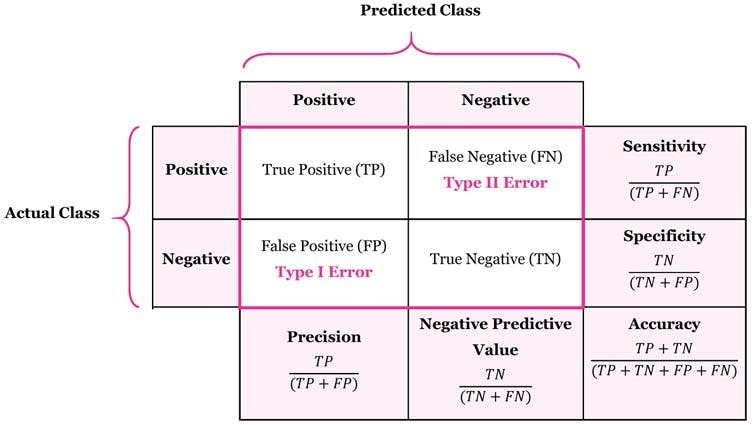
\includegraphics[width=4.53282in,height=3.52113in,alt={Confusion Matrix for binary classification}]{img/KonfusionMatrixWithMetrics.jpg}

}

\caption{\label{fig-quarto}Confusion Matrix for binary classification}

\end{figure}%

Based on the confusion matrix, the following metrics are defined:

\textbf{- Accuracy} \textbf{= (TP + TN) / (TP +TN + FP + FN) * 100\%}

Accuracy measures the percentage of all correct classifications.

\textbf{- Precision = TP / (TP + FP) * 100\%}

Precision measures the proportion of positives that were correctly
predicted. It is a measure of how sure about positive predictions one
can be.

\textbf{- Recall = TP / (TP + FN) * 100\%}

Recall (also known as sensitivity) measures the proportion of actual
positives that were predicted

correctly. It is a measure of how sure one can be about not missing any
positives.

\textbf{- F1-score = 2* (Precision * Recall) / (Precision + Recall)}

F1-score is calculated as the harmonic mean of precision and recall,
with values ranging from 0 to 1. A score close to 1 means the model
achieves both high precision and high recall, indicating that false data
(false positives and false negatives) have minimal impact. Conversely, a
low F1-score indicates the model struggles to accurately identify
positives, either missing true cases or generating many false alarms.

\chapter{Langfuse Metrics \&
Dimensions}\label{langfuse-metrics-dimensions}

\url{https://langfuse.com/?tab=metrics}

\section{Metrics:}\label{metrics}

\begin{itemize}
\item
  \textbf{Quality} is measured through

  \begin{itemize}
  \item
    user feedback,
  \item
    model-based scoring,
  \item
    human-in-the-loop scored samples or
  \item
    custom scores via SDKs/API (see scores). Quality is assessed over
    time as well as across prompt versions, LLMs and users.
  \end{itemize}
\item
  \textbf{Cost and Latency} are accurately measured and broken down by
  user, session, geography, feature, model and prompt version.
\item
  \textbf{Volume} based on the ingested traces and tokens used.
\end{itemize}

\section{Dimensions:}\label{dimensions}

\begin{itemize}
\item
  \textbf{Trace name}: differentiate between different use cases,
  features, etc. by adding a name field to your traces.
\item
  \textbf{User}: track usage and cost by user. Just add a userId to your
  traces (docs).
\item
  \textbf{Tags}: filter different use cases, features, etc. by adding
  tags to your traces.
\item
  \textbf{Release and version numbers}: track how changes to the LLM
  application affected your metrics.
\end{itemize}

For an exact definition, please refer to the metrics API docs.

\chapter{Claude-Search for „LLM Quality metrics in Claude
Code``}\label{claude-search-for-llm-quality-metrics-in-claude-code}

Aus
\textless{}\url{https://code.claude.com/docs/en/analytics}\textgreater{}

Based on the search results, the analytics page covers several LLM
quality metrics for Claude Code:

\section{Summary metrics}\label{summary-metrics}

\begin{itemize}
\item
  \textbf{Suggestion accept rate}: Percentage of times users accept
  Claude Code's code editing suggestions (Edit, Write, NotebookEdit
  tools)
\item
  \textbf{Lines of code accepted}: Total lines written by Claude Code
  that users accepted
\end{itemize}

\section{Contribution metrics (with GitHub
integration):}\label{contribution-metrics-with-github-integration}

\begin{itemize}
\item
  \textbf{PRs with CC}: Merged pull requests containing Claude
  Code-assisted code
\item
  \textbf{Lines of code with CC}: Lines across merged PRs written with
  Claude Code assistance (only ``effective lines'' with \textgreater3
  characters)
\item
  \textbf{PRs with Claude Code (\%)}: Percentage of merged PRs
  containing Claude Code-assisted code
\end{itemize}

These metrics are deliberately conservative---only lines with high
confidence in Claude Code's involvement are counted. The dashboard also
tracks adoption (daily active users, sessions) and PRs per user to
measure productivity changes.

For API customers, the Console dashboard shows

\begin{itemize}
\item
  lines accepted,
\item
  suggestion accept rate,
\item
  activity, and
\item
  spend metrics.
\end{itemize}

\chapter{DeepEval Metrics and
Features}\label{deepeval-metrics-and-features}

Aus
\textless{}\url{https://github.com/confident-ai/deepeval?tab=readme-ov-file\#-metrics-and-features}\textgreater{}

\begin{itemize}
\tightlist
\item
  Large variety of ready-to-use LLM eval metrics (all with explanations)
  powered by \textbf{ANY} LLM of your choice, statistical methods, or
  NLP models that run \textbf{locally on your machine} covering all use
  cases:
\end{itemize}

\section{Custom, All-Purpose Metrics:}\label{custom-all-purpose-metrics}

\begin{itemize}
\item
  \href{https://deepeval.com/docs/metrics-llm-evals}{G-Eval} --- a
  research-backed LLM-as-a-judge metric for evaluating on any custom
  criteria with human-like accuracy
\item
  \href{https://deepeval.com/docs/metrics-dag}{DAG} --- DeepEval's
  graph-based deterministic LLM-as-a-judge metric builder
\end{itemize}

\section{Agentic Metrics}\label{agentic-metrics}

\begin{itemize}
\item
  \href{https://deepeval.com/docs/metrics-task-completion}{Task
  Completion} --- evaluate whether an agent accomplished its goal
\item
  \href{https://deepeval.com/docs/metrics-tool-correctness}{Tool
  Correctness} --- check if the right tools were called with the right
  arguments
\item
  \href{https://deepeval.com/docs/metrics-goal-accuracy}{Goal Accuracy}
  --- measure how accurately the agent achieved the intended goal
\item
  \href{https://deepeval.com/docs/metrics-step-efficiency}{Step
  Efficiency} --- evaluate whether the agent took unnecessary steps
\item
  \href{https://deepeval.com/docs/metrics-plan-adherence}{Plan
  Adherence} --- check if the agent followed the expected plan
\item
  \href{https://deepeval.com/docs/metrics-plan-quality}{Plan Quality}
  --- evaluate the quality of the agent's plan
\item
  \href{https://deepeval.com/docs/metrics-tool-use}{Tool Use} ---
  measure quality of tool usage
\item
  \href{https://deepeval.com/docs/metrics-argument-correctness}{Argument
  Correctness} --- validate tool call arguments
\end{itemize}

\section{RAG Metrics}\label{rag-metrics}

\begin{itemize}
\item
  \href{https://deepeval.com/docs/metrics-answer-relevancy}{Answer
  Relevancy} --- measure how relevant the RAG pipeline's output is to
  the input
\item
  \href{https://deepeval.com/docs/metrics-faithfulness}{Faithfulness}
  --- evaluate whether the RAG pipeline's output factually aligns with
  the retrieval context
\item
  \href{https://deepeval.com/docs/metrics-contextual-recall}{Contextual
  Recall} --- measure how well the RAG pipeline's retrieval context
  aligns with the expected output
\item
  \href{https://deepeval.com/docs/metrics-contextual-precision}{Contextual
  Precision} --- evaluate whether relevant nodes in the RAG pipeline's
  retrieval context are ranked higher
\item
  \href{https://deepeval.com/docs/metrics-contextual-relevancy}{Contextual
  Relevancy} --- measure the overall relevance of the RAG pipeline's
  retrieval context to the input
\item
  \href{https://deepeval.com/docs/metrics-ragas}{RAGAS} --- average of
  answer relevancy, faithfulness, contextual precision, and contextual
  recall
\end{itemize}

\section{Multi-Turn Metrics}\label{multi-turn-metrics}

\begin{itemize}
\item
  \href{https://deepeval.com/docs/metrics-knowledge-retention}{Knowledge
  Retention} --- evaluate whether the chatbot retains factual
  information throughout a conversation
\item
  \href{https://deepeval.com/docs/metrics-conversation-completeness}{Conversation
  Completeness} --- measure whether the chatbot satisfies user needs
  throughout a conversation
\item
  \href{https://deepeval.com/docs/metrics-turn-relevancy}{Turn
  Relevancy} --- evaluate whether the chatbot generates consistently
  relevant responses throughout a conversation
\item
  \href{https://deepeval.com/docs/metrics-turn-faithfulness}{Turn
  Faithfulness} --- check if the chatbot's responses are factually
  grounded in retrieval context across turns
\item
  \href{https://deepeval.com/docs/metrics-role-adherence}{Role
  Adherence} --- evaluate whether the chatbot adheres to its assigned
  role throughout a conversation
\end{itemize}

\section{MCP Metrics}\label{mcp-metrics}

\begin{itemize}
\item
  \href{https://deepeval.com/docs/metrics-mcp-task-completion}{MCP Task
  Completion} --- evaluate how effectively an MCP-based agent
  accomplishes a task
\item
  \href{https://deepeval.com/docs/metrics-mcp-use}{MCP Use} --- measure
  how effectively an agent uses its available MCP servers
\item
  \href{https://deepeval.com/docs/metrics-multi-turn-mcp-use}{Multi-Turn
  MCP Use} --- evaluate MCP server usage across conversation turns
\end{itemize}

\section{Multimodal Metrics}\label{multimodal-metrics}

\begin{itemize}
\item
  \href{https://deepeval.com/docs/multimodal-metrics-text-to-image}{Text
  to Image} --- evaluate image generation quality based on semantic
  consistency and perceptual quality
\item
  \href{https://deepeval.com/docs/multimodal-metrics-image-editing}{Image
  Editing} --- evaluate image editing quality based on semantic
  consistency and perceptual quality
\item
  \href{https://deepeval.com/docs/multimodal-metrics-image-coherence}{Image
  Coherence} --- measure how well images align with their accompanying
  text
\item
  \href{https://deepeval.com/docs/multimodal-metrics-image-helpfulness}{Image
  Helpfulness} --- evaluate how effectively images contribute to user
  comprehension of the text
\item
  \href{https://deepeval.com/docs/multimodal-metrics-image-reference}{Image
  Reference} --- evaluate how accurately images are referred to or
  explained by accompanying text
\end{itemize}

\section{Other Metrics}\label{other-metrics}

\begin{itemize}
\item
  \href{https://deepeval.com/docs/metrics-hallucination}{Hallucination}
  --- check whether the LLM generates factually correct information
  against provided context
\item
  \href{https://deepeval.com/docs/metrics-summarization}{Summarization}
  --- evaluate whether summaries are factually correct and include
  necessary details
\item
  \href{https://deepeval.com/docs/metrics-bias}{Bias} --- detect gender,
  racial, or political bias in LLM outputs
\item
  \href{https://deepeval.com/docs/metrics-toxicity}{Toxicity} ---
  evaluate toxicity in LLM outputs
\item
  \href{https://deepeval.com/docs/metrics-json-correctness}{JSON
  Correctness} --- check whether the output matches an expected JSON
  schema
\item
  \href{https://deepeval.com/docs/metrics-prompt-alignment}{Prompt
  Alignment} --- measure whether the output aligns with instructions in
  the prompt template
\end{itemize}

\chapter{Microsoft Foundry Built-in evaluators
reference}\label{microsoft-foundry-built-in-evaluators-reference}

Microsoft Foundry provides a comprehensive set of built-in evaluators to
assess the quality, safety, and reliability of AI responses throughout
the development lifecycle. This reference details all available
evaluators, their purposes, required inputs, and guidance on selecting
the right evaluator for your use case. You can also create
\href{https://learn.microsoft.com/en-us/azure/foundry/concepts/evaluation-evaluators/custom-evaluators}{custom
evaluators} tailored to your specific evaluation criteria.1F{[}2{]}

\section{General purpose evaluators}\label{general-purpose-evaluators}

Evaluator

Purpose

Coherence

Measures logical consistency and flow of responses.

Fluency

Measures natural language quality and readability.

To learn more, see
\href{https://learn.microsoft.com/en-us/azure/foundry/concepts/evaluation-evaluators/general-purpose-evaluators}{General
purpose evaluators}.

\section{Textual similarity
evaluators}\label{textual-similarity-evaluators}

Evaluator

Purpose

Similarity

AI-assisted textual similarity measurement.

F1 Score

Harmonic mean of precision and recall in token overlaps between response
and ground truth.

BLEU

Bilingual Evaluation Understudy score for translation quality measures
overlaps in n-grams between response and ground truth.

GLEU

Google-BLEU variant for sentence-level assessment measures overlaps in
n-grams between response and ground truth.

ROUGE

Recall-Oriented Understudy for Gisting Evaluation measures overlaps in
n-grams between response and ground truth.

METEOR

Metric for Evaluation of Translation with Explicit Ordering measures
overlaps in n-grams between response and ground truth.

To learn more, see
\href{https://learn.microsoft.com/en-us/azure/foundry/concepts/evaluation-evaluators/textual-similarity-evaluators}{Textual
similarity evaluators}.

\section{RAG evaluators}\label{rag-evaluators}

Evaluator

Purpose

Retrieval

Measures how effectively the system retrieves relevant information.

Document Retrieval

Measures accuracy in retrieval results given ground truth.

Groundedness

Measures how consistent the response is with respect to the retrieved
context.

Groundedness Pro (preview)

Measures whether the response is consistent with respect to the
retrieved context.

Relevance

Measures how relevant the response is with respect to the query.

Response Completeness (preview)

Measures to what extent the response is complete (not missing critical
information) with respect to the ground truth.

To learn more, see
\href{https://learn.microsoft.com/en-us/azure/foundry/concepts/evaluation-evaluators/rag-evaluators}{Retrieval-augmented
Generation (RAG) evaluators}.

\section{Risk and safety evaluators}\label{risk-and-safety-evaluators}

Evaluator

Purpose

Hate and Unfairness

Identifies biased, discriminatory, or hateful content.

Sexual

Identifies inappropriate sexual content.

Violence

Detects violent content or incitement.

Self-Harm

Detects content promoting or describing self-harm.

Protected Materials

Detects unauthorized use of copyrighted or protected content.

Code Vulnerability

Identifies security issues in generated code.

Ungrounded Attributes

Detects fabricated or hallucinated information inferred from user
interactions.

Prohibited Actions (preview)

Measures an AI agent's ability to engage in behaviors that violate
explicitly disallowed actions.

Sensitive Data Leakage (preview)

Measures an AI agent's vulnerability to exposing sensitive information.

To learn more, see
\href{https://learn.microsoft.com/en-us/azure/foundry/concepts/evaluation-evaluators/risk-safety-evaluators}{Risk
and safety evaluators}.

\section{Agent evaluators}\label{agent-evaluators}

Evaluator

Purpose

Task Adherence (preview)

Measures whether the agent follows through on identified tasks according
to system instructions.

Task Completion (preview)

Measures whether the agent successfully completed the requested task
end-to-end.

Intent Resolution (preview)

Measures how accurately the agent identifies and addresses user
intentions.

Task Navigation Efficiency

Determines whether the agent's sequence of steps matches an optimal or
expected path to measure efficiency.

Tool Call Accuracy

Measures the overall quality of tool calls including selection,
parameter correctness, and efficiency.

Tool Selection

Measures whether the agent selected the most appropriate and efficient
tools for a task.

Tool Input Accuracy

Validates that all tool call parameters are correct with strict criteria
including grounding, type, format, completeness, and appropriateness.

Tool Output Utilization

Measures whether the agent correctly interprets and uses tool outputs
contextually in responses and subsequent calls.

Tool Call Success

Evaluates whether all tool calls executed successfully without technical
failures.

To learn more, see
\href{https://learn.microsoft.com/en-us/azure/foundry/concepts/evaluation-evaluators/agent-evaluators}{Agent
evaluators}.

\section{Azure OpenAI graders}\label{azure-openai-graders}

Evaluator

Purpose

Model Labeler

Classifies content using custom guidelines and labels.

String Checker

Performs flexible text validations and pattern matching.

Text Similarity

Evaluates the quality of text or determine semantic closeness.

Model Scorer

Generates numerical scores (customized range) for content based on
custom guidelines.

To learn more, see
\href{https://learn.microsoft.com/en-us/azure/foundry/concepts/evaluation-evaluators/azure-openai-graders}{Azure
OpenAI Graders}.

\section{Custom evaluators (preview)}\label{custom-evaluators-preview}

In addition to built-in evaluators, you can create custom evaluators
tailored to your specific evaluation criteria. Custom evaluators allow
you to define unique scoring logic, validation rules, and quality
metrics that align with your business requirements and
application-specific needs.\\
To learn more, see
\href{https://learn.microsoft.com/en-us/azure/foundry/concepts/evaluation-evaluators/custom-evaluators}{Custom
evaluators}.

\section{Combining evaluators}\label{combining-evaluators}

For comprehensive quality assessment, combine multiple evaluators:

\begin{itemize}
\item
  \textbf{RAG applications}: Retrieval + Groundedness + Relevance +
  Content Safety
\item
  \textbf{Agent applications}: Tool Call Accuracy + Task Adherence +
  Intent Resolution + Content Safety
\item
  \textbf{Translation applications}: BLEU + METEOR + Fluency + Coherence
\item
  \textbf{All applications}: Add risk and safety evaluators (Hate and
  Unfairness, Sexual, Violence, Self-Harm) for responsible AI practices
\end{itemize}

\section{Related content}\label{related-content}

\begin{itemize}
\item
  \href{https://learn.microsoft.com/en-us/azure/foundry/concepts/observability}{Observability
  in generative AI}
\item
  \href{https://learn.microsoft.com/en-us/azure/foundry/concepts/evaluation-evaluators/general-purpose-evaluators}{General
  purpose evaluators}
\item
  \href{https://learn.microsoft.com/en-us/azure/foundry/concepts/evaluation-evaluators/textual-similarity-evaluators}{Textual
  similarity evaluators}
\item
  \href{https://learn.microsoft.com/en-us/azure/foundry/concepts/evaluation-evaluators/rag-evaluators}{Retrieval-augmented
  Generation (RAG) evaluators}
\item
  \href{https://learn.microsoft.com/en-us/azure/foundry/concepts/evaluation-evaluators/risk-safety-evaluators}{Risk
  and safety evaluators}
\item
  \href{https://learn.microsoft.com/en-us/azure/foundry/concepts/evaluation-evaluators/agent-evaluators}{Agent
  evaluators}
\item
  \href{https://learn.microsoft.com/en-us/azure/foundry/concepts/evaluation-evaluators/azure-openai-graders}{Azure
  OpenAI Graders}
\item
  \href{https://learn.microsoft.com/en-us/azure/foundry/concepts/evaluation-evaluators/custom-evaluators}{Custom
  evaluators}
\item
  \href{https://learn.microsoft.com/en-us/azure/foundry-classic/how-to/develop/evaluate-sdk}{Evaluate
  with the Foundry SDK}
\item
  \href{https://learn.microsoft.com/en-us/azure/foundry/how-to/evaluate-generative-ai-app}{Evaluate
  generative AI apps in Foundry}
\end{itemize}

\textbf{Note:} The author created this article with assistance from AI.
\href{https://learn.microsoft.com/principles-for-ai-generated-content}{Learn
more}

\textbf{7 Key LLM Metrics to Enhance AI Reliability}

\url{https://galileo.ai/blog/llm-performance-metrics}

Conor BronsdonHead of Developer Awareness

Want to measure your LLM's performance using effective LLM performance
metrics? You're not alone. Unlike traditional ML models with clear right
or wrong answers, LLMs generate diverse outputs that require
multidimensional evaluation.

Picking the right LLM performance metrics isn't just academic---it
directly affects your model's quality and business results. The wrong
metrics lead to misguided optimization, while good eval frameworks drive
continuous improvement.

This guide explores seven key metrics to measure LLM performance in
generative AI systems.

We recently explored this topic on our Chain of Thought podcast, where
industry experts shared practical insights and real-world implementation
strategies.

\textbf{What are LLM Performance Metrics?}

LLM performance metrics are quantitative measurements used to evaluate
how well a large language model performs across various dimensions.
These metrics provide standardized ways to assess model capabilities,
identify weaknesses, and track improvements over time.

Traditional ML evaluation uses deterministic metrics like accuracy and
precision, assuming clear, correct answers exist. LLM performance
metrics are fundamentally different because these models can generate
multiple equally valid outputs for the same input.

The generative nature of LLMs creates a many-to-many relationship
between inputs and acceptable outputs. Ask ``summarize this article,''
and dozens of different summaries might be equally valid---with
different details but preserving core information.

Unlike classification models that fit into a neat confusion matrix, LLMs
need evaluation frameworks that simultaneously assess factual accuracy,
relevance, coherence, safety, creativity, and efficiency. No single
metric covers this complex landscape,
making\href{https://www.galileo.ai/blog/mastering-llm-evaluation-metrics-frameworks-and-techniques}{mastering
LLM evals} a multidimensional challenge.

\begin{enumerate}
\def\labelenumi{\arabic{enumi}.}
\tightlist
\item
  \textbf{Limitations of Traditional Metrics for Generative AI}
\end{enumerate}

Traditional metrics designed for classification tasks break down with
generative models because they assume a single correct answer exists.
LLMs work in open-ended spaces where many diverse outputs can satisfy
the same prompt.

String-matching metrics like
\href{https://www.galileo.ai/blog/bleu-metric-ai-evaluation}{BLEU} and
\href{https://www.galileo.ai/blog/rouge-ai}{ROUGE} miss semantic
equivalence, penalizing different but meaningful responses. A model
might generate a factually correct answer using a completely different
vocabulary than the reference text, getting an artificially low score
despite high quality.

These problems become acute when evaluating creative text, reasoning, or
domain-specific tasks where contextual knowledge matters. In these
cases, models might generate outputs human experts judge as excellent
but automated metrics rate poorly because they differ from references.

The following seven metrics offer a multidimensional approach to
evaluating LLM performance across operational and performance
dimensions.

\textbf{LLM Performance Metric \#1: Latency}

\href{https://www.galileo.ai/blog/understanding-latency-in-ai-what-it-is-and-how-it-works}{Latency}
measures the time between submitting a prompt and receiving the complete
response. This directly impacts user experience, especially for
interactive applications where users expect responses in milliseconds,
not seconds.

Good latency measurement analyzes performance across multiple
dimensions:

\begin{itemize}
\item
  Prompt length
\item
  Response length
\item
  Input complexity
\item
  Concurrent request load
\end{itemize}

Performance varies dramatically---some models maintain consistent speed
regardless of prompt complexity, while others slow dramatically with
longer inputs.

When optimizing latency, consider the entire request pipeline, not just
model inference. Network transmission, pre-processing, tokenization, and
post-processing all contribute to overall latency. Track each component
to find bottlenecks.

You'll face trade-offs between latency and other metrics. Techniques
that improve response quality (increased sampling temperature, larger
batch sizes) may slow responses. Set latency budgets based on specific
application needs, then optimize within those constraints.

For speed-critical applications, try
\href{https://gautam75.medium.com/streaming-llm-responses-importance-and-implementation-911b135ef541}{response
streaming},
\href{https://medium.com/@sulbha.jindal/introduction-to-llm-quantization-d274020e6ab5}{model
quantization}, and
\href{https://medium.com/@manindersingh120996/how-to-optimize-llm-inference-0076d9f3dd1b}{optimized
inference}. Response caching for common queries and request batching for
high-volume scenarios also help production deployments run faster.

Comparing your latency against competitive baseline models provides
valuable context. Understanding relative performance helps teams make
smart decisions about model selection and deployment configuration.

Galileo's comprehensive
\href{https://www.galileo.ai/blog/the-definitive-guide-to-llm-monitoring-for-ai-professionals}{LLM
monitoring} tools track latency performance across different request
types and loads, allowing teams to identify performance bottlenecks and
optimize response times. Also, Galileo provides visualizations and
alerting capabilities that help maintain latency within established
SLAs.

\textbf{LLM Performance Metric \#2: Throughput}

Throughput quantifies your LLM system's processing capacity---typically
measured in tokens per second, requests per minute, or queries per
second. This impacts system scalability, costs, and ability to handle
peak loads.

Unlike latency (which focuses on individual request speed), throughput
measures aggregate processing capability across multiple concurrent
requests. A model might have excellent single-request latency but poor
throughput with many simultaneous queries---a critical distinction for
multi-user applications.

Optimizing throughput typically involves hardware acceleration, batching
strategies, and efficient resource allocation. GPU utilization, memory
bandwidth, and parallel processing capabilities significantly impact
performance. Monitor these factors alongside top-level throughput
metrics to find optimization opportunities.

For large-scale deployments, throughput directly affects infrastructure
costs and capacity planning. Understanding throughput needs for peak and
average load scenarios helps right-size infrastructure and implement
appropriate scaling policies. Over-provisioning wastes resources;
under-provisioning risks service degradation during high demand.

Advanced optimization techniques include dynamic batch sizing (adjusting
configuration based on current load) and heterogeneous computing
(distributing processing across specialized hardware).
\href{https://medium.com/@bnjmn_marie/compression-techniques-for-llms-4eba6a6e622c}{Quantization
and model compression} can also improve throughput by reducing
computational needs.

Include stress testing in your benchmarks to understand throughput
degradation under load. Many systems perform consistently up to a
threshold, then rapidly deteriorate as resources saturate. Finding these
inflection points helps establish safe operating
\href{https://www.galileo.ai/blog/llm-parameters-model-evaluation}{LLM
parameters}.

Galileo's monitoring capabilities track processing capacity across
varying traffic conditions, helping identify bottlenecks during peak
usage periods. Teams can compare throughput metrics across model
versions to ensure optimizations actually improve real-world
performance.

\textbf{LLM Performance Metric \#3: Perplexity}

Perplexity quantifies how well a language model predicts text, measuring
the model's ``surprise'' when encountering test data. Mathematically
expressed as the exponentiated average negative log-likelihood per
token, lower perplexity indicates better prediction.

Unlike metrics that evaluate outputs against references, perplexity
directly measures predictive language modeling capability. This makes it
valuable for assessing model quality independent of specific generation
tasks, revealing fundamental language understanding.

Domain-specific perplexity evals across different text categories
(technical documentation, conversations, creative writing) reveals model
strengths and weaknesses. Establish perplexity benchmarks for relevant
domains to contextualize measurements.

While perplexity correlates with general language modeling quality, its
relationship with task-specific performance is complex. Models with
similar perplexity often show dramatically different capabilities on
tasks like summarization or question answering, limiting its usefulness
as a standalone metric.

For fine-tuned models, comparing perplexity between base and fine-tuned
versions helps quantify domain adaptation. Significant perplexity
improvements on domain-specific text indicate successful specialization,
while dramatic degradation on general text might signal catastrophic
forgetting.

\href{https://arxiv.org/pdf/2311.11509}{Token-level prediction analysis}
can identify specific linguistic patterns where models struggle. This
fine-grained analysis reveals weaknesses in handling rare vocabulary,
complex syntax, or domain-specific terminology that aggregate perplexity
figures might miss.

\href{https://docs.galileo.ai/galileo/gen-ai-studio-products/galileo-guardrail-metrics/prompt-perplexity}{Galileo
measures prompt perplexity} across different text categories and
domains, helping teams benchmark language understanding capabilities.
Perplexity visualizations show performance trends over time and across
model iterations, revealing when understanding improves or degrades for
specific content types.

\textbf{LLM Performance Metric \#4: Cross-Entropy}

Cross-entropy measures the difference between predicted token
probability distributions and actual data distributions, providing a
fundamental loss function for language model training and evals. Lower
values indicate better alignment between model predictions and targets.

Unlike perplexity, which reports an intuitive ``branching factor,''
\href{https://medium.com/ai-assimilating-intelligence/cross-entropy-in-large-language-models-llms-4f1c842b5fca}{cross-entropy}
directly quantifies prediction error in bits. This makes it useful for
comparing models across different tokenization schemes or vocabulary
sizes where perplexity comparisons might mislead.

Token-level cross-entropy analysis identifies specific vocabulary items
or linguistic constructs where models show high uncertainty or
consistent mispredictions. This granular measurement helps pinpoint
weaknesses that might be addressed through architecture adjustments,
data augmentation, or fine-tuning.

For production monitoring, track cross-entropy on representative samples
over time to detect concept drift as real-world language evolves away
from training data. Significant cross-entropy increases may signal the
need for model retraining or fine-tuning on newer data.

Domain adaptation progress can be precisely quantified through
cross-entropy reduction on target-domain text. Establish domain-specific
benchmarks and monitor improvements as adaptation techniques are
applied, using these measurements to guide fine-tuning and data
curation.

While valuable for model development and evals, cross-entropy shares
perplexity's limitations as a proxy for task-specific performance.
Models with similar scores may show dramatically different capabilities
on complex reasoning or creative generation challenges.

Galileo provides detailed cross-entropy analysis tools to identify
specific tokens and patterns where models struggle. Teams can track
cross-entropy performance across model versions and data distributions,
quickly detecting concept drift that indicates the need for model
updates.

\textbf{LLM Performance Metric \#5: Token Usage}

Token usage measures the number of tokens processed during model
inference, directly affecting operational costs and context window
efficiency. For cloud-based LLM services charging per token, this
translates directly to money spent.

Track both input and output tokens separately. Input token efficiency
focuses on prompt engineering that achieves desired results with minimal
prompt length. Output token efficiency measures how concisely the model
generates responses while maintaining quality.

Context window utilization shows the percentage of available token
capacity used by a request. Models with fixed context windows (4K, 8K,
or 16K tokens) must balance comprehensive context against token
efficiency. Monitoring this helps identify opportunities for prompt
compression or truncation.

Set token budgets based on application economics and performance
requirements. These budgets should inform prompt design guidelines,
response length parameters, and retrieval strategies. Regular token
usage audits can reveal inefficient patterns across workflows.

Advanced token optimization strategies include
\href{https://arxiv.org/abs/2403.12968}{prompt compression},
\href{https://medium.com/@stefansipinkoski/optimizing-ai-agents-with-dynamic-few-shot-prompting-585919f694cc}{efficient
few-shot example selection}, and dynamic response truncation. For
knowledge-intensive applications, efficient retrieval mechanisms that
provide only relevant context can significantly reduce token
consumption.

Token usage patterns often suggest opportunities for model rightsizing.
Applications consistently using small portions of a large context window
might benefit from smaller, more efficient models. Frequent context
window saturation might indicate the need for models with larger
capacities.

Galileo provides detailed token usage analytics across prompts and
responses, identifying inefficient patterns that drive up costs. Teams
can analyze token consumption trends by application, user segment, or
specific prompt types to optimize usage while maintaining response
quality.

\textbf{LLM Performance Metric \#6: Resource Utilization}

Resource utilization covers GPU/TPU computation, memory consumption, CPU
usage, and storage requirements. These metrics influence infrastructure
costs, deployment flexibility, and environmental impact through energy
consumption.

Track both peak and sustained resource usage patterns. Peak memory usage
determines minimum hardware requirements, while sustained computation
patterns affect energy consumption and cooling needs. Many LLMs show
spiky utilization with brief intensive computation followed by relative
idleness.

GPU memory efficiency deserves special attention as it frequently limits
deployment options. Techniques like model quantization (converting
weights from FP32 to INT8/FP16),
\href{https://arxiv.org/abs/2501.01792}{activation checkpointing}, and
\href{https://medium.com/biased-algorithms/gradient-accumulation-in-pytorch-36962825fa44}{gradient
accumulation} can significantly reduce memory requirements without
proportional performance drops.

Establish resource efficiency baselines to enable comparison across
model versions and deployment configurations. These baselines help
quantify optimization impact and identify unexpected resource
consumption that might indicate inefficiencies or memory leaks.

Advanced monitoring should include hardware-specific metrics like
GPU/TPU utilization percentage, memory bandwidth consumption, and
thermal performance. These indicators help identify specific bottlenecks
and guide hardware-aware optimization.

For multi-tenant deployments serving multiple applications or users,
resource fairness and isolation metrics become essential. Monitoring
per-tenant resource consumption helps ensure equitable service and
prevents individual workloads from degrading system performance.

Galileo tracks resource utilization metrics across compute resources,
correlating usage patterns with specific workload types. Teams gain
insights into which prompts or model configurations consume
disproportionate resources, enabling targeted optimization of high-cost
operations.

\textbf{LLM Performance Metric \#7: Error Rates}

Error rates measure system reliability through metrics like request
failures, timeouts, malformed outputs, and service disruptions. While
traditional ML models might focus only on prediction errors, LLM systems
need monitoring across the entire request lifecycle.

Categorize failures into distinct types:

\begin{itemize}
\item
  Infrastructure errors (hardware/network failures)
\item
  System errors (software crashes, memory exceptions)
\item
  Model errors (hallucinations, reasoning failures)
\item
  Integration errors (API mismatches, serialization issues)
\end{itemize}

Error correlation analysis reveals patterns in failures, identifying
specific inputs or conditions that trigger problems. Set error budgets
defining acceptable reliability thresholds, with automated alerting when
error rates approach critical levels.

For high-reliability applications, implement
\href{https://arxiv.org/pdf/2406.04313}{circuit breaker patterns} and
\href{https://medium.com/@mbneto/graceful-degradation-why-it-is-important-and-how-to-achieve-it-07f6d4a5f7d5}{graceful
degradation strategies} to maintain stability during partial failures.
These might include fallback to simpler models, cached responses, or
alternative processing when primary systems struggle.

Use structured error logging with standardized formats capturing context
information, model configurations, and environment details alongside
error descriptions. This comprehensive logging enables efficient
debugging and root-cause analysis.

Include synthetic testing with adversarial inputs specifically designed
to trigger system failures. These ``chaos engineering'' approaches
proactively identify weaknesses before they impact users, enabling
preemptive fixes rather than reactive responses.

Galileo's error detection capabilities automatically identify different
error types across requests, categorizing failures, and tracking error
rates over time. Teams can drill into specific error patterns,
understand triggering conditions, and set automated alerts for rapid
remediation.

\textbf{Enhance Your LLM Performance with Galileo}

Comprehensive LLM performance evals require integrating multiple
approaches into a coherent framework addressing both technical
performance and business requirements. Galileo provides end-to-end LLM
eval capabilities spanning the complete metrics landscape, from
operational performance to generation quality and safety, to address the
challenges of generative AI evals:

\begin{itemize}
\item
  \textbf{Data Drift Detection}: Monitors changes in data distribution
  over time, helping you identify when your model may need retraining
  due to shifts in input data patterns.
\item
  \textbf{Label Quality Assessment}: Evaluates the consistency and
  accuracy of your data labels, uncovering issues that could negatively
  impact model training and predictions.
\item
  \textbf{Model Uncertainty Metrics}: Measures the confidence of model
  predictions, allowing you to quantify uncertainty and make informed
  decisions based on prediction reliability.
\item
  \textbf{Error Analysis Tools}: Provides detailed analyses of model
  errors across different data segments, enabling targeted improvements
  where they matter most.
\item
  \textbf{Fairness and Bias Metrics}: Assesses your model for potential
  biases, ensuring fair performance across diverse user groups and
  compliance with ethical standards.
\end{itemize}

Explore how Galileo's
\href{https://docs.galileo.ai/galileo/gen-ai-studio-products/galileo-guardrail-metrics}{Guardrail
Metrics} can transform your LLM development, deployment, and eval
workflow with our complete metrics framework designed specifically for
enterprise AI teams.

\textbf{Overview of Galileo Guardrail Metrics}

\url{https://docs.galileo.ai/galileo/gen-ai-studio-products/galileo-guardrail-metrics}

Utilize Galileo's Guardrail Metrics to monitor generative AI models,
ensuring adherence to quality, correctness, and alignment with project
goals.

Understand Galileo's Guardrail Metrics in LLM Studio Galileo has built a
menu of \textbf{Guardrail Metrics} to help you evaluate, observe and
protect your generative AI applications. These metrics are tailored to
your use case and are designed to help you ensure your application
quality and behavior. The Scorer definition for each metric is listed
immediately below.

Galileo's Guardrail Metrics are a combination of industry-standard
metrics and an outcome of Galileo's in-house ML Research Team.

\textbf{Output Quality Metrics}

\begin{itemize}
\item
  \href{https://docs.galileo.ai/galileo/gen-ai-studio-products/galileo-guardrail-metrics/correctness}{Correctness}
  (Open Domain Hallucinations)
\item
  \href{https://docs.galileo.ai/galileo/gen-ai-studio-products/galileo-guardrail-metrics/instruction-adherence}{Instruction
  Adherence:} Scorers.instruction\_adherence\_plus
\item
  \href{https://docs.galileo.ai/galileo/gen-ai-studio-products/galileo-guardrail-metrics/uncertainty}{Uncertainty}
\item
  \href{https://docs.galileo.ai/galileo/gen-ai-studio-products/galileo-guardrail-metrics/ground-truth-adherence}{Ground
  Truth Adherence:} Scorers.ground\_truth\_adherence\_plus
\item
  \href{https://docs.galileo.ai/galileo/gen-ai-studio-products/galileo-guardrail-metrics/completeness/completeness-plus}{Completeness}

  \begin{itemize}
  \item
    \href{https://docs.galileo.ai/galileo/gen-ai-studio-products/galileo-guardrail-metrics/completeness/completeness-luna}{Completeness
    Luna}: Scorers.completeness\_luna
  \item
    \href{https://docs.galileo.ai/galileo/gen-ai-studio-products/galileo-guardrail-metrics/completeness/completeness-plus}{Completeness
    Plus}: Scorers.completeness\_plus
  \end{itemize}
\item
  \href{https://docs.galileo.ai/galileo/gen-ai-studio-products/galileo-guardrail-metrics/bleu-and-rouge-1}{BLEU
  and ROUGE}
\end{itemize}

\textbf{Agent Quality Metrics}

\begin{itemize}
\item
  \href{https://docs.galileo.ai/galileo/gen-ai-studio-products/galileo-guardrail-metrics/action-completion}{Action
  Completion:} Scorers.action\_completion\_plus
\item
  \href{https://docs.galileo.ai/galileo/gen-ai-studio-products/galileo-guardrail-metrics/action-advancement}{Action
  Advancement:} Scorers.action\_advancement\_plus
\item
  \href{https://docs.galileo.ai/galileo/gen-ai-studio-products/galileo-guardrail-metrics/tool-selection-quality}{Tool
  Selection Quality:} Scorers.tool\_selection\_quality\_plus
\item
  \href{https://docs.galileo.ai/galileo/gen-ai-studio-products/galileo-guardrail-metrics/tool-error}{Tool
  Error:} Scorers.tool\_errors\_plus
\end{itemize}

\textbf{RAG Quality Metrics}

\begin{itemize}
\item
  \href{https://docs.galileo.ai/galileo/gen-ai-studio-products/galileo-guardrail-metrics/context-adherence}{Context
  Adherence} (Closed Domain Hallucinations)

  \begin{itemize}
  \item
    \href{https://docs.galileo.ai/galileo/gen-ai-studio-products/galileo-guardrail-metrics/context-adherence/context-adherence-luna}{Context
    Adherence Luna}: Scorers.context\_adherence\_luna
  \item
    \href{https://docs.galileo.ai/galileo/gen-ai-studio-products/galileo-guardrail-metrics/context-adherence/context-adherence-plus}{Context
    Adherence Plus}: Scorers.context\_adherence\_plus
  \end{itemize}
\item
  \href{https://docs.galileo.ai/galileo/gen-ai-studio-products/galileo-guardrail-metrics/chunk-attribution}{Chunk
  Attribution}

  \begin{itemize}
  \item
    \href{https://docs.galileo.ai/galileo/gen-ai-studio-products/galileo-guardrail-metrics/chunk-attribution/chunk-attribution-luna}{Chunk
    Attribution Luna}: Scorers.chunk\_attribution\_utilization\_luna
  \item
    \href{https://docs.galileo.ai/galileo/gen-ai-studio-products/galileo-guardrail-metrics/chunk-attribution/chunk-attribution-plus}{Chunk
    Attribution Plus}: Scorers.chunk\_attribution\_utilization\_plus
  \end{itemize}
\item
  \href{https://docs.galileo.ai/galileo/gen-ai-studio-products/galileo-guardrail-metrics/chunk-utilization}{Chunk
  Utilization}

  \begin{itemize}
  \item
    \href{https://docs.galileo.ai/galileo/gen-ai-studio-products/galileo-guardrail-metrics/chunk-utilization/chunk-utilization-luna}{Chunk
    Utilization Luna}: Scorers.chunk\_attribution\_utilization\_luna
  \item
    \href{https://docs.galileo.ai/galileo/gen-ai-studio-products/galileo-guardrail-metrics/chunk-utilization/chunk-utilization-plus}{Chunk
    Utilization Plus}: Scorers.chunk\_attribution\_utilization\_plus
  \end{itemize}
\end{itemize}

\textbf{Input Quality Metrics}

\begin{itemize}
\tightlist
\item
  \href{https://docs.galileo.ai/galileo/gen-ai-studio-products/galileo-guardrail-metrics/prompt-perplexity}{Prompt
  Perplexity}
\end{itemize}

\textbf{Safety Metrics}

\begin{itemize}
\item
  \href{https://docs.galileo.ai/galileo/gen-ai-studio-products/galileo-guardrail-metrics/private-identifiable-information}{Input
  \& Output PII}
\item
  \href{https://docs.galileo.ai/galileo/gen-ai-studio-products/galileo-guardrail-metrics/tone}{Input
  \& Output Tone}
\item
  \href{https://docs.galileo.ai/galileo/gen-ai-studio-products/galileo-guardrail-metrics/toxicity}{Input
  \& Output Toxicity}
\item
  \href{https://docs.galileo.ai/galileo/gen-ai-studio-products/galileo-guardrail-metrics/sexism}{Input
  \& Output Sexism}
\item
  \href{https://docs.galileo.ai/galileo/gen-ai-studio-products/galileo-guardrail-metrics/prompt-injection}{Prompt
  Injection}
\end{itemize}

Looking for something more specific? You can always add your own
\href{https://docs.galileo.ai/galileo/gen-ai-studio-products/galileo-observe/how-to/registering-and-using-custom-metrics}{custom
metric}.

{[}1{]} 2060313 ISO/IEC TS 22443 CD N/A, approved for registration as
DIS {[}30.99{]}

{[}2{]} Important: Items marked (preview) in this article are currently
in public preview. This preview is provided without a service-level
agreement, and we don't recommend it for production workloads. Certain
features might not be supported or might have constrained capabilities.
For more information, see
\href{https://azure.microsoft.com/support/legal/preview-supplemental-terms/}{Supplemental
Terms of Use for Microsoft Azure Previews}.

\chapter{AI Development, MLOps, and LLMOps
Lifecycle}\label{ai-development-mlops-and-llmops-lifecycle}

\section{TODO}\label{todo}

\part{Testing AI-Based Systems}

\chapter{}\label{section-1}

\chapter{Evaluation of ML-Models and ML-based
Systems}\label{evaluation-of-ml-models-and-ml-based-systems}

The following chapters cover the evaluation of ML models and systems.
This includes the evaluation of the model itself, as well as the
evaluation of the system in which the model is embedded. The evaluation
of ML models and systems is a crucial step in the development process,
as it helps to ensure that the model and system are performing as
expected and are meeting the requirements of the stakeholders.

\chapter*{Evaluation of ML Models}\label{evaluation-of-ml-models}
\addcontentsline{toc}{chapter}{Evaluation of ML Models}

\markboth{Evaluation of ML Models}{Evaluation of ML Models}

\subsection*{Test Levels for ML models}\label{test-levels-for-ml-models}
\addcontentsline{toc}{subsection}{Test Levels for ML models}

There are two test levels that can be used to evaluate ML models: -
Input data testing and - ML model testing.

Input data testing focuses on evaluating the quality of the input data,
such as checking for missing values, outliers, and data distribution. ML
model testing focuses on evaluating the performance of the model on a
given dataset, using metrics such as accuracy, precision, recall, F1
score, and AUC-ROC.

\section{Input data testing}\label{input-data-testing}

Input data testing is important because the quality of the input data
can have a significant impact on the performance of the ML model. If the
input data is of poor quality, the model may not be able to learn
effectively and may produce inaccurate results. Therefore, it is
important to perform input data testing before training the ML model to
ensure that the data is suitable for training and that any issues with
the data are addressed.

The objective of input data testing{} is to confirm that the data used
by the MLS for training, testing, and prediction is of sufficient
quality (see 3.2). It includes reviews, statistical techniques (e.g.,
testing data for bias), EDA of the training data, and static and dynamic
testing{} of the data pipeline.

\subsection{Input Data Risks and
Mitigations}\label{input-data-risks-and-mitigations}

The following table lists examples of input data risks and corresponding
testing that could be used for risk mitigation:

Potential Risks

Possible Risk Mitigations

Defects in the training data leading to bias

Problems within the algorithm, model, or ML development framework that
introduce systemic unfairness

Testing for bias -- see 5.1.2

Training data acquired from untrustworthy sources

Data is poorly managed

Data provenance testing

Poisoned training data

A/B testing -- see 6.1.9

Data provenance testing

EDA -- see 3.2.1

Attacks as part of red teaming -- see 4.2.2

Internally inconsistent dataset

Out of range data

Wrong data types

Dataset constraint testing -- see 5.1.5

Sub-optimal feature selection

Feature testing

Imbalanced dataset due to insufficient coverage of all target classes

Skewed dataset through data augmentation

Missing data

Training data focused on a subset of all use cases

Full range of values not covered in the dataset

Data representativeness testing -- see 5.1.4

Poor labelling guidelines

Ambiguous data

Poor annotation leading to inaccurate or inconsistent labels

Label correctness testing -- see 5.1.66

Poor design or integration leading to data pipeline failures

Data quality defects compromising data pipeline outputs

Performance degradation in the operational use of the data pipeline

Security breaches or uncontrolled changes impacting the data pipeline

Data pipeline testing -- see 5.1.3

\subsection{Testing for Bias}\label{testing-for-bias}

Bias in an MLS refers to non-random, unfair differences in treatment
based on sensitive attributes like gender, age, or race, which is often
unlawful and renders the system discriminatory.

Testing for bias{} in an MLS involves understanding its potential
sources, which primarily include:

\begin{itemize}
\item
  Defects in the training data, such as unrepresentativeness, historical
  skews, or deliberate poisoning (data bias).
\item
  Defects within the algorithm, model, or development framework that
  introduce systemic unfairness, such as an algorithm using a decision
  threshold for credit scores in a loan approval system (algorithmic
  bias).
\end{itemize}

Test approaches for detecting bias include the following:

\begin{itemize}
\item
  Review{}s of the overall ML workflow, and especially the data
  preparation, to identify their potential for introducing bias.
\item
  Reviews of dataset documentation to identify and mitigate potential
  sources of unfairness by examining how the data was collected,
  annotated, and what populations are represented.
\item
  Static analysis{} of both data preparation programs and the model
  implementation code to identify anti-patterns or the mishandling of
  sensitive attributes.
\item
  EDA{} of training data by using visualization and clustering methods
  to reveal imbalanced data, skewed distributions, or anomalous
  groupings across different sensitive attributes.
\item
  Dynamic testing{} to help detect bias in an ML model by feeding a
  known unbiased and representative dataset through the system and
  analyzing its predictions for statistically significant differences in
  outcomes across various sensitive groups. This identifies bias in
  model outputs, regardless of whether the bias was introduced during
  data training or during model development.
\item
  Label correctness testing{} (see 5.1.6) to identify mislabeling that
  causes incorrect associations to be learned between attributes and
  outcomes for specific sensitive attributes.
\item
  Disparate impact analysis{}:

  \begin{enumerate}
  \def\labelenumi{\arabic{enumi}.}
  \item
    Identify sensitive attributes for the model.
  \item
    Generate counterfactuals for the sensitive attributes. (e.g.,
    example scenarios where gender is changed from male to female in a
    loan application).
  \item
    Generate model output by presenting it with the counterfactuals.
  \item
    Analyze the results of multiple tests to achieve a statistically
    significant result, which determines if changing a sensitive
    attribute causes the model results to change, signaling the presence
    of bias.
  \end{enumerate}
\end{itemize}

Note: Disparate impact analysis can also be applied to combinations of
sensitive attributes, allowing hidden bias associated with attribute
combinations to be identified. However, take care to confirm that
counterfactual examples are not unrealistic, as the model may then
respond to them rather than to any underlying bias.

\subsection{Data Pipeline Testing}\label{data-pipeline-testing}

Effective data pipeline testing{} is essential not only for confirming
the reliability and performance of data-driven systems but also for
maintaining high data quality throughout the entire ML workflow (see
3.1.2).

A layered approach is employed, beginning with~data-pipeline design
reviews during the design phase.

Component testing includes testing of data ingestion components,
transformation scripts, and sensor interfaces. This testing uses code
reviews, static analysis, and hardware-specific tests to verify reliable
data capture. Component tests validate data transformation logic, test
the implementation of data validation rules, confirm robust error
handling, and test for vulnerabilities that could be exploited to
introduce malware or poisoned data.

Component integration testing~verifies the seamless flow of data across
internal interfaces and the correct interpretation of data as it moves
through the pipeline. It detects defects arising from mismatched
interfaces or incorrect assumptions between components.~

System testing~assesses the fully assembled pipeline, beginning
with~smoke testing~to confirm basic pipeline functionality.~Functional
testing~verifies the pipeline's compliance with specified requirements,
including data transformations and data routing.~Non-functional
testing~evaluates performance under load, scalability to handle
increasing data volumes, and security measures to protect data
integrity. Fault injection testing~measures pipeline robustness by
simulating defective data inputs, assessing the system's ability to
maintain data integrity when faced with unexpected or corrupted data.
Back-to-back testing~(see 6.1.10) compares the operational pipeline
against the training pipeline to verify consistent functionality.

System integration testing verifies correct interaction between the data
pipeline and external systems or services, including data sources,
storage platforms, monitoring tools, and downstream consumers such as ML
models.

Testing in production is performed on the operational system.
Back-to-back testing verifies that performance is consistent or improved
compared to previous versions.~A/B testing~(see 6.1.9) enables
comparisons of new pipeline iterations against baselines, validating
improvements while confirming no degradation in the live data stream.
Tools can be integrated to continuously monitor and observe model
behavior, performance, and potential defects in real time.

Configuration management reviews help verify that the correct pipeline
code versions, configurations, and datasets are used across training,
testing, and production.~

Finally, the test strategies must align with the pipeline's purpose.
Training pipelines, often exploratory prototypes, have different
priorities than robust operational pipelines. The testing of training
pipelines may focus on data integrity, while operational pipeline
testing prioritizes reliability, performance, and maintainability.

\subsection{Testing for Data
Representativeness}\label{testing-for-data-representativeness}

Data representativeness testing{} determines how closely the
characteristics of the datasets used for training, validation, and
testing ML models match the real-world data that the ML model will
encounter in operation. This testing addresses various forms of
misrepresentation, including skewed datasets, missing data,
disproportionate feature distributions, inadequate coverage of
operational scenarios, and imbalanced class representation (see 5.1.1).

This testing typically includes the following steps:

1. Define the target population:

\begin{itemize}
\item
  Understand the intended use cases and operational context of the MLS
\item
  Analyze the characteristics of end users and operational environments
\item
  Identify the expected operational data distributions and critical edge
  cases by:

  \begin{itemize}
  \item
    consulting domain experts to understand real-world data patterns
  \item
    analyzing data from existing systems or similar applications
  \item
    using benchmark datasets from trusted sources (e.g., NIST, industry
    databases)
  \end{itemize}
\item
  Apply stratified sampling to the representative reference data to
  create a baseline that covers all relevant subgroups in the target
  domain
\end{itemize}

2. Analyze data characteristics:

\begin{itemize}
\item
  Apply EDA (see 3.2.1) to:

  \begin{itemize}
  \item
    training/test datasets being evaluated for representativeness
  \item
    reference dataset that represents the expected operational data
  \item
    visualize distributions through histograms, scatter plots, and other
    graphical techniques
  \end{itemize}
\item
  Examine feature relationships, and correlations in particular, to
  identify patterns that should be preserved
\item
  Identify potential anomalies, gaps, or unusual concentrations in the
  data
\end{itemize}

3. Apply statistical assessment techniques:

\begin{itemize}
\item
  Use formal statistical tests such as Chi-squared and
  Kolmogorov-Smirnov to compare distributions {[}STATS{]}
\item
  Check for data imbalances, particularly in classification problems
\item
  Verify adequate coverage of both typical scenarios and edge/boundary
  cases
\end{itemize}

Testing for data representativeness should be performed before model
training to prevent building models on unrepresentative data. After
deployment, the properties of operational input data should be
continuously monitored to detect changes that might indicate data drift
from the original training data distributions (see 6.1.7 on drift
testing).

\subsection{Dataset Constraint
Testing}\label{dataset-constraint-testing}

Dataset constraint testing{} verifies whether the data in a dataset
adheres to predefined rules or constraints. The goal is to confirm the
integrity and consistency of the data used in ML. For instance, a test
of the consistency of values in a dataset could be carried out.

Constraints on data are typically found in database schemas. A database
schema defines the structure, types, and relationships of the data.
Similarly, for ML datasets, a set of constraints can be defined that act
as a logical model of the data in the dataset, which should be satisfied
if the data are correct. There are several ways of categorizing dataset
constraints. A constraint can be applied to a single value for an
attribute, which is found in a single instance (a single-value
constraint), for example:

\begin{itemize}
\item
  Missing -- tests for missing values and missing attributes.
\item
  Range -- tests that a value is in a given range.
\item
  Type -- tests that an attribute value matches the specified type
  (e.g., that if an attribute is specified as an integer, the provided
  value is not a string or real number).
\end{itemize}

Alternatively, a constraint can apply across multiple values, typically
considering the values for a single attribute across several instances
(a multi-value constraint), for example:

\begin{itemize}
\item
  Sum -- tests that the sum of all values equals, exceeds, or does not
  exceed a specified value (e.g., the total value of all points awarded
  for a Formula 1 race cannot exceed 102, and must exceed 50.5 points).
\item
  Count -- tests that the count of all non-null values for attributes or
  instances equals, exceeds, or does not exceed a specified value.
\item
  Duplicate -- tests for identical or near identical attribute values or
  instances in a dataset and enforces a limit on how many are allowed
  (often zero).
\item
  Useful~-- tests that an attribute contains some repeated values, as if
  every entry is unique (like an ID or timestamp), typically provides no
  useful patterns to be learned for an ML model.
\item
  Outlier -- identifies any values that could be considered as
  statistical outliers.
\end{itemize}

A special form of multi-value constraint can compare different values (a
comparison constraint), for example:

\begin{itemize}
\item
  Greater Than -- tests that one value for an attribute is greater than
  a value for a second attribute (e.g., the count of lines of code for a
  program exceeds its count of lines of code with defects).
\item
  Correlate -- tests that the values for one attribute correlate with
  the values for a second attribute (e.g., all students with a marks
  attribute value at least 1.33 standard deviations above the mean also
  have a value of `A' for their grade attribute).
\end{itemize}

Testing data against the defined constraints can be performed manually.
Still, the scale of the activity and the typically large size of the
dataset would require this to be automated as part of the data pipeline.
When implemented as part of the pipeline, the tool that implements
dataset constraint testing can provide reports to data scientists (for
training data anomalies) or to operations staff (for operational data
problems).

\subsection{Label Correctness Testing}\label{label-correctness-testing}

Data label correctness{} is essential in supervised learning. Inaccurate
or inconsistent labels directly undermine the performance and
generalization of ML models.

Common approaches to data label correctness testing include:

\begin{itemize}
\item
  Expert Review: Domain experts or trained annotators manually review a
  sample of labelled data. They evaluate label accuracy using their
  domain knowledge and guidelines.
\item
  Multiple Annotation{}: Data points are independently labelled by
  multiple annotators and compared using a form of back-to-back testing
  (see 6.1.10). Disagreements highlight defects that need investigation
  and resolution. The inter-annotator agreement (IAA) can be measured
  using metrics such as Cohen's Kappa or simple percentage agreement
  {[}STATS{]}. Low IAA scores can indicate defects in labelling
  guidelines, ambiguous data, or poor annotation.
\item
  Risk-Based Prioritization for Review and Annotation: Both expert
  reviews and multiple annotations can be focused using a risk-based
  approach to identify samples for review and multiple annotations.
  Prioritization can be based on the likelihood of mislabeling, such as
  with ambiguous data points (e.g., it is unclear to which category they
  belong or are near a boundary between classes), and the data that is
  most likely to impact the application's success or safety.
\item
  Data Distribution Analysis: When comparable datasets exist, comparing
  the label distribution of the dataset under test to similar datasets
  can reveal anomalies and potentially incorrect labels.
\item
  Automated Rule-Based Tests: Automated tests can be implemented based
  on predefined label rules or constraints for certain tasks. For
  instance, verifying that bounding boxes (rectangles used to locate
  objects in images) do not overlap or extend beyond image boundaries.
\item
  Model Loss Analysis: Data points exhibiting high loss during model
  training -- meaning the model's predictions for these points deviate
  substantially from their true labels -- can indicate mislabeling. High
  loss reflects significant error, indicating the model struggles to
  learn the assigned label and pointing to a potential defect.
\item
  Model Confidence Score Analysis: Data points with low prediction
  confidence from a trained model may be mislabeled, ambiguous, or lie
  outside the model's training data distribution.
\end{itemize}

Using a combination of approaches is often most effective. For example,
expert reviews are valuable in establishing clear labelling guidelines
early on. IAA scores from multiple annotations can then refine the
labelling process. Subsequently, model-based approaches can further
identify potential label defects as the model continues to develop.

\subsection{Hands-on Exercise: Input Data
Testing}\label{hands-on-exercise-input-data-testing}

For a given dataset (e.g., structured, tabular data), perform input data
testing for things like missing data, duplicate data, and outliers.

\subsection{ML Model Testing}\label{ml-model-testing}

Testing ML models is different from testing traditional software.
Traditional software testing focuses on verifying that the software
behaves as expected for a given set of inputs and outputs. In contrast,
testing ML models involves evaluating the performance of the model on a
given dataset, and comparing it to a baseline or to other models. This
is because ML models are often probabilistic in nature, and their
performance can vary depending on the data they are trained on and the
data they are tested on.

The evaluation of ML models is typically done using a set of metrics
that measure the performance of the model on a given dataset. These
metrics can be used to compare different models and to select the best
model for a given task. Some common metrics for evaluating ML models
include accuracy, precision, recall, F1 score, and area under the ROC
curve (AUC-ROC) (see Section~\ref{sec-metrics-for-classification}).

\emph{TBD: add more details on evaluation of ML models, including
different types of metrics, how to interpret them, and how to use them
for model selection.}

\chapter{Evaluation of ML-based
Systems}\label{evaluation-of-ml-based-systems}

The evaluation of ML-based systems is more complex than the evaluation
of ML models, as it involves not only the performance of the model, but
also the performance of the system as a whole. This includes factors
such as the integration of the model into the system, the user
experience, and the overall functionality of the system. The evaluation
of ML-based systems typically involves a combination of quantitative and
qualitative methods, including user testing, usability testing, and
field testing.

\section{Test Levels for ML-based
Systems}\label{test-levels-for-ml-based-systems}

There are several testing methods that can be used to evaluate ML-based
systems, including:

\begin{itemize}
\item
  \textbf{Unit testing}: testing individual components of the system,
  such as the ML model, to ensure that they are functioning correctly.
\item
  \textbf{Integration testing}: testing the integration of the ML model
  with other components of the system to ensure that they are working
  together as expected.
\item
  \textbf{System testing}: testing the entire system to ensure that it
  meets the requirements and performs as expected in real-world
  conditions.
\item
  \textbf{User acceptance testing}: testing the system with end-users to
  ensure that it meets their needs and is usable.
\end{itemize}

\subsection{Adversarial Testing}\label{adversarial-testing}

\textbf{What is Adversarial Testing?}

Adversarial testing{} is a testing method that involves intentionally
introducing adversarial examples to the ML model to evaluate its
robustness and security. Adversarial examples are inputs that are
designed to deceive the model into making incorrect predictions.

\textbf{Why to Perform Adversarial Testing?} Adversarial testing is
important because it helps to identify vulnerabilities in the ML model
and to improve its robustness against attacks. Adversarial examples can
be used to test the model's ability to generalize to new and unseen
data, and to identify potential weaknesses in the model that could be
exploited by attackers. By performing adversarial testing, developers
can improve the security and reliability of the ML model, and ensure
that it is able to perform well in real-world conditions where
adversarial attacks may be present.

\textbf{When to Perform Adversarial Testing?} Adversarial testing should
be performed during the development and testing phases of the ML model,
as well as during the deployment phase. It is important to perform
adversarial testing early in the development process to identify
vulnerabilities in the model and to improve its robustness against
attacks. Additionally, adversarial testing should be performed regularly
during the deployment phase to ensure that the model remains secure and
robust against new types of attacks.

\textbf{How to Perform Adversarial Testing?}

Adversarial testing can be performed using techniques such as:\\
- \emph{FGSM (Fast Gradient Sign Method)}: a method that generates
adversarial examples by adding small perturbations to the input data in
the direction of the gradient of the loss function. - \emph{PGD
(Projected Gradient Descent)}: an iterative method that generates
adversarial examples by repeatedly applying the FGSM method and
projecting the perturbed input back onto a specified constraint set. -
\emph{CW (Carlini \& Wagner)}: a method that generates adversarial
examples by optimizing a loss function that combines the model's output
and the distance between the original input and the adversarial example.

\emph{TBD: add more details on evaluation of ML-based systems, including
different types of evaluation methods, how to design and conduct
evaluations, and how to interpret the results.}

\chapter{German: Praktische Übungen zum Buch
``KI-Testen''}\label{german-praktische-uxfcbungen-zum-buch-ki-testen}

Das Repository
\href{https://github.com/KI-Testen/Uebungen/tree/main}{KI-Übungen}
enthält das Begleitmaterial und praktische Übungen zum Buch
``\href{https://dpunkt.de/produkt/basiswissen-ki-testen/}{\textbf{Basiswissen
KI-Testen} - Qualität von und mit KI-basierten Systemen}'' aus dem
\textbf{dpunkt.Verlag}, ISBN 978-3-86490-947-4. Die Übungen sind so
konzipiert, dass sie von jedem mit einem Laptop oder PC durchgeführt
werden können, der über grundlegende Kenntnisse in Python und JupyterLab
verfügt.

Die folgenden Abschnitte sind eine 1:1 Kopie aus dem RTepository.

Um die Übungen selbst auf \emph{deinem eigenen Laptop oder PC}
durchführen zu können, benötigst du folgendes: * Einen Laptop oder PC
(ein Smartphone oder Tablet ist eher unpraktisch). * Eine Installation
von Python auf deinem Computer (sie
\hyperref[2.-Installation-von-python]{Punkt 2 unten}). * Grundkenntnisse
in der
\href{https://tutorial.djangogirls.org/de/python_introduction}{Programmiersprache
Python} * Grundkenntnisse in der
\href{https://jupyter-tutorial.readthedocs.io/de/latest/index.html}{Benutzung
von JupyterLab}

\section{1. Download des
Übungsmaterials}\label{download-des-uxfcbungsmaterials}

\begin{itemize}
\tightlist
\item
  Lade von der GitHub-Seite
  \href{https://github.com/KI-Testen/Uebungen}{KI-Testen - Übungen} das
  gesamte Repository als ZIP-Datei (Code (grüner Button) \textgreater{}
  Download ZIP)
\item
  Entpacke die ZIP in ein Verzeichnis deiner Wahl.
\end{itemize}

\section{2. Installation von Python, ML-Paketen und
JupyterLab}\label{installation-von-python-ml-paketen-und-jupyterlab}

\begin{itemize}
\tightlist
\item
  Als erstes musst du, wenn nicht schon vorhanden,
  \href{Einstieg_Vorbereitung/Installation_Python.md}{Python
  installieren}.
\item
  Ist Python installiert, geht es mit der
  \href{Einstieg_Vorbereitung/Installation_Pakete.md}{Installation der
  Python-Pakete} weiter
\item
  Zum Schluss ist die
  \href{Einstieg_Vorbereitung/Installation_JupyterLab.md}{Installation
  von JupyterLab} an der Reihe.
\end{itemize}

\section{3. Los geht's: Starten von
JupyterLab}\label{los-gehts-starten-von-jupyterlab}

Von nun ab kannst du JupyterLab per Doppelklick auf:
\texttt{04\_starte\_jupyterlab.cmd} starten. Als erstes öffnet sich ein
Kommandozeilenfenster mit dem Titel ``JupyterLab Server''.

Nach dem Start des CMD-Skriptes startet zudem dein Browser und öffnet
eine Seite, die sich mit dem JupyterLab-Server (localhost:8888/lab/tree)
verbindet, der im Kommandozeilenfenster läuft - lasse dieses also im
Hintergrund weiter laufen!

Wenn du einen bestimmten Browser bevorzugst, kannst du die Datei
\texttt{04\_starte\_jupyterlab.cmd} editieren und eine der drei per
\texttt{::} auskommentierten Zeilen durch das Entfernen des \texttt{::}
aktivieren und so deinen Lieblingsbrowser festlegen.

\begin{figure}[H]

{\centering \pandocbounded{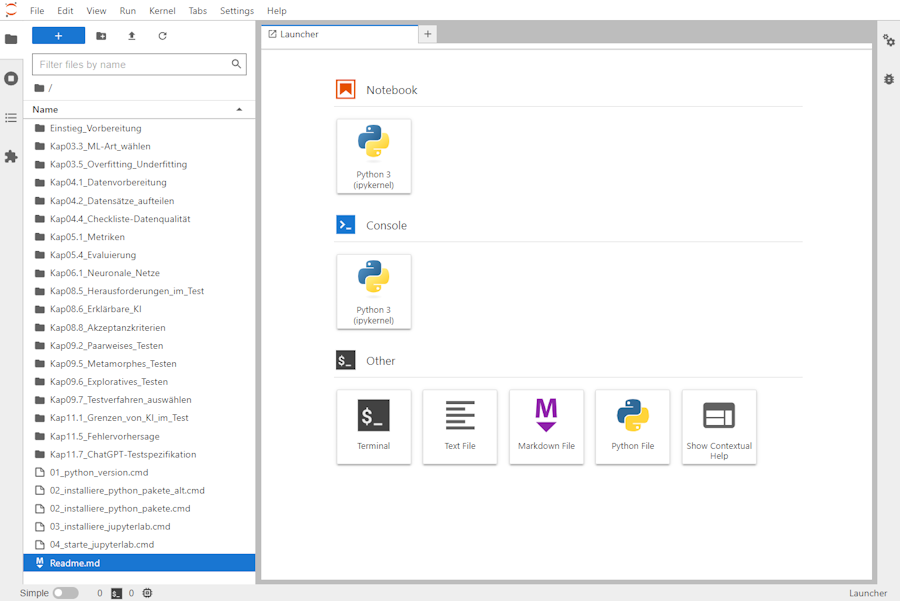
\includegraphics[keepaspectratio]{Einstieg_Vorbereitung/jupyterlab_snapshot01_blanko.png}}

}

\caption{snapshot von JupyterLab}

\end{figure}%

\begin{itemize}
\tightlist
\item
  \emph{Diese} Anleitung (die du gerade liest) kannst du dir ansehen,
  wenn du mit der rechten Maustaste auf \texttt{Readme.md} klickst und
  \emph{Open With \textgreater{} Markdown Preview} auswählst.
\end{itemize}

\section{4. Mit den Aufgaben loslegen}\label{mit-den-aufgaben-loslegen}

\emph{Hinweis:} Wir empfehlen dir, die Aufgaben nicht ohne eine gewisse
Vorbereitung durch den entsprechenden Abschnitt im Buch zu beginnen.

\emph{Außerdem:} Es ist gut, wenn du einfache Grundkenntnisse in Python
als Programmiersprache mitbringst, und dich mit der Bedienung von
\textbf{JupyterLab} und \textbf{Juypter Notebooks} schon etwas vertraut
gemacht hast
(\hyperref[Praktische-ux5cux25C3ux5cux259Cbungen-zum-Buch-ux5cux2522KI-Testenux5cux2522]{siehe
oben}).

Zum Bearbeiten einer Aufgabe - zum Beispiel zum Abschnitt 3.3: * öffnest
du in JupyterLab per Doppel-Click das Verzeichnis
\texttt{Kap03.3\_ML-Art-wählen} und * öffnest das Notebook
\texttt{Übung\_...} ebenfalls per Doppel-Click.

und schon kann's losgehen!

\section*{Lizenzbedingungen}\label{lizenzbedingungen}
\addcontentsline{toc}{section}{Lizenzbedingungen}

\markright{Lizenzbedingungen}

\textbf{der Inhalte \emph{dieses} GitHub-Repos (Notebooks, Grafiken,
Code\ldots):}

\pandocbounded{
\includegraphics[keepaspectratio,alt={cc-license}]{index_files/mediabag/Einstieg_Vorbereitung/cc-by-nc-sa.pdf}}
CC BY-NC-SA 4.0 (https://creativecommons.org/licenses/by-nc-sa/4.0/)

\textbf{der genutzten Werkzeuge und Daten:}

\begin{itemize}
\tightlist
\item
  pyhton: \href{https://docs.python.org/3/license.html}{PSF License} -
  GPL-kompatibel
\item
  jupyterlab:
  \href{https://jupyterlab.readthedocs.io/en/latest/api/index.html?highlight=license\#md:license}{BSD
  License}
\item
  iris dataset: \href{https://archive.ics.uci.edu/dataset/53/iris}{CC-BY
  4.0, donated by R. A. Fisher}
\item
  tensorflow playground:
  \href{https://github.com/tensorflow/playground/blob/master/LICENSE}{Apache
  License}
\item
  lime: Copyright © 2016, Marco Tulio Correia Ribeiro
  \href{https://de.wikipedia.org/wiki/BSD-Lizenz}{BSD-2-Clause License}
\item
  shap: Copyright © 2018, Scott Lundberg
  \href{https://en.wikipedia.org/wiki/MIT_License}{MIT License}
\item
  pict: Copyright © Microsoft Corporation
  \href{https://en.wikipedia.org/wiki/MIT_License}{MIT License}
\item
  chatGPT: OpenAI \href{https://openai.com/policies/terms-of-use}{Terms
  of Use}
\item
  \href{http://creativecommons.org/licenses/by/4.0/}{OpenML}
  \href{https://opensource.org/licenses/BSD-3-Clause}{sowie BSD-3}
\end{itemize}

\chapter{}\label{section-2}

\chapter{}\label{section-3}

\part{AI Testing in Practice}

\chapter{}\label{section-4}

\chapter{}\label{section-5}

\part{Appendices}

\chapter{An Introduction to Quarto}\label{an-introduction-to-quarto}

Quarto is a powerful document authoring system that enables you to
create reports, presentations, books, and more from a single source
file. It supports multiple output formats, including HTML, PDF, and
DOCX, making it easy to share your work in the format that best suits
your audience. Quarto is built on top of R Markdown, which means you can
include executable code chunks in your documents. This allows you to
create dynamic reports that automatically update when the underlying
data changes.

\section{What is Quarto?}\label{what-is-quarto}

Quarto is an open-source scientific and technical publishing system
built on Pandoc\footnote{Pandoc is a tool that converts documents to
  different formats. Quarto leverages it to convert markdown to a
  variety of output formats.}. It provides a unified authoring framework
for reproducible data science, combining code, results, and narrative to
produce outputs like HTML, PDF, Word, and more in a seamless manner. A
few of the key features of Quarto that are applicable to Quarto users at
any level are listed below:

\begin{enumerate}
\def\labelenumi{\arabic{enumi}.}
\item
  \textbf{Markdown authoring}: Quarto documents are authored using
  \textbf{markdown}, a straightforward plain text format that allows you
  to add formatting elements to plain text documents using a simple
  syntax.
\item
  \textbf{Code integration}: Quarto coordinates the execution of knitr,
  Jupyter or Observable to embed code and output from various languages,
  including Python, R, Julia, and JavaScript.
\item
  \textbf{Technical writing extensions}: Quarto markdown adds syntax for
  technical writing that covers features like cross-references,
  sub-figures, layout panels, hoverable citations and footnotes, and
  more.
\item
  \textbf{Project system}: Quarto provides a project system for managing
  groups of documents with shared options to produce aggregate output
  such as manuscripts, websites, and books.
\item
  \textbf{Editor compatibility:} Quarto supports authoring in various
  editors and notebooks, including JupyterLab, RStudio, and VS Code.
  Many of these editors offer a visual markdown editor that is
  specifically designed to work well with Quarto, providing a productive
  writing interface for composing long-form documents.
\end{enumerate}

The best place to learn about Quarto and explore its capabilities, aside
from this book, is \href{https://quarto.org/}{quarto.org}.

Quarto is available under the \href{https://quarto.org/license.html}{MIT
license}.

Sometimes when we say ``Quarto'' we mean ``a Quarto document'', i.e., a
plain-text Quarto markdown file with the extension \texttt{.qmd}. And
sometimes when we say ``Quarto'' we mean the Quarto Command Line
Interface (CLI), which can render \texttt{.qmd} files as well as
\texttt{.ipynb} (Jupyter Notebook), \texttt{.Rmd} (R Markdown), and
\texttt{.md} (Markdown) files.

\section{Installation}\label{installation}

The Quarto CLI is the tool you need to render Quarto documents.
Specifically, it gives you the command \texttt{quarto\ render}. You can
download the latest release version of the Quarto CLI at
\href{https://quarto.org/docs/get-started/}{https://quarto.org/docs/get-started}
and install it.

\begin{tcolorbox}[enhanced jigsaw, arc=.35mm, bottomrule=.15mm, bottomtitle=1mm, breakable, colback=white, colbacktitle=quarto-callout-note-color!10!white, colframe=quarto-callout-note-color-frame, coltitle=black, left=2mm, leftrule=.75mm, opacityback=0, opacitybacktitle=0.6, rightrule=.15mm, title=\textcolor{quarto-callout-note-color}{\faInfo}\hspace{0.5em}{Note}, titlerule=0mm, toprule=.15mm, toptitle=1mm]

You can also download development versions of Quarto at
\url{https://quarto.org/docs/download/prerelease.html} however note that
pre-release builds are intended for testing purposes, and are not
recommended for general use.

\end{tcolorbox}

\section{Tools for authoring}\label{tools-for-authoring}

You do not need a specific tool for authoring and rendering Quarto
documents. You can author Quarto documents in any plain text editor and
render them with the \texttt{quarto\ render} command in your computer's
terminal.

However we recommend using an integrated development environment (IDE)
when working with Quarto as they can enhance your authoring experience.
Some compelling reasons for using an IDE with Quarto include preview and
live rendering features that allow you to see how your content will look
as you write it, syntax highlighting, project management features,
version control integration, debugging tools, and efficiency and
productivity features like snippets, templates, and keyboard shortcuts.
Additionally, most modern IDEs offer intelligent code assistance,
auto-completion, and error highlighting which can help you quickly find
the right syntax and catch errors.

In the next section we go into further detail about using Quarto in VS
Code, and Jupyter Lab.

\section{Working with Quarto in VS
Code}\label{working-with-quarto-in-vs-code}

VS Code is a popular code editor that supports a wide range of
programming languages and file formats, including Quarto documents. To
work with Quarto in VS Code, you can install the ``Quarto'' extension
from the VS Code marketplace. This extension provides features such as
syntax highlighting, code snippets, and live preview for Quarto
documents. Once you have the extension installed, you can create a new
Quarto document by selecting ``File'' \textgreater{} ``New File'' and
saving it with a \texttt{.qmd} extension. You can then start writing
your Quarto document using markdown syntax and code chunks. To render
your Quarto document, you can use the command palette (Ctrl+Shift+P) and
select ``Quarto: Render Document'' or use the keyboard shortcut
(Ctrl+Shift+R).\\
This will generate the output file in the same directory as your source
file, with the appropriate extension based on the output format you
specified in your document.

\section{Working with Quarto in Jupyter
Lab}\label{working-with-quarto-in-jupyter-lab}

Jupyter Lab is an interactive development environment that allows you to
create and share documents that contain live code, equations,
visualizations, and narrative text. To work with Quarto in Jupyter Lab,
you can install the ``Quarto'' extension from the Jupyter Lab extension
manager. This extension provides features such as syntax highlighting,
code snippets, and live preview for Quarto documents within the Jupyter
Lab interface. Once you have the extension installed, you can create a
new Quarto document by selecting ``File'' \textgreater{} ``New''
\textgreater{} ``Quarto Document'' from the Jupyter Lab menu. This will
create a new \texttt{.qmd} file in your Jupyter Lab workspace where you
can start writing your Quarto document using markdown syntax and code
chunks. To render your Quarto document, you can use the command palette
(Ctrl+Shift+C) and select ``Quarto: Render Document'' or use the
keyboard shortcut (Ctrl+Shift+R).\\
This will generate the output file in the same directory as your source
file, with the appropriate extension based on the output format you
specified in your document.

\section{Using Quarto Markdown}\label{using-quarto-markdown}

Quarto markdown is an extension of standard markdown that includes
additional syntax for technical writing and reproducible research. In
addition to the standard markdown syntax for formatting text, Quarto
markdown includes features such as cross-references, sub-figures, layout
panels, hoverable citations and footnotes, and more. These features
allow you to create more complex and structured documents that are
well-suited for scientific and technical writing.

\section{Writing content}\label{sec-writing}

Beyond the document header and executable code cells, the content of a
Quarto document is written in markdown. But not just any flavor of
markdown, Quarto's own flavor called \textbf{Quarto markdown}. In this
chapter, you'll learn just enough about Quarto markdown to get you
writing simple documents right away. We'll tease you with some of the
rich content you can create with Quarto markdown, but delay a
comprehensive coverage of things like equations, cross-references,
citations, callouts, figures and tables to Chapter~\ref{sec-authoring}.

\subsection{Basics}\label{basics}

Markdown is a plaintext syntax for describing document structure. Here's
some example markdown in a Quarto document:

\begin{codelisting}

\caption{\texttt{document.qmd}}

\begin{Shaded}
\begin{Highlighting}[]
\FunctionTok{\#\#\# My First Section}

\NormalTok{This is the first paragraph with some **bold text** and *italic text*.}
\NormalTok{You can also include }\InformationTok{\textasciigrave{}code\textasciigrave{}}\NormalTok{ to show function names or variables.}

\NormalTok{Here\textquotesingle{}s a second paragraph with a }\CommentTok{[}\OtherTok{link to Quarto}\CommentTok{](https://quarto.org)}\NormalTok{.}
\NormalTok{You might also want to use *italic text* for emphasis.}
\end{Highlighting}
\end{Shaded}

\end{codelisting}

Markdown is a popular format, so the syntax above may be familiar.
You've likely used it if you've opened an issue on Github, or formatted
some text in a Discord post. However, as markdown's popularity has
grown, so has the number of variants, or flavors, of the syntax.

The example above illustrates components of markdown syntax that are
common across many markdown variants:

\begin{itemize}
\item
  Headings: text prefaced by one or more hashes (\texttt{\#}),
  surrounded by blank lines.
\item
  Paragraphs: text separated by blank lines.
\item
  Bold: text surrounded by \texttt{**}
\item
  Italic: text surrounded by \texttt{*}
\item
  Code: text surrounded by \texttt{\textasciigrave{}}
\item
  Links: text inside square brackets (\texttt{{[}{]}}) followed by a URL
  in parentheses (\texttt{()})
\end{itemize}

When rendered the structure described by markdown is translated to the
relevant components in the target format, e.g.~HTML tags for
\texttt{format:\ html}, or Typst functions for \texttt{format:\ typst}.

TODO: screenshots of rendered output

\subsection{Features of Quarto
markdown}\label{features-of-quarto-markdown}

Describing basic document structure, like headings and paragraphs, and
simple text formatting is enough to get started with Quarto. But you may
soon be looking for richer content like tables, figures, code blocks,
citations, and cross-references. Adding these components is a matter of
adding the appropriate Quarto markdown. As a teaser, here's an example
contains a callout and a cross-reference:

\begin{codelisting}

\caption{\texttt{document.qmd}}

\begin{Shaded}
\begin{Highlighting}[]
\NormalTok{::: \{.callout{-}caution\}}
\FunctionTok{\#\# Preliminary Data}

\NormalTok{These results are preliminary and subject to change. Use caution when drawing conclusions.}
\NormalTok{:::}

\NormalTok{@fig{-}response shows a notable decline in the survey response rate over time.}

\AlertTok{![Survey response rate over time](images/response.png)}\NormalTok{\{\#fig{-}response\}}
\end{Highlighting}
\end{Shaded}

\end{codelisting}

It is important to remember that Quarto markdown is a specific flavor of
markdown---although it shares much of its syntax with other variants you
shouldn't expect a component of any arbitrary markdown variant to work
with Quarto.

The above example illustrates two pieces of syntax you'll see often in
Quarto markdown that you might not have seen in other variants:

\begin{itemize}
\item
  Attributes: additional metadata for a component specified inside curly
  braces, e.g the \texttt{\{\#fig-repsonse\}} on the image. You'll see
  lots of examples in Chapter~\ref{sec-authoring}, and can specifically
  learn more in Tip~\ref{tip-attributes}.
\item
  Fenced divs: blocks of content inside colon delimited sections, often
  with attributes attached, e.g.~the callout:

\begin{Shaded}
\begin{Highlighting}[]
\NormalTok{::: \{.callout{-}caution\}}
\NormalTok{Content}
\NormalTok{:::}
\end{Highlighting}
\end{Shaded}

  Fenced divs are used in Quarto to implement lots of different block
  level treatments: callouts, figure or table panels, and complex
  layouts.
\end{itemize}

Chapter~\ref{sec-authoring} covers the most useful features of Quarto
markdown in more detail.

\subsection{Things to watch out for}\label{things-to-watch-out-for}

\subsection{White space matters
(sometimes)}\label{white-space-matters-sometimes}

You can often ignore whitespace when you are writing Quarto markdown.
For example, extra spaces inline with text are ignored, as are newlines
within a paragraph. That is, the following markdown snippets are
equivalent:

\begin{figure}

\begin{minipage}[t]{0.50\linewidth}

\begin{Shaded}
\begin{Highlighting}[]
\NormalTok{A sentence  with   weird     spacing.   And    another.}
\NormalTok{This is on a new line.}
\end{Highlighting}
\end{Shaded}

\end{minipage}%
%
\begin{minipage}[t]{0.50\linewidth}

\begin{Shaded}
\begin{Highlighting}[]
\NormalTok{A sentence with weird spacing. And another. This is on a new line.}
\end{Highlighting}
\end{Shaded}

\end{minipage}%

\end{figure}%

However, there are some places white space is important:

\begin{itemize}
\item
  \textbf{Blank lines}: you must have a blank line before the items in a
  list, and before a code block or cell. Without the blank line, Quarto
  won't identify the component correctly, so you'll get list items that
  all appear on a single line, or a code block syntax (the
  \texttt{\textasciigrave{}\textasciigrave{}\textasciigrave{}}) showing
  up in the rendered document.
\item
  \textbf{Indentation}: items in a list need consistent indentation.
  Problems with indentation most often occur when an item has multiple
  paragraphs, or contains something like a code block. You'll notice
  that your items don't seem properly aligned in the output (usually not
  enough indentation), or something suddenly looks like a code block
  (usually too much indentation).
\end{itemize}

If your content isn't rendering as expected, double-check your use of
whitespace.

\subsection{The difference between code blocks and code
cells}\label{the-difference-between-code-blocks-and-code-cells}

There is a distinction between:

\begin{itemize}
\item
  \textbf{Code cells}, sometimes also called \textbf{code chunks}, are
  code that will be executed and replaced with computational output.
  Code cells use the syntax:

\begin{Shaded}
\begin{Highlighting}[]
\InformationTok{\textasciigrave{}\textasciigrave{}\textasciigrave{}\{r\}}
\CommentTok{\# Code to be executed}
\InformationTok{\textasciigrave{}\textasciigrave{}\textasciigrave{}}
\end{Highlighting}
\end{Shaded}

  Code cells are the subject of the next chapter, \textbf{?@sec-code}
\item
  \textbf{Code blocks} are code that should be syntax highlighted but
  simply displayed, not executed. Code blocks use the syntax:

\begin{Shaded}
\begin{Highlighting}[]
\InformationTok{\textasciigrave{}\textasciigrave{}\textasciigrave{}\{.r\}}
\CommentTok{\# Code to be displayed}
\InformationTok{\textasciigrave{}\textasciigrave{}\textasciigrave{}}
\end{Highlighting}
\end{Shaded}

  Or the syntax:

\begin{Shaded}
\begin{Highlighting}[]
\InformationTok{\textasciigrave{}\textasciigrave{}\textasciigrave{} r}
\CommentTok{\# Code to be displayed}
\InformationTok{\textasciigrave{}\textasciigrave{}\textasciigrave{}}
\end{Highlighting}
\end{Shaded}

  You'll can more about code blocks in Section~\ref{sec-code-blocks}.
\end{itemize}

The syntax difference, as little as a \texttt{.}, means it is easy to
mistake one for the other in your document. However, the differences in
behavior are huge---code cells are handled by the computational engine,
code blocks are not. When you are reading examples, or trouble-shooting
your own documents, keep that distinction in mind and be wary of trying
to apply solutions for code blocks to code cells and vice versa.

\section{Wrap Up}\label{wrap-up}

In this chapter, you got a high-level overview of Quarto and how to get
started with it. You learned about the Quarto CLI and how to install it,
and about using Quarto in VS Code and Jupyter Lab. You also got a brief
introduction to Quarto markdown, the syntax used to write content in
Quarto documents, and some of the features and quirks of that syntax.

\chapter{Using Jupyter Notebooks in Quarto
Books}\label{using-jupyter-notebooks-in-quarto-books}

This is a Jupyter Notebook embedded in a Quarto book. You can write
code, run it, and see the results directly in the book.

\section{Overview}\label{overview}

Quarto can render Jupyter notebooks represented as plain text (.qmd) or
as a normal notebook file (.ipynb). One benefit of using .ipynb is that
you can use
\href{https://jupyterlab.readthedocs.io/en/stable/}{JupyterLab} as your
editor.

Here is the ``Hello, Quarto'' example from the homepage inside
JupyterLab:

\pandocbounded{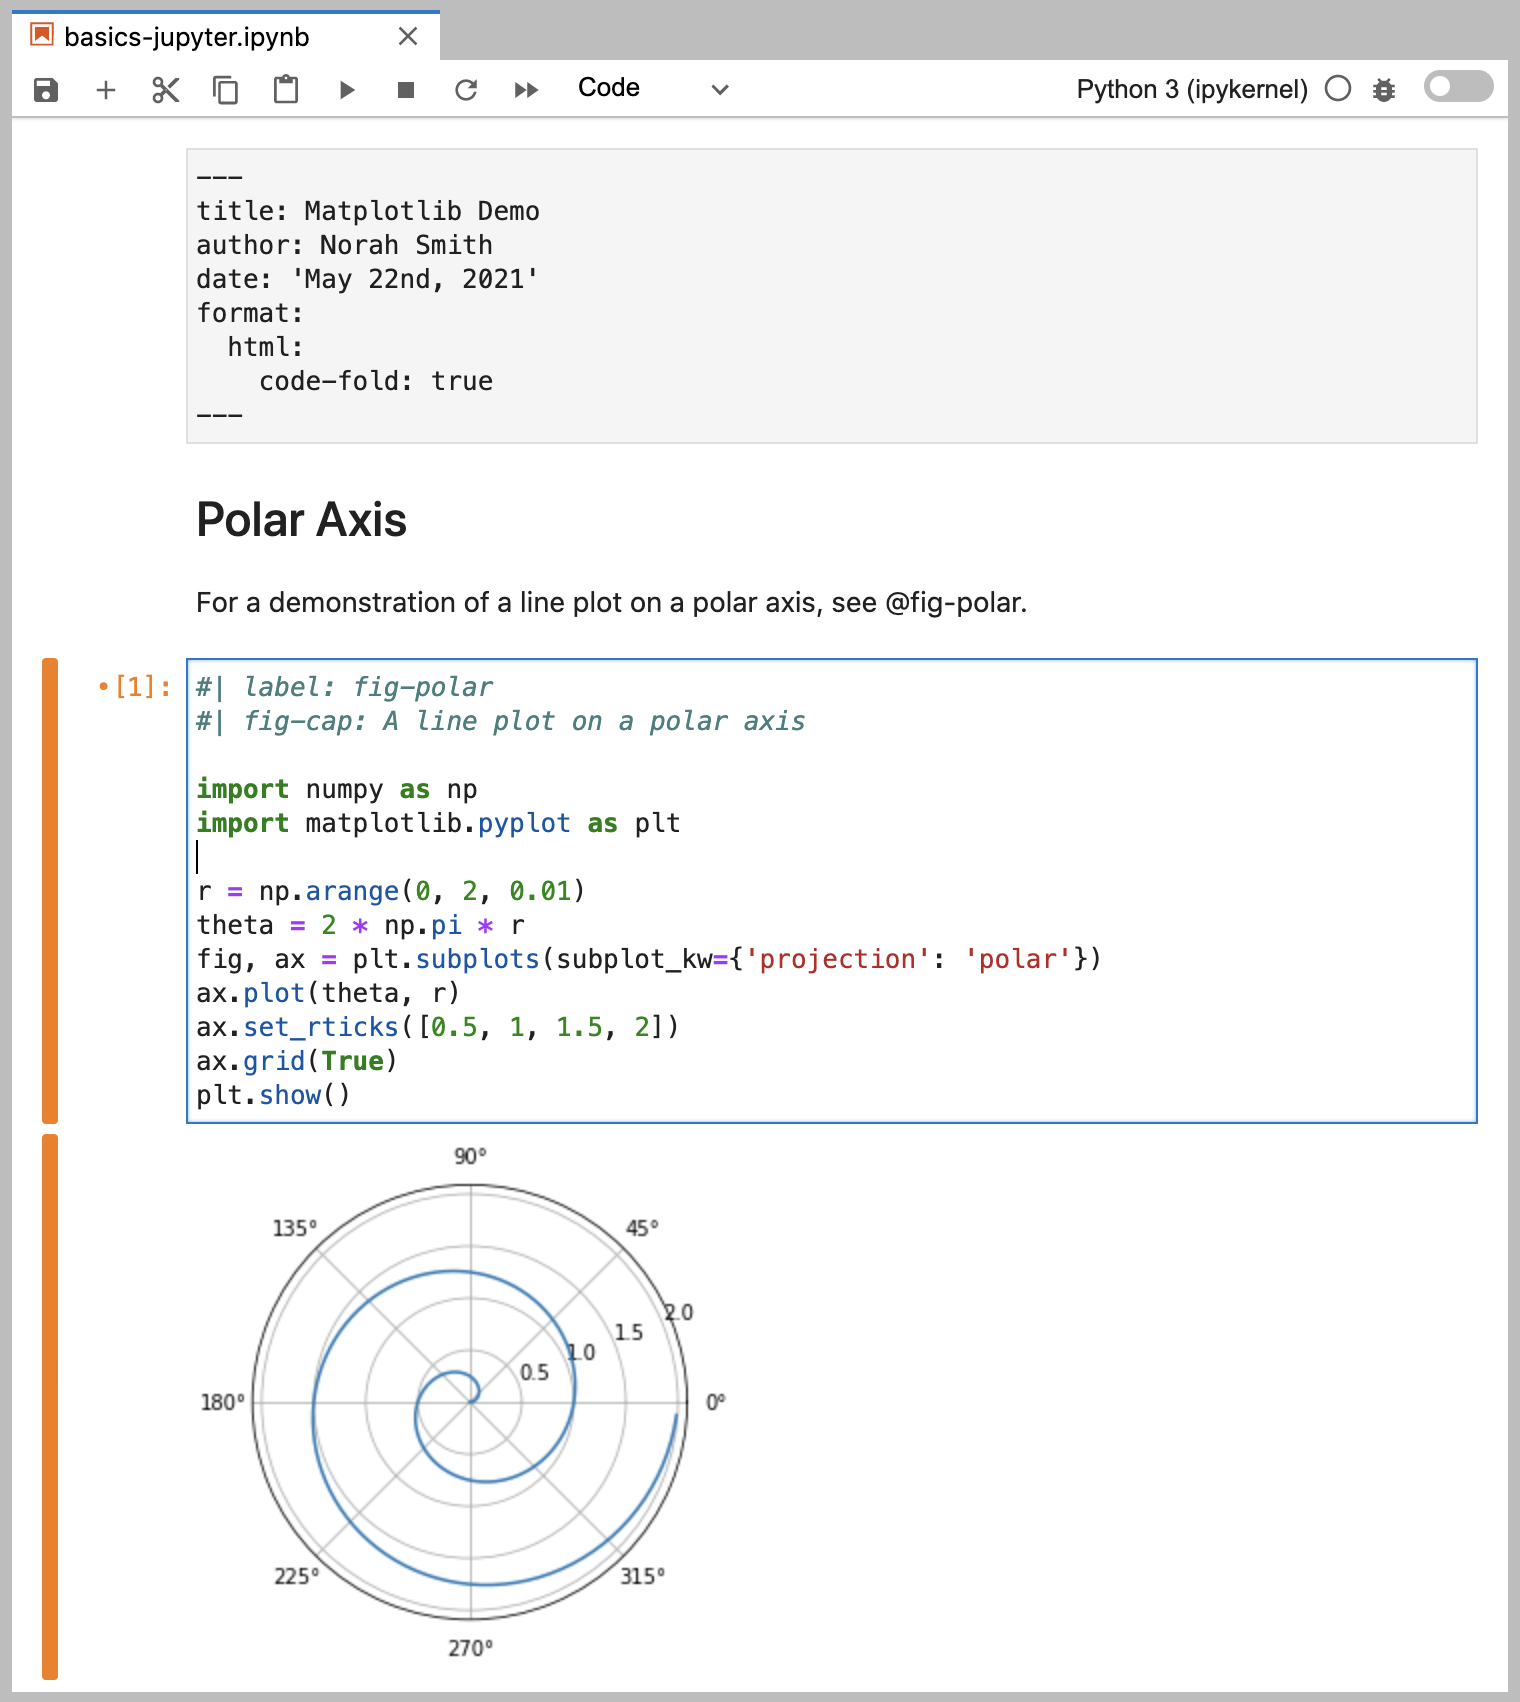
\includegraphics[keepaspectratio]{img/jupyter-lab.png}}

If you look at the source code you'll note that YAML options were
provided both at the top of the document and within the code cell. We'll
describe working with YAML options in more detail below.

\section{Workflow}\label{workflow}

The ideal workflow for authoring Quarto notebooks in JupyterLab is to
run the \texttt{quarto\ preview} command from within a terminal:

\begin{codelisting}

\caption{\texttt{Terminal}}

\begin{Shaded}
\begin{Highlighting}[]
\ExtensionTok{quarto}\NormalTok{ preview notebook.ipynb}
\end{Highlighting}
\end{Shaded}

\end{codelisting}

The notebook will be rendered and a web browser with a ``live preview''
opened. Position this browser so that you can see it as you edit and
save the notebook:

\pandocbounded{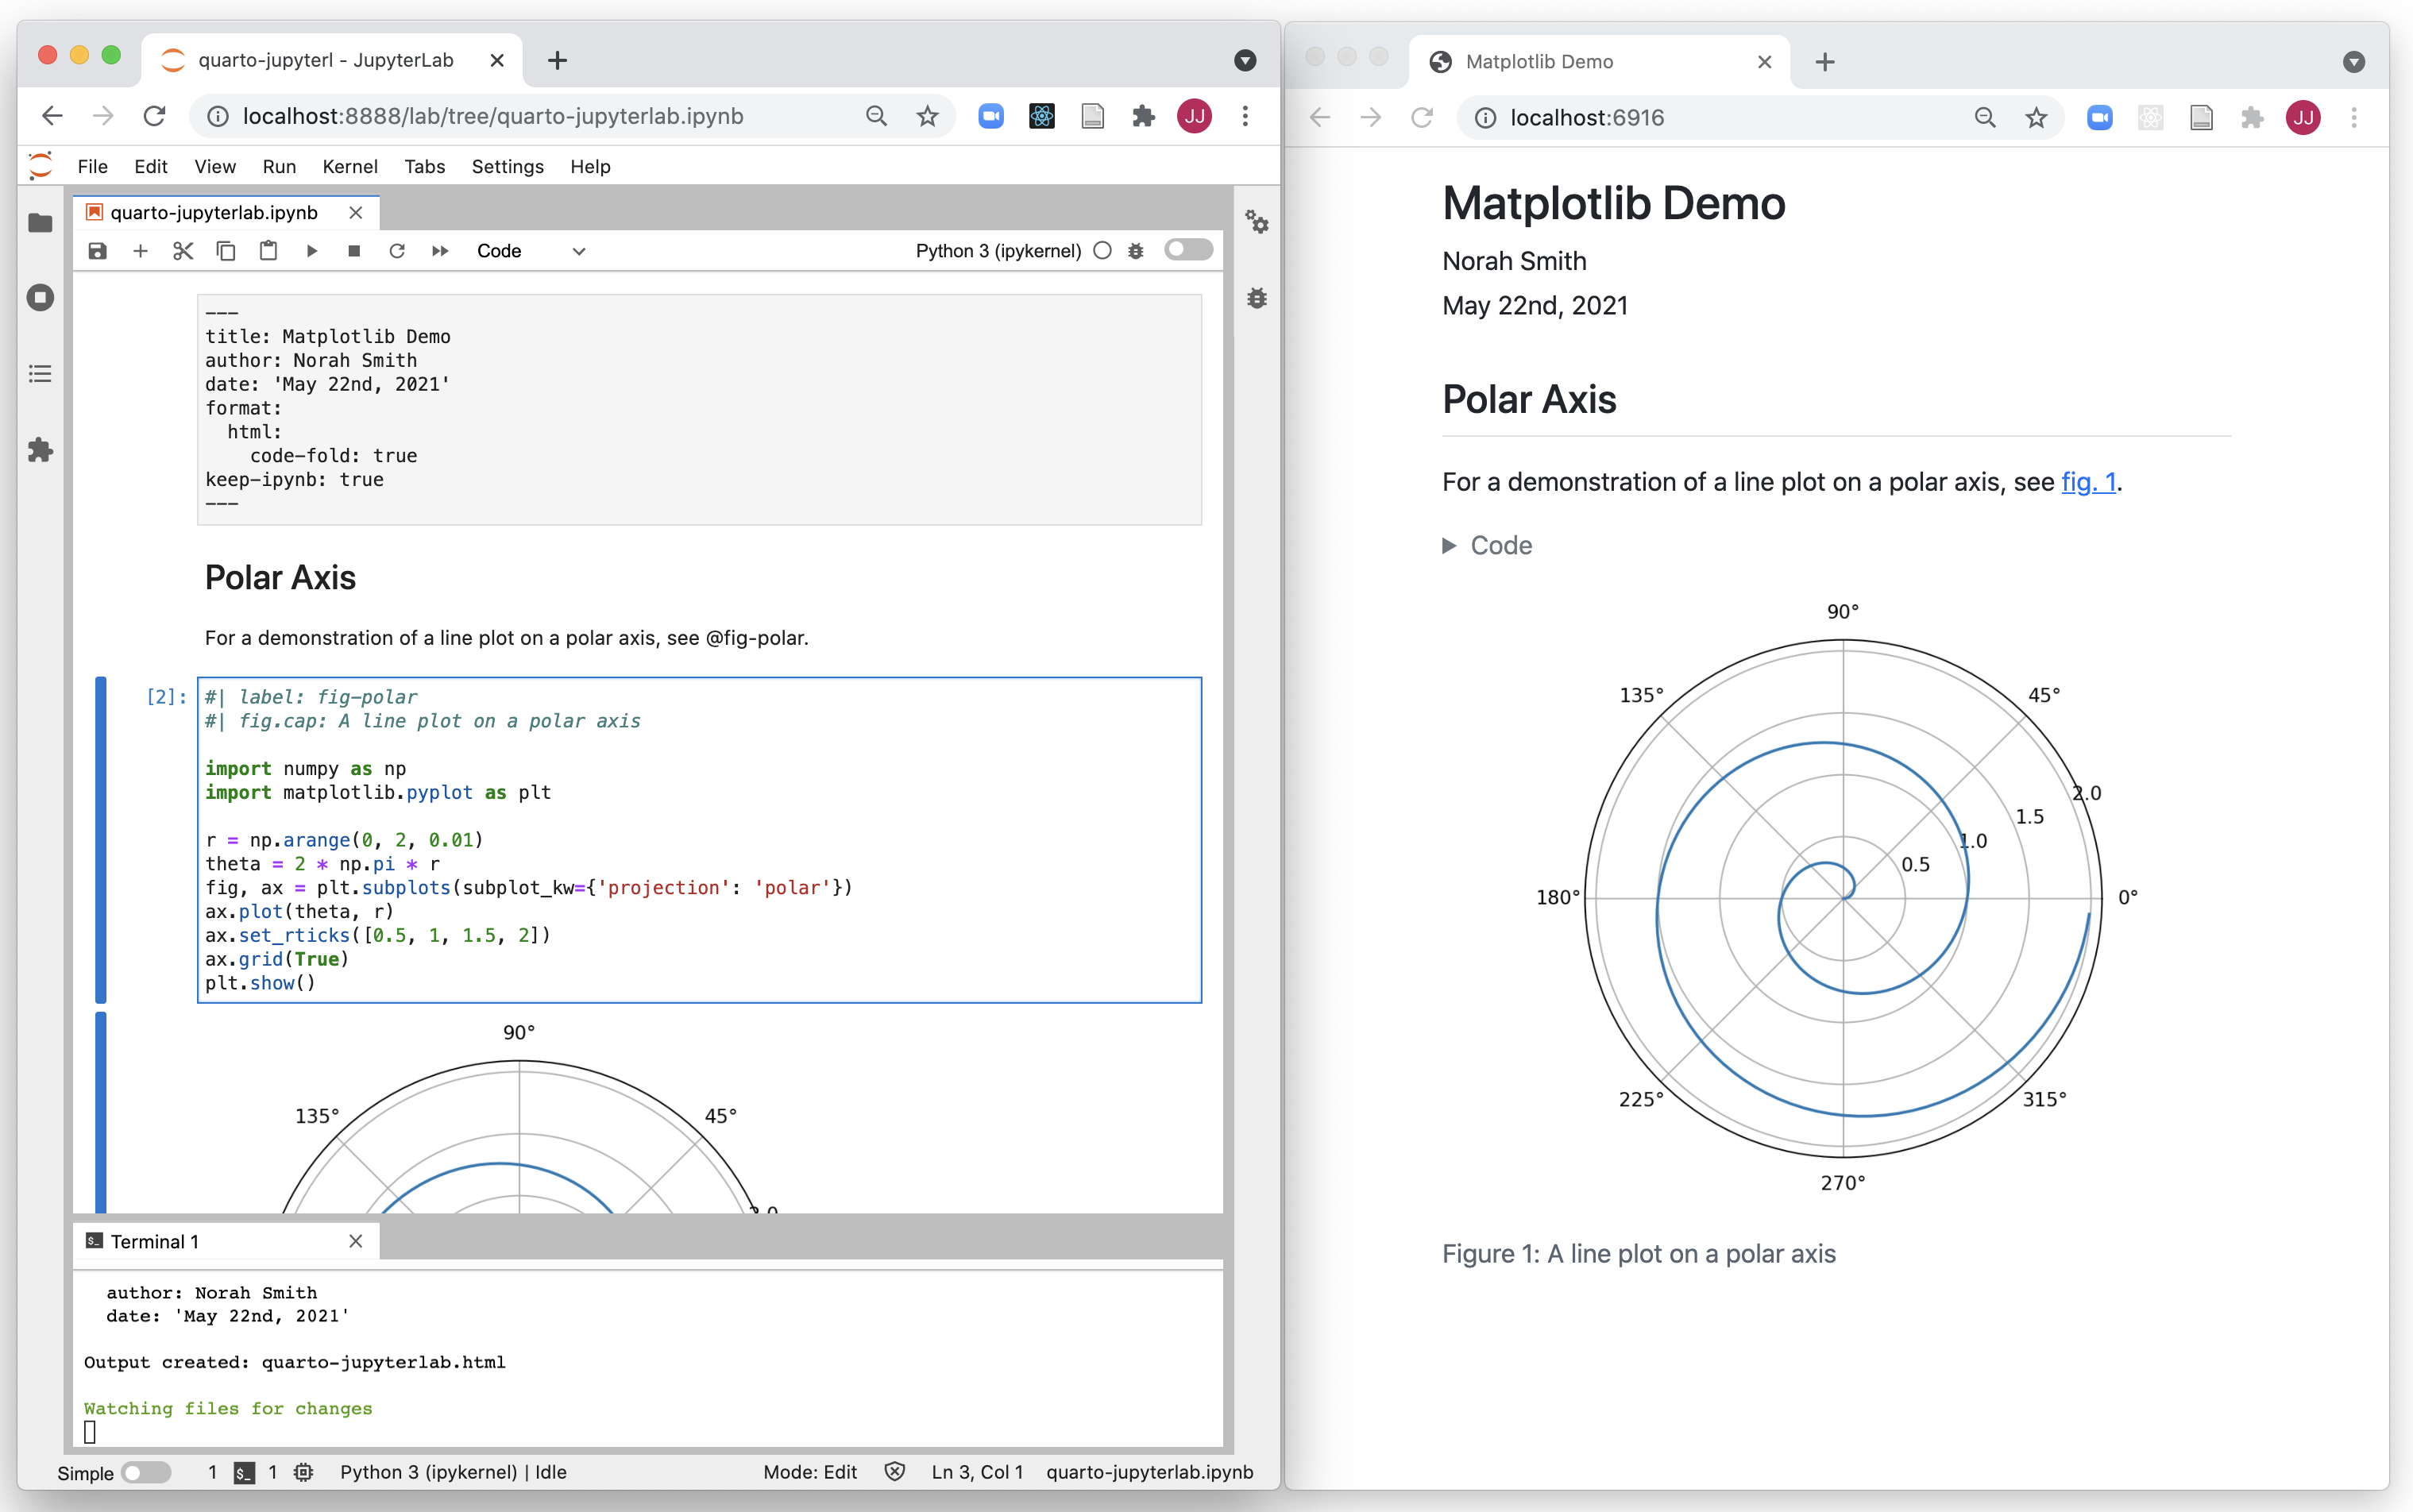
\includegraphics[keepaspectratio]{img/jupyterlab-preview.png}}

Every time you save within JupyterLab the preview will be automatically
updated. You can use \texttt{quarto\ preview} for both HTML and PDF
output.

In the screenshot above you'll note that we ran \texttt{quarto\ preview}
inside a JupyterLab terminal window---this is generally recommended so
that you can see progress and error messages when renders occur.

Preview uses the default format specified within the document---to use
an alternate format pass the \texttt{-\/-to} option to
\texttt{quarto\ preview}. For example:

\begin{codelisting}

\caption{\texttt{Terminal}}

\begin{Shaded}
\begin{Highlighting}[]
\ExtensionTok{quarto}\NormalTok{ preview notebook.ipynb }\AttributeTok{{-}{-}to}\NormalTok{ pdf}
\end{Highlighting}
\end{Shaded}

\end{codelisting}

\begin{tcolorbox}[enhanced jigsaw, arc=.35mm, bottomrule=.15mm, breakable, colback=white, colframe=quarto-callout-note-color-frame, left=2mm, leftrule=.75mm, opacityback=0, rightrule=.15mm, toprule=.15mm]
\begin{minipage}[t]{5.5mm}
\textcolor{quarto-callout-note-color}{\faInfo}
\end{minipage}%
\begin{minipage}[t]{\textwidth - 5.5mm}

Note that if you are authoring a book or website you can also use
\href{./docs/websites/website-basics.qmd\#workflow}{\texttt{quarto\ preview}}
on the project directory, which will create a live preview for the
entire project.

\end{minipage}%
\end{tcolorbox}

\subsubsection{Running JupyterLab}\label{running-jupyterlab}

To run JupyterLab, invoke the \texttt{jupyter} module from within the
shell where you are using Quarto:

{\def\LTcaptype{none} % do not increment counter
\begin{longtable}[]{@{}
  >{\raggedright\arraybackslash}p{(\linewidth - 2\tabcolsep) * \real{0.2083}}
  >{\raggedright\arraybackslash}p{(\linewidth - 2\tabcolsep) * \real{0.5417}}@{}}
\toprule\noalign{}
\begin{minipage}[b]{\linewidth}\raggedright
Platform
\end{minipage} & \begin{minipage}[b]{\linewidth}\raggedright
Command
\end{minipage} \\
\midrule\noalign{}
\endhead
\bottomrule\noalign{}
\endlastfoot
Mac/Linux & \begin{minipage}[t]{\linewidth}\raggedright
\begin{codelisting}

\caption{\texttt{Terminal}}

\begin{Shaded}
\begin{Highlighting}[]
\ExtensionTok{python3} \AttributeTok{{-}m}\NormalTok{ jupyter lab}
\end{Highlighting}
\end{Shaded}

\end{codelisting}
\end{minipage} \\
Windows & \begin{minipage}[t]{\linewidth}\raggedright
\begin{codelisting}

\caption{\texttt{Terminal}}

\begin{Shaded}
\begin{Highlighting}[]
\NormalTok{py }\OperatorTok{{-}}\NormalTok{m jupyter lab}
\end{Highlighting}
\end{Shaded}

\end{codelisting}
\end{minipage} \\
\end{longtable}
}

\subsubsection{Render without Preview}\label{render-without-preview}

You can render a notebook (or group of notebooks) without previewing
them using the \texttt{quarto\ render} command:

\begin{codelisting}

\caption{\texttt{Terminal}}

\begin{Shaded}
\begin{Highlighting}[]
\ExtensionTok{quarto}\NormalTok{ render notebook.ipynb}
\end{Highlighting}
\end{Shaded}

\end{codelisting}

Use the \texttt{-\/-to} argument to render to a specific format:

\begin{codelisting}

\caption{\texttt{Terminal}}

\begin{Shaded}
\begin{Highlighting}[]
\ExtensionTok{quarto}\NormalTok{ render notebook.ipynb }\AttributeTok{{-}{-}to}\NormalTok{ docx}
\end{Highlighting}
\end{Shaded}

\end{codelisting}

Note that the target file (in this case \texttt{notebook.ipynb}) should
always be the very first command line argument.

\subsubsection{JupyterLab Extension}\label{jupyterlab-extension}

The Quarto JuptyerLab extension enables JupyterLab Notebooks which use
Quarto markdown to properly display the contents of the markdown cells.
For example, when the Quarto JupyterLab extension is installed, your
Notebook will show rendered previews of elements like Callouts, Divs,
Mermaid charts, as well as other Quarto elements (including the document
front matter as a title block).

You can read more about installing the extension in the
\href{./docs/tools/jupyter-lab-extension.qmd}{Quarto JupyterLab
Extension} documentation.

\section{YAML Front Matter}\label{yaml-front-matter}

The first cell of your notebook should be a \textbf{Raw} cell that
contains the document title, author, and any other options you need to
specify. Note that you can switch the type of a cell to \textbf{Raw}
using the notebook toolbar:

\pandocbounded{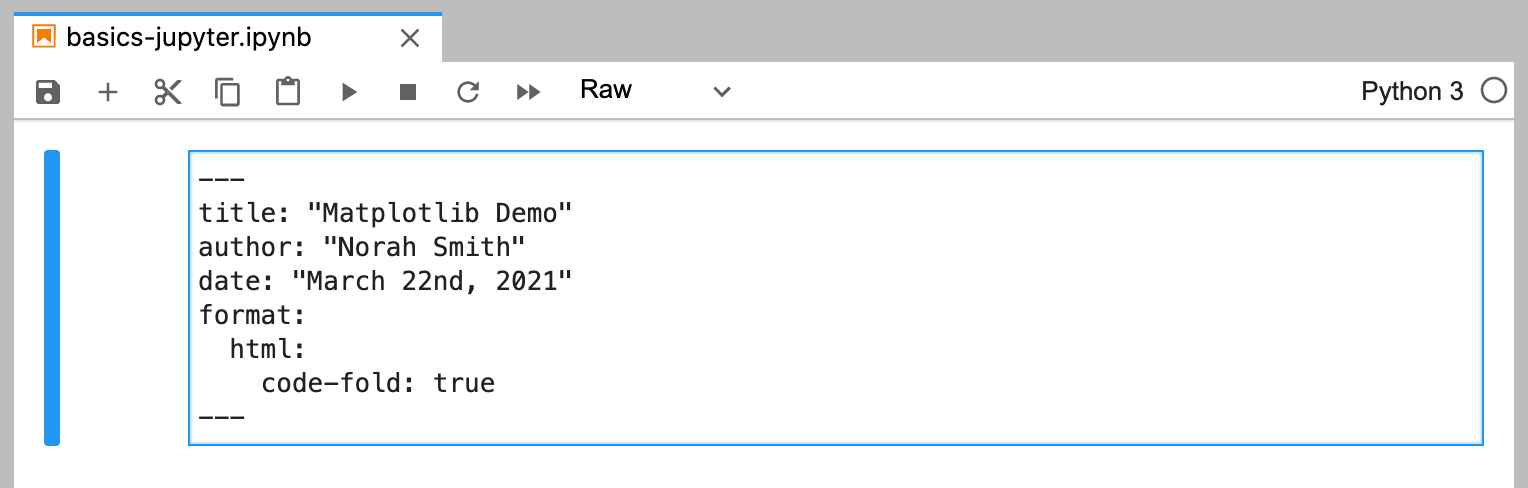
\includegraphics[keepaspectratio]{img/jupyter-lab-yaml.png}}

In this example we specify that we want code to appear collapsed by
default. There are YAML options to control many other aspects of
document rendering. See the documentation on
\href{./docs/authoring/markdown-basics.qmd}{Authoring} and
\href{./docs/output-formats/html-basics.qmd}{Output Formats} for
additional details.

\section{Markdown Cells}\label{markdown-cells}

Here's the underlying code for the markdown cell:

\pandocbounded{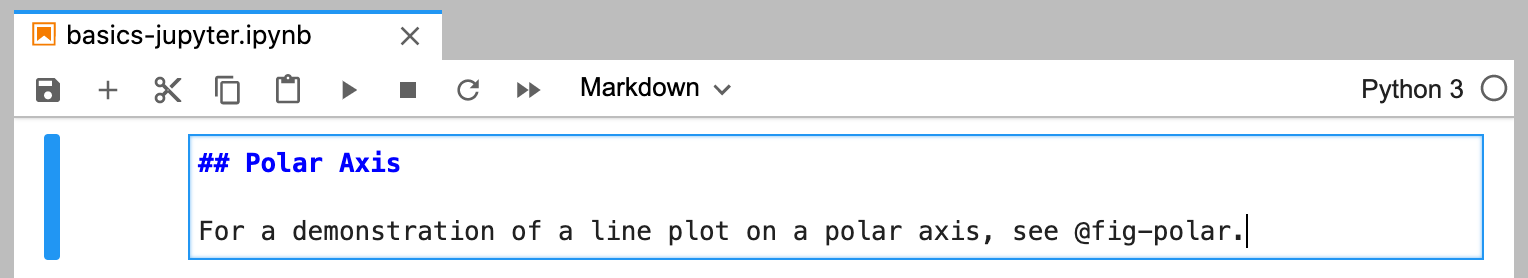
\includegraphics[keepaspectratio]{img/jupyter-lab-markdown.png}}

Note that a Quarto cross-reference (\texttt{@fig-polar}) is included in
the markdown. Any valid Pandoc markdown syntax can be included in
markdown cells.

\section{Output Options}\label{output-options}

Quarto uses leading comments with a special prefix
(\texttt{\#\textbar{}}) to denote cell options. Here we specify the
\texttt{label} and \texttt{fig-cap} options so that the plot generated
from the cell can be cross-referenced.

\pandocbounded{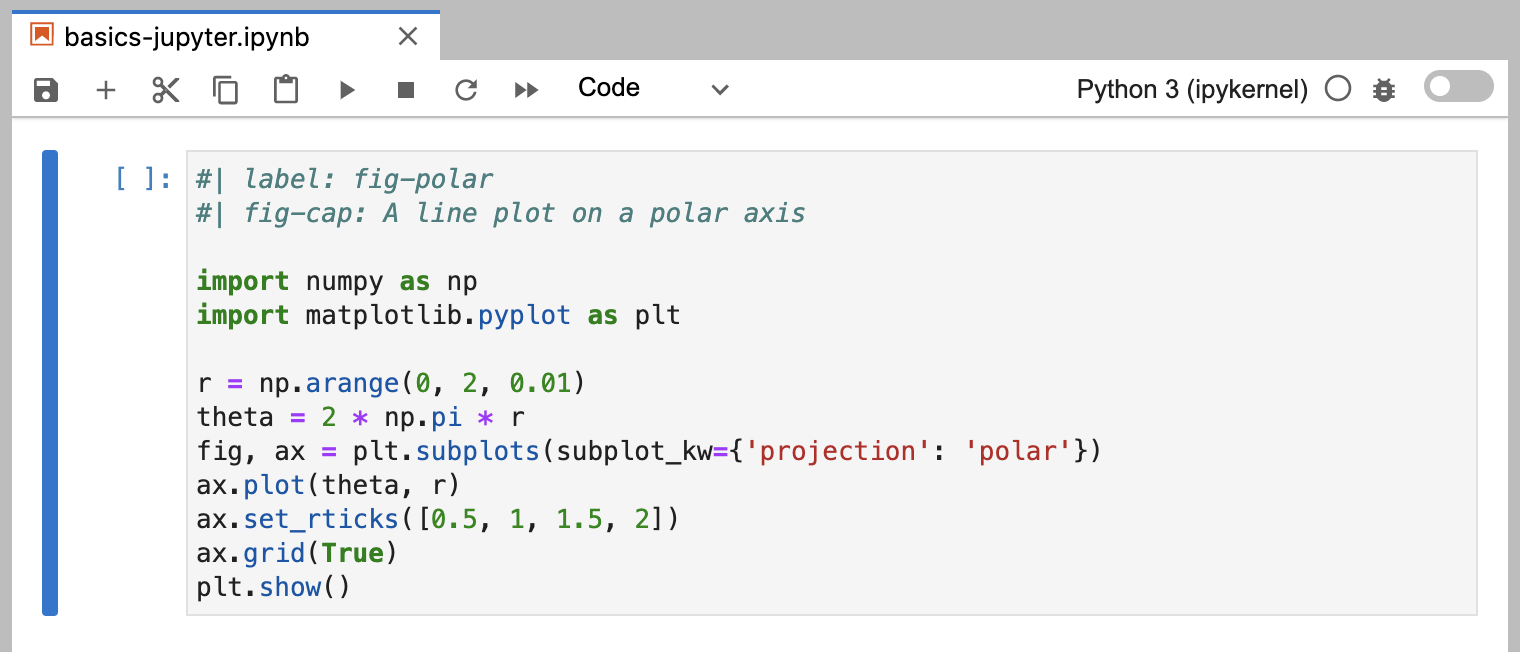
\includegraphics[keepaspectratio]{img/jupyter-lab-output-options.png}}

Note that options must appear at the very beginning of the cell. As with
document front-matter, option names/values use YAML syntax.

There are many output options available, including options to optionally
hide code, warnings, and/or output. See the documentation on
\href{./docs/computations/execution-options.qmd\#output-options}{Output
Options} for additional details.

\section{Cell Execution}\label{cell-execution}

Note that when rendering an \texttt{.ipynb} Quarto \textbf{will not}
execute the cells within the notebook by default (the presumption being
that you have already executed them while editing the notebook). If you
want to execute the cells you can pass the \texttt{-\/-execute} flag to
render:

\begin{codelisting}

\caption{\texttt{Terminal}}

\begin{Shaded}
\begin{Highlighting}[]
\ExtensionTok{quarto}\NormalTok{ render notebook.ipynb }\AttributeTok{{-}{-}execute}
\end{Highlighting}
\end{Shaded}

\end{codelisting}

You can also specify this behavior within the notebook's YAML front
matter:

\begin{codelisting}

\caption{\texttt{notebook.ipynb}}

\begin{Shaded}
\begin{Highlighting}[]
\PreprocessorTok{{-}{-}{-}}
\FunctionTok{title}\KeywordTok{:}\AttributeTok{ }\StringTok{"My Notebook"}
\FunctionTok{execute}\KeywordTok{:}\AttributeTok{ }
\AttributeTok{  }\FunctionTok{enabled}\KeywordTok{:}\AttributeTok{ }\CharTok{true}
\PreprocessorTok{{-}{-}{-}}
\end{Highlighting}
\end{Shaded}

\end{codelisting}

There are many other execution options available (e.g.~to control
caching, optimizing kernel start-up time, etc.). Learn more about these
options in \href{./docs/computations/execution-options.qmd}{Execution
Options}.

\section{Plain Text Editing}\label{plain-text-editing}

It's also possible to edit Jupyter notebooks in a plain-text markdown
format. You might prefer this if there is more narrative than code in
your notebook or if you want to use a file format that is more version
control friendly.

Here is the plain text markdown version of the notebook used in the
previous examples:

\begin{Shaded}
\begin{Highlighting}[]
\CommentTok{{-}{-}{-}}
\AnnotationTok{title:}\CommentTok{ "Matplotlib Demo"}
\AnnotationTok{author:}\CommentTok{ "Norah Smith"}
\AnnotationTok{date:}\CommentTok{ "5/22/2021"}
\AnnotationTok{format:}\CommentTok{ }
\CommentTok{  html:}
\CommentTok{    code{-}fold: true}
\AnnotationTok{jupyter:}\CommentTok{ python3}
\CommentTok{{-}{-}{-}}

\FunctionTok{\#\# Polar Axis}

\NormalTok{For a demonstration of a line plot on a polar axis, see @fig{-}polar.}

\InformationTok{\textasciigrave{}\textasciigrave{}\textasciigrave{}\{python\}}
\CommentTok{\#| label: fig{-}polar}
\CommentTok{\#| fig{-}cap: "A line plot on a polar axis"}

\ImportTok{import}\NormalTok{ numpy }\ImportTok{as}\NormalTok{ np}
\ImportTok{import}\NormalTok{ matplotlib.pyplot }\ImportTok{as}\NormalTok{ plt}

\NormalTok{r }\OperatorTok{=}\NormalTok{ np.arange(}\DecValTok{0}\NormalTok{, }\DecValTok{2}\NormalTok{, }\FloatTok{0.01}\NormalTok{)}
\NormalTok{theta }\OperatorTok{=} \DecValTok{2} \OperatorTok{*}\NormalTok{ np.pi }\OperatorTok{*}\NormalTok{ r}
\NormalTok{fig, ax }\OperatorTok{=}\NormalTok{ plt.subplots(subplot\_kw}\OperatorTok{=}\NormalTok{\{}\StringTok{\textquotesingle{}projection\textquotesingle{}}\NormalTok{: }\StringTok{\textquotesingle{}polar\textquotesingle{}}\NormalTok{\})}
\NormalTok{ax.plot(theta, r)}
\NormalTok{ax.set\_rticks([}\FloatTok{0.5}\NormalTok{, }\DecValTok{1}\NormalTok{, }\FloatTok{1.5}\NormalTok{, }\DecValTok{2}\NormalTok{])}
\NormalTok{ax.grid(}\VariableTok{True}\NormalTok{)}
\NormalTok{plt.show()}
\InformationTok{\textasciigrave{}\textasciigrave{}\textasciigrave{}}
\end{Highlighting}
\end{Shaded}

Note that we've added the \texttt{jupyter:\ python3} option to the YAML
front matter to indicate which Jupyter kernel to render with. You would
render this document with:

\begin{codelisting}

\caption{\texttt{Terminal}}

\begin{Shaded}
\begin{Highlighting}[]
\ExtensionTok{quarto}\NormalTok{ render basics{-}jupyter.qmd}
\end{Highlighting}
\end{Shaded}

\end{codelisting}

Markdown files with embedded code chunks should use the file extension
\texttt{.qmd}.

\begin{tcolorbox}[enhanced jigsaw, arc=.35mm, bottomrule=.15mm, bottomtitle=1mm, breakable, colback=white, colbacktitle=quarto-callout-tip-color!10!white, colframe=quarto-callout-tip-color-frame, coltitle=black, left=2mm, leftrule=.75mm, opacityback=0, opacitybacktitle=0.6, rightrule=.15mm, title=\textcolor{quarto-callout-tip-color}{\faLightbulb}\hspace{0.5em}{Tip}, titlerule=0mm, toprule=.15mm, toptitle=1mm]

If you are doing most of your work in .qmd files you should consider
using RStudio, which includes full support for editing .qmd files that
use Python and Jupyter (including code completion, cell-at-a-time
execution, and side-by-side preview). See the article on using
\href{rstudio.qmd}{RStudio} for additional details.

\end{tcolorbox}

\subsubsection{Converting Notebooks}\label{converting-notebooks}

You can convert between .ipynb and .qmd representations of a notebook
using the \texttt{quarto\ convert} command. For example:

\begin{codelisting}

\caption{\texttt{Terminal}}

\begin{Shaded}
\begin{Highlighting}[]
\ExtensionTok{quarto}\NormalTok{ convert basics{-}jupyter.ipynb }\CommentTok{\# converts to qmd}
\ExtensionTok{quarto}\NormalTok{ convert basics{-}jupyter.qmd   }\CommentTok{\# converts to ipynb}
\end{Highlighting}
\end{Shaded}

\end{codelisting}

See \texttt{quarto\ convert\ help} for additional details on converting
notebooks.

\subsubsection{Jupytext}\label{jupytext}

You can use Jupytext to maintain parallel synchronized versions of
\texttt{.qmd} and \texttt{.ipynb} files. Learn more about Jupytext at
\url{https://jupytext.readthedocs.io/en/latest/}.

\section{Polar Axis}\label{polar-axis}

For a demonstration of a line plot on a polar axis, see
Figure~\ref{fig-polar}.

\begin{Shaded}
\begin{Highlighting}[]
\ImportTok{import}\NormalTok{ numpy }\ImportTok{as}\NormalTok{ np}
\ImportTok{import}\NormalTok{ matplotlib.pyplot }\ImportTok{as}\NormalTok{ plt}

\NormalTok{r }\OperatorTok{=}\NormalTok{ np.arange(}\DecValTok{0}\NormalTok{, }\DecValTok{2}\NormalTok{, }\FloatTok{0.01}\NormalTok{)}
\NormalTok{theta }\OperatorTok{=} \DecValTok{2} \OperatorTok{*}\NormalTok{ np.pi }\OperatorTok{*}\NormalTok{ r}
\NormalTok{fig, ax }\OperatorTok{=}\NormalTok{ plt.subplots(}
\NormalTok{  subplot\_kw }\OperatorTok{=}\NormalTok{ \{}\StringTok{\textquotesingle{}projection\textquotesingle{}}\NormalTok{: }\StringTok{\textquotesingle{}polar\textquotesingle{}}\NormalTok{\} }
\NormalTok{)}
\NormalTok{ax.plot(theta, r)}
\NormalTok{ax.set\_rticks([}\FloatTok{0.5}\NormalTok{, }\DecValTok{1}\NormalTok{, }\FloatTok{1.5}\NormalTok{, }\DecValTok{2}\NormalTok{])}
\NormalTok{ax.grid(}\VariableTok{True}\NormalTok{)}
\NormalTok{plt.show()}
\end{Highlighting}
\end{Shaded}

\begin{figure}[H]

\centering{

\pandocbounded{
\includegraphics[keepaspectratio]{Using Jupyter Notebooks_files/figure-pdf/fig-polar-output-1.png}}

}

\caption{\label{fig-polar}A line plot on a polar axis}

\end{figure}%

\chapter{More on Markdown Syntax}\label{more-on-markdown-syntax}

Adapted from
\href{https://utrechtuniversity.github.io/open-textbooks/}{Research Data
Management Support (Utrecht University)}

\begin{quote}
Markdown is a lightweight markup language that you can use to add
formatting elements to plaintext text documents. -
\href{https://www.markdownguide.org/getting-started/}{Markdown Guide}
\end{quote}

Quarto documents contain content that is formatted with markdown. Where
in text editors, you press buttons to make text \textbf{bold},
\href{https://www.markdownguide.org/basic-syntax/\#links}{create a
hyperlink}, or create headers, in markdown you explicitly write these
elements out in the raw text. This raw markdown can then be converted to
other formats, such as HTML, pdf, epub or even Word. In a Quarto book,
this is done automatically when you \emph{render} the book.

\href{https://quarto.org/docs/authoring/markdown-basics.html}{See the
full Quarto markdown documentation}

\begin{tcolorbox}[enhanced jigsaw, arc=.35mm, bottomrule=.15mm, bottomtitle=1mm, breakable, colback=white, colbacktitle=quarto-callout-tip-color!10!white, colframe=quarto-callout-tip-color-frame, coltitle=black, left=2mm, leftrule=.75mm, opacityback=0, opacitybacktitle=0.6, rightrule=.15mm, title=\textcolor{quarto-callout-tip-color}{\faLightbulb}\hspace{0.5em}{Tip}, titlerule=0mm, toprule=.15mm, toptitle=1mm]

Some useful resources:

\begin{itemize}
\tightlist
\item
  Learn markdown interactively with the
  \href{https://www.markdowntutorial.com/}{Markdown tutorial}.
\item
  For a longer list of markdown syntax, please refer to the
  \href{https://www.markdownguide.org/cheat-sheet/}{Markdown Guide
  Cheatsheet} and
  \href{https://github.com/lifeparticle/Markdown-Cheatsheet}{this GitHub
  repository with more extensive markdown options}.
\end{itemize}

\end{tcolorbox}

\section{Basic syntax}\label{basic-syntax}

{\def\LTcaptype{none} % do not increment counter
\begin{longtable}[]{@{}
  >{\raggedright\arraybackslash}p{(\linewidth - 2\tabcolsep) * \real{0.5000}}
  >{\raggedright\arraybackslash}p{(\linewidth - 2\tabcolsep) * \real{0.4444}}@{}}
\toprule\noalign{}
\begin{minipage}[b]{\linewidth}\raggedright
Markdown Syntax
\end{minipage} & \begin{minipage}[b]{\linewidth}\raggedright
Output
\end{minipage} \\
\midrule\noalign{}
\endhead
\bottomrule\noalign{}
\endlastfoot
\begin{minipage}[t]{\linewidth}\raggedright
\begin{verbatim}
*italics* and **bold**
\end{verbatim}
\end{minipage} & \emph{italics} and \textbf{bold} \\
\begin{minipage}[t]{\linewidth}\raggedright
\begin{verbatim}
superscript^2^ / subscript~2~
\end{verbatim}
\end{minipage} & superscript\textsuperscript{2} /
subscript\textsubscript{2} \\
\begin{minipage}[t]{\linewidth}\raggedright
\begin{verbatim}
~~strikethrough~~
\end{verbatim}
\end{minipage} & \st{strikethrough} \\
\begin{minipage}[t]{\linewidth}\raggedright
\begin{verbatim}
`verbatim code`
\end{verbatim}
\end{minipage} & \texttt{verbatim\ code} \\
\begin{minipage}[t]{\linewidth}\raggedright
\begin{verbatim}
# Header 1
\end{verbatim}
\end{minipage} & \begin{minipage}[t]{\linewidth}\raggedright
\chapter*{Header 1}\label{header-1}
\addcontentsline{toc}{chapter}{Header 1}

\markboth{Header 1}{Header 1}
\end{minipage} \\
\begin{minipage}[t]{\linewidth}\raggedright
\begin{verbatim}
## Header 2
\end{verbatim}
\end{minipage} & \begin{minipage}[t]{\linewidth}\raggedright
\section*{Header 2}\label{header-2}
\addcontentsline{toc}{section}{Header 2}

\markright{Header 2}
\end{minipage} \\
\begin{minipage}[t]{\linewidth}\raggedright
\begin{verbatim}
### Header 3
\end{verbatim}
\end{minipage} & \begin{minipage}[t]{\linewidth}\raggedright
\subsection*{Header 3}\label{header-3}
\addcontentsline{toc}{subsection}{Header 3}
\end{minipage} \\
\end{longtable}
}

\section{Lists}\label{lists}

\begin{Shaded}
\begin{Highlighting}[]
\SpecialStringTok{* }\NormalTok{unordered list}
\SpecialStringTok{  + }\NormalTok{sub{-}item 1}
\SpecialStringTok{    {-} }\NormalTok{sub{-}sub{-}item 1}
\SpecialStringTok{  + }\NormalTok{sub{-}item 2}
\end{Highlighting}
\end{Shaded}

\begin{itemize}
\tightlist
\item
  unordered list

  \begin{itemize}
  \tightlist
  \item
    sub-item 1

    \begin{itemize}
    \tightlist
    \item
      sub-sub-item 1
    \end{itemize}
  \item
    sub-item 2
  \end{itemize}
\end{itemize}

\begin{Shaded}
\begin{Highlighting}[]
\SpecialStringTok{1. }\NormalTok{ordered list}
\SpecialStringTok{2. }\NormalTok{item 2}
\NormalTok{   i. sub{-}item 1}
\NormalTok{      A.  sub{-}sub{-}item 1}
\end{Highlighting}
\end{Shaded}

\begin{enumerate}
\def\labelenumi{\arabic{enumi}.}
\tightlist
\item
  ordered list
\item
  item 2

  \begin{enumerate}
  \def\labelenumii{\roman{enumii}.}
  \tightlist
  \item
    sub-item 1

    \begin{enumerate}
    \def\labelenumiii{\Alph{enumiii}.}
    \tightlist
    \item
      sub-sub-item 1
    \end{enumerate}
  \end{enumerate}
\end{enumerate}

\begin{Shaded}
\begin{Highlighting}[]
\SpecialStringTok{*   }\NormalTok{item 2}
    
\NormalTok{    Continued (indent 4 spaces)}
\end{Highlighting}
\end{Shaded}

\begin{itemize}
\item
  item 2

  Continued (indent 4 spaces)
\end{itemize}

\begin{Shaded}
\begin{Highlighting}[]
\NormalTok{term}
\NormalTok{: definition}
\end{Highlighting}
\end{Shaded}

\begin{description}
\tightlist
\item[term]
definition
\end{description}

\section{Links}\label{links}

\begin{Shaded}
\begin{Highlighting}[]
\CommentTok{[}\OtherTok{named hyperlink}\CommentTok{](https://quarto.org/)}
\end{Highlighting}
\end{Shaded}

\href{https://quarto.org/}{named hyperlink}

\begin{Shaded}
\begin{Highlighting}[]
\AnnotationTok{Direct url:}\CommentTok{ \textless{}https://quarto.org/\textgreater{}}
\end{Highlighting}
\end{Shaded}

Direct url: \url{https://quarto.org/}

\begin{Shaded}
\begin{Highlighting}[]
\NormalTok{Link to }\CommentTok{[}\OtherTok{other places}\CommentTok{](\#lists)} 
\NormalTok{in the document.}
\end{Highlighting}
\end{Shaded}

Link to \hyperref[lists]{other places} in the document.

\begin{Shaded}
\begin{Highlighting}[]
\AnnotationTok{Embed an image:}\CommentTok{ }
\AlertTok{![penguins](https://allisonhorst.github.io/palmerpenguins/reference/figures/lter\_penguins.png)}
\end{Highlighting}
\end{Shaded}

Embed an image:
\pandocbounded{\includegraphics[keepaspectratio,alt={penguins}]{index_files/mediabag/lter_penguins.png}}

\section{Tables}\label{tables}

\begin{Shaded}
\begin{Highlighting}[]
\InformationTok{    | Right | Left | Default | Center |}
\InformationTok{    |{-}{-}{-}{-}{-}{-}:|:{-}{-}{-}{-}{-}|{-}{-}{-}{-}{-}{-}{-}{-}{-}|:{-}{-}{-}{-}{-}{-}:|}
\InformationTok{    |   12  |  12  |    12   |    12  |}
\InformationTok{    |  123  |  123 |   123   |   123  |}
\InformationTok{    |    1  |    1 |     1   |     1  |}
\end{Highlighting}
\end{Shaded}

{\def\LTcaptype{none} % do not increment counter
\begin{longtable}[]{@{}rllc@{}}
\toprule\noalign{}
Right & Left & Default & Center \\
\midrule\noalign{}
\endhead
\bottomrule\noalign{}
\endlastfoot
12 & 12 & 12 & 12 \\
123 & 123 & 123 & 123 \\
1 & 1 & 1 & 1 \\
\end{longtable}
}

\begin{tcolorbox}[enhanced jigsaw, arc=.35mm, bottomrule=.15mm, bottomtitle=1mm, breakable, colback=white, colbacktitle=quarto-callout-note-color!10!white, colframe=quarto-callout-note-color-frame, coltitle=black, left=2mm, leftrule=.75mm, opacityback=0, opacitybacktitle=0.6, rightrule=.15mm, title=\textcolor{quarto-callout-note-color}{\faInfo}\hspace{0.5em}{Note}, titlerule=0mm, toprule=.15mm, toptitle=1mm]

It is possible to use raw html elements in a quarto document. But try to
limit this because:

\begin{itemize}
\tightlist
\item
  Not everyone knows how html works, so it's less accessible for others
  to work with your content.
\item
  Raw html elements will only correctly be displayed in html output. If
  you have pdf output, for example, the html elements are not rendered
  correctly.
\end{itemize}

\end{tcolorbox}

\chapter{Even more on Markdown}\label{even-more-on-markdown}

\chapter{Even more on Markdown}\label{sec-authoring}

When we say ``authoring'' we mean the process of adding content to a
Quarto document---literally, the things you write in a \texttt{.qmd}
file. More specifically, this chapter focuses on what you put in the
parts of your document that are interpreted as markdown---that is,
everything that isn't the document header, or an executable code cell.

Our goal is to give you a good overview of breadth of Quarto's authoring
features, while delaying many of the details to later chapters of the
book. We also focus on syntax that is broadly supported across multiple
output formats and cover specific format features where relevant in
\textbf{?@sec-html}, \textbf{?@sec-typst} and
\textbf{?@sec-presentations}.

We suggest reading through the chapter in its entirety on your first
reading, and then referring back to specific sections as needed when
authoring your own documents.

\section{Markdown text}\label{markdown-text}

Everything that isn't the document header or an executable code cell is
interpreted as Quarto markdown. Quarto markdown inherits much of
Pandoc's markdown syntax, but uses its own parser. This means you can
use familiar markdown syntax, though there are some differences from
Pandoc. The rest of this chapter outlines the most useful Quarto
markdown syntax.

While we distinguish between executable code cells and markdown in the
source document, this distinction disappears after rendering. When cells
execute, their output becomes markdown and is treated identically to
other markdown content. Executable code cells produce block-level
markdown, so you can only use them where block elements are allowed. For
example, as list items, inside fenced divs, or inside table cells. You
cannot use code cells inline with text or inside section headings.

\section{Sections}\label{sections}

Use markdown headings to structure your document into sections and
subsections. Markdown headings are created by prefixing text with one or
more \texttt{\#} characters, followed by a space, and the heading title:

\begin{Shaded}
\begin{Highlighting}[]
\FunctionTok{\#\# Section}

\FunctionTok{\#\#\# Subsection}

\FunctionTok{\#\#\#\# Subsubsection}
\end{Highlighting}
\end{Shaded}

Quarto supports six levels of headings, from level-1 (\texttt{\#}) to
level-6 (\texttt{\#\#\#\#\#\#}). The value of \texttt{title} in the
document header usually becomes the level-1 heading of the document,
which is why sections usually start with level-2 headings.

You can attach attributes to headings by adding curly braces
\texttt{\{\}} after the heading text. For example, you might add an
identifier to a section heading to enable cross-referencing:

\begin{Shaded}
\begin{Highlighting}[]
\FunctionTok{\#\# Section Title \{\#sec{-}section{-}title\}}
\end{Highlighting}
\end{Shaded}

Or you might add a class like \texttt{.unlisted} to exclude a section
from the table of contents:

\begin{Shaded}
\begin{Highlighting}[]
\FunctionTok{\#\# Section Title \{\#sec{-}section{-}title .unlisted\}}
\end{Highlighting}
\end{Shaded}

\begin{tcolorbox}[enhanced jigsaw, arc=.35mm, bottomrule=.15mm, bottomtitle=1mm, breakable, colback=white, colbacktitle=quarto-callout-tip-color!10!white, colframe=quarto-callout-tip-color-frame, coltitle=black, left=2mm, leftrule=.75mm, opacityback=0, opacitybacktitle=0.6, rightrule=.15mm, title=\textcolor{quarto-callout-tip-color}{\faLightbulb}\hspace{0.5em}{Tip \ref*{tip-attributes}: What are attributes?}, titlerule=0mm, toprule=.15mm, toptitle=1mm]

\quartocallouttip{tip-attributes} 

Attributes are a way to add metadata to markdown elements, usually
inside curly braces \texttt{\{\}} after the element. Attributes are used
extensively in Quarto to control the behavior or appearance of many
elements.

The types of thing you can add as attributes include:

\begin{itemize}
\tightlist
\item
  Identifiers (IDs), should be unique and start with \texttt{\#}
\item
  Classes start with \texttt{.}
\item
  Key-value pairs use
  \texttt{key=\textquotesingle{}value\textquotesingle{}} syntax.
\end{itemize}

The order of attributes matters: identifiers must come first, followed
by classes, and then key-value pairs.

\end{tcolorbox}

\section{Paragraphs}\label{paragraphs}

Create paragraphs by separating text with blank lines:

\begin{Shaded}
\begin{Highlighting}[]
\NormalTok{This is the first paragraph. It can span multiple lines }
\NormalTok{in your source document.}

\NormalTok{This is a second paragraph, separated by a blank line.}
\end{Highlighting}
\end{Shaded}

Quarto ignores line breaks within a paragraph, which means you can wrap
your text across multiple lines without affecting the final rendered
output.

\section{Text}\label{text}

Beyond plain text, Table~\ref{tbl-inline-text-elements} summarizes the
most common things you want to put inside a paragraph or heading:
formatted text, links, cross-references, citations, math and footnotes.

These elements are called \textbf{inline text elements}, because they
are used inline with text, inside what are called \textbf{block
elements} like paragraphs and headings. You can also use them inside
many of the other block-level elements discussed in this chapter like as
list items, inside tables, and inside callouts.

\begin{longtable}[]{@{}
  >{\raggedright\arraybackslash}p{(\linewidth - 4\tabcolsep) * \real{0.2500}}
  >{\raggedright\arraybackslash}p{(\linewidth - 4\tabcolsep) * \real{0.5000}}
  >{\raggedright\arraybackslash}p{(\linewidth - 4\tabcolsep) * \real{0.2500}}@{}}
\caption[]{Common syntax for inline text elements in Quarto markdown.
TODO: Element column entries will span
rows.}\label{tbl-inline-text-elements}\tabularnewline
\toprule\noalign{}
\begin{minipage}[b]{\linewidth}\raggedright
Element
\end{minipage} & \begin{minipage}[b]{\linewidth}\raggedright
Output
\end{minipage} & \begin{minipage}[b]{\linewidth}\raggedright
Markdown Syntax
\end{minipage} \\
\midrule\noalign{}
\endfirsthead
\toprule\noalign{}
\begin{minipage}[b]{\linewidth}\raggedright
Element
\end{minipage} & \begin{minipage}[b]{\linewidth}\raggedright
Output
\end{minipage} & \begin{minipage}[b]{\linewidth}\raggedright
Markdown Syntax
\end{minipage} \\
\midrule\noalign{}
\endhead
\bottomrule\noalign{}
\endlastfoot
\multirow{7}{=}{ \textbf{Text formatting}} & \emph{italics},
\textbf{bold}, \textbf{\emph{bold italics}} &
\begin{minipage}[t]{\linewidth}\raggedright
\begin{Shaded}
\begin{Highlighting}[]
\NormalTok{*italics*, **bold**, ***bold italics***}
\end{Highlighting}
\end{Shaded}
\end{minipage} \\
& superscript\textsuperscript{2} / subscript\textsubscript{2} &
\begin{minipage}[t]{\linewidth}\raggedright
\begin{Shaded}
\begin{Highlighting}[]
\NormalTok{superscript\^{}2\^{} / subscript\textasciitilde{}2\textasciitilde{}}
\end{Highlighting}
\end{Shaded}
\end{minipage} \\
& \st{strikethrough} & \begin{minipage}[t]{\linewidth}\raggedright
\begin{Shaded}
\begin{Highlighting}[]
\NormalTok{\textasciitilde{}\textasciitilde{}strikethrough\textasciitilde{}\textasciitilde{}}
\end{Highlighting}
\end{Shaded}
\end{minipage} \\
& \texttt{verbatim\ code} & \begin{minipage}[t]{\linewidth}\raggedright
\begin{Shaded}
\begin{Highlighting}[]
\InformationTok{\textasciigrave{}verbatim code\textasciigrave{}}
\end{Highlighting}
\end{Shaded}
\end{minipage} \\
& \textsc{smallcaps} & \begin{minipage}[t]{\linewidth}\raggedright
\begin{Shaded}
\begin{Highlighting}[]
\CommentTok{[}\OtherTok{smallcaps}\CommentTok{]}\NormalTok{\{.smallcaps\}}
\end{Highlighting}
\end{Shaded}
\end{minipage} \\
& \ul{underlined} & \begin{minipage}[t]{\linewidth}\raggedright
\begin{Shaded}
\begin{Highlighting}[]
\CommentTok{[}\OtherTok{underlined}\CommentTok{]}\NormalTok{\{.underline\}}
\end{Highlighting}
\end{Shaded}
\end{minipage} \\
& \hl{highlighted} & \begin{minipage}[t]{\linewidth}\raggedright
\begin{Shaded}
\begin{Highlighting}[]
\CommentTok{[}\OtherTok{highlighted}\CommentTok{]}\NormalTok{\{.mark\}}
\end{Highlighting}
\end{Shaded}
\end{minipage} \\
\multirow{3}{=}{ \textbf{Links}} & \url{https://quarto.org} &
\begin{minipage}[t]{\linewidth}\raggedright
\begin{Shaded}
\begin{Highlighting}[]
\OtherTok{\textless{}https://quarto.org\textgreater{}}
\end{Highlighting}
\end{Shaded}
\end{minipage} \\
& \href{https://quarto.org}{Quarto} &
\begin{minipage}[t]{\linewidth}\raggedright
\begin{Shaded}
\begin{Highlighting}[]
\CommentTok{[}\OtherTok{Quarto}\CommentTok{](https://quarto.org)}
\end{Highlighting}
\end{Shaded}
\end{minipage} \\
& \hyperref[links]{Links section} &
\begin{minipage}[t]{\linewidth}\raggedright
\begin{Shaded}
\begin{Highlighting}[]
\CommentTok{[}\OtherTok{Links section}\CommentTok{](\#links)}
\end{Highlighting}
\end{Shaded}
\end{minipage} \\
\textbf{Math} Section~\ref{sec-equations} & Inline math: \(E = mc^{2}\)
& \begin{minipage}[t]{\linewidth}\raggedright
\begin{Shaded}
\begin{Highlighting}[]
\AnnotationTok{Inline math:}\CommentTok{ $E = mc\^{}\{2\}$}
\end{Highlighting}
\end{Shaded}
\end{minipage} \\
\multirow{2}{=}{ \textbf{Cross-references} See
Section~\ref{sec-crossreferences}} & Figure~\ref{fig-elephant} &
\begin{minipage}[t]{\linewidth}\raggedright
\begin{Shaded}
\begin{Highlighting}[]
\NormalTok{@fig{-}elephant}
\end{Highlighting}
\end{Shaded}
\end{minipage} \\
& Chapter~\ref{sec-authoring} &
\begin{minipage}[t]{\linewidth}\raggedright
\begin{Shaded}
\begin{Highlighting}[]
\NormalTok{@sec{-}authoring}
\end{Highlighting}
\end{Shaded}
\end{minipage} \\
\multirow{3}{=}{ \textbf{Citations} Section~\ref{sec-citations}} & Knuth
(1984) shows \ldots{} & \begin{minipage}[t]{\linewidth}\raggedright
\begin{Shaded}
\begin{Highlighting}[]
\NormalTok{@knuth84 shows ...}
\end{Highlighting}
\end{Shaded}
\end{minipage} \\
& \ldots{} (Knuth 1984) & \begin{minipage}[t]{\linewidth}\raggedright
\begin{Shaded}
\begin{Highlighting}[]
\NormalTok{... }\CommentTok{[}\OtherTok{@knuth84}\CommentTok{]}
\end{Highlighting}
\end{Shaded}
\end{minipage} \\
& (Knuth 1984; Wickham et al. 2023) &
\begin{minipage}[t]{\linewidth}\raggedright
\begin{Shaded}
\begin{Highlighting}[]
\CommentTok{[}\OtherTok{@knuth84; @wickham2023}\CommentTok{]}
\end{Highlighting}
\end{Shaded}
\end{minipage} \\
\textbf{Footnotes} Section~\ref{sec-footnotes} & An inline
note.\footnote{Content} & \begin{minipage}[t]{\linewidth}\raggedright
\begin{Shaded}
\begin{Highlighting}[]
\NormalTok{An inline note.\^{}}\CommentTok{[}\OtherTok{Content}\CommentTok{]}
\end{Highlighting}
\end{Shaded}
\end{minipage} \\
\end{longtable}

\section{Lists}\label{lists-1}

You can create an unordered list by starting each line with \texttt{-}
(or \texttt{*} or \texttt{+}) followed by a space, ensuring there is a
blank line before the first element:

\begin{Shaded}
\begin{Highlighting}[]
\AnnotationTok{My list:}

\SpecialStringTok{{-} }\NormalTok{First item}
\SpecialStringTok{{-} }\NormalTok{Second item}
\SpecialStringTok{{-} }\NormalTok{Third item}
\end{Highlighting}
\end{Shaded}

Leaving no blank lines between items will result in a compact list,
while leaving a blank line between items will create a loose list with
more vertical spacing.

Use numbers followed by a period to create an ordered list:

\begin{Shaded}
\begin{Highlighting}[]
\AnnotationTok{My numbered list:}

\SpecialStringTok{1. }\NormalTok{First item}
\SpecialStringTok{2. }\NormalTok{Second item}
\SpecialStringTok{3. }\NormalTok{Third item}
\end{Highlighting}
\end{Shaded}

The actual numbers you use doesn't matter---Quarto will renumber the
list automatically. You could use \texttt{1.} for every item if you
prefer.

List items can contain other block elements like paragraphs, code
blocks, or even other lists. Subsequent elements should be indented to
line up with the first non-space content after the list marker.
Figure~\ref{fig-nested-list} shows an example of a nested list, along
with its rendered output.

\begin{figure}

\centering{

\begin{Shaded}
\begin{Highlighting}[]
\SpecialStringTok{{-} }\NormalTok{First item with multiple paragraphs.}

\NormalTok{  This is the second paragraph, }
\NormalTok{  indented to align with the first paragraph.}

\SpecialStringTok{{-} }\NormalTok{An item with a sublist:}

\SpecialStringTok{  1. }\NormalTok{Subitem one}
\SpecialStringTok{  2. }\NormalTok{Subitem two}

\SpecialStringTok{{-} }\NormalTok{Third item}

  \InformationTok{\textasciigrave{}\textasciigrave{}\textasciigrave{}\{.python\}}
  \CommentTok{\# This is a code block inside a list item}
  \InformationTok{\textasciigrave{}\textasciigrave{}\textasciigrave{}}
\end{Highlighting}
\end{Shaded}

\begin{itemize}
\item
  First item with multiple paragraphs.

  This is the second paragraph, indented to align with the first
  paragraph.
\item
  An item with a sublist:

  \begin{enumerate}
  \def\labelenumi{\arabic{enumi}.}
  \tightlist
  \item
    Subitem one
  \item
    Subitem two
  \end{enumerate}
\item
  Third item

\begin{Shaded}
\begin{Highlighting}[]
\CommentTok{\# This is a code block inside a list item}
\end{Highlighting}
\end{Shaded}
\end{itemize}

}

\caption{\label{fig-nested-list}List syntax and its rendered output}

\end{figure}%

Quarto also supports task lists and definition lists. See the
\href{https://quarto.org/docs/authoring/markdown-basics.html\#lists}{Quarto
documentation} for details on these specialized list types.

\section{Code blocks}\label{sec-code-blocks}

We use the term \textbf{code blocks}, as distinct from \textbf{code
cells}, for code that is to be shown, but never executed.

There are two equivalent syntaxes for code blocks. You can use triple
backticks followed by the language name:

\begin{Shaded}
\begin{Highlighting}[]
\InformationTok{\textasciigrave{}\textasciigrave{}\textasciigrave{}sql}
\KeywordTok{SELECT} \OperatorTok{*} \KeywordTok{FROM} \KeywordTok{table}\NormalTok{;}
\InformationTok{\textasciigrave{}\textasciigrave{}\textasciigrave{}}
\end{Highlighting}
\end{Shaded}

Or use triple backticks followed by curly braces with the language name
prefaced by a period:

\begin{Shaded}
\begin{Highlighting}[]
\InformationTok{\textasciigrave{}\textasciigrave{}\textasciigrave{}\{.sql\}}
\KeywordTok{SELECT} \OperatorTok{*} \KeywordTok{FROM} \KeywordTok{table}\NormalTok{;}
\InformationTok{\textasciigrave{}\textasciigrave{}\textasciigrave{}}
\end{Highlighting}
\end{Shaded}

We prefer the second syntax since it's easier to add additional code
block attributes. For example, you might add \texttt{filename} which
adds a header with the filename above the code block as shown in
Figure~\ref{fig-code-block-with-filename}.

\begin{figure}

\centering{

\begin{Shaded}
\begin{Highlighting}[]
\InformationTok{\textasciigrave{}\textasciigrave{}\textasciigrave{}\{.sql filename="query.sql"\}}
\KeywordTok{SELECT} \OperatorTok{*} \KeywordTok{FROM} \KeywordTok{table}\NormalTok{;}
\InformationTok{\textasciigrave{}\textasciigrave{}\textasciigrave{}}
\end{Highlighting}
\end{Shaded}

\begin{codelisting}

\caption{\texttt{query.sql}}

\begin{Shaded}
\begin{Highlighting}[]
\KeywordTok{SELECT} \OperatorTok{*} \KeywordTok{FROM} \KeywordTok{table}\NormalTok{;}
\end{Highlighting}
\end{Shaded}

\end{codelisting}

}

\caption{\label{fig-code-block-with-filename}Code block syntax and its
rendered output}

\end{figure}%

\begin{tcolorbox}[enhanced jigsaw, arc=.35mm, bottomrule=.15mm, bottomtitle=1mm, breakable, colback=white, colbacktitle=quarto-callout-tip-color!10!white, colframe=quarto-callout-tip-color-frame, coltitle=black, left=2mm, leftrule=.75mm, opacityback=0, opacitybacktitle=0.6, rightrule=.15mm, title=\textcolor{quarto-callout-tip-color}{\faLightbulb}\hspace{0.5em}{Supported code block languages}, titlerule=0mm, toprule=.15mm, toptitle=1mm]

The language for code blocks is used only for syntax highlighting. You
can see a list of supported languages by running the following command
in your terminal:

\begin{codelisting}[H]

\caption{\texttt{Terminal}}

\begin{Shaded}
\begin{Highlighting}[]
\ExtensionTok{quarto}\NormalTok{ pandoc }\AttributeTok{{-}{-}list{-}highlight{-}style} 
\end{Highlighting}
\end{Shaded}

\end{codelisting}

Specifying a language that isn't supported will simply result in no
syntax highlighting being applied.

\end{tcolorbox}

\section{Tables}\label{sec-markdown-tables}

The simplest way to add a table to a Quarto document is to create a
\textbf{markdown pipe table}, however cells in a markdown pipe table
cannot contain block content like multiple paragraphs, code cells, or
lists. To have cells with complicated cell contents, you can use an
alternative syntax called \textbf{list tables}. You can also use
\textbf{HTML table syntax}, regardless of your target format, to create
tables in Quarto documents. You won't usually write HTML syntax by hand,
but it is a common output from computational packages that create
tables.

Tables are so important in Quarto documents that we dedicate an entire
part of this book to them. For more details, see \textbf{?@sec-figtab}.

\subsection{Markdown pipe tables}\label{markdown-pipe-tables}

The simplest syntax for a table in Quarto markdown is known as the
\textbf{pipe table}, named because columns are separated by the pipe
(\texttt{\textbar{}}) character. A pipe table consists of column
headers, a separator row of dashes (\texttt{-}) and pipes
(\texttt{\textbar{}}), and data rows with pipe-separated cells.

Figure~\ref{fig-markdown-table} gives an example of a pipe table, along
with its rendered output. The line after the table, starting with
\texttt{:}, is optional, and specifies the caption and any attributes
for the table (inside curly braces \texttt{\{\}}). For example, the
table is given the ID \texttt{\#tbl-perf} so it is numbered and can be
cross-referenced.

\begin{figure}

\centering{

\begin{Shaded}
\begin{Highlighting}[]
\PreprocessorTok{|}\NormalTok{ Algorithm           }\PreprocessorTok{|}\NormalTok{ Accuracy }\PreprocessorTok{|}\NormalTok{ Time  }\PreprocessorTok{|}
\PreprocessorTok{|{-}{-}{-}{-}{-}{-}{-}{-}{-}{-}{-}{-}{-}{-}{-}{-}{-}{-}{-}{-}{-}|{-}{-}{-}{-}{-}{-}{-}{-}{-}{-}|{-}{-}{-}{-}{-}{-}{-}|}
\PreprocessorTok{|}\NormalTok{ Random Forest       }\PreprocessorTok{|}\NormalTok{ 96.7\%    }\PreprocessorTok{|}\NormalTok{ 0.12s }\PreprocessorTok{|}
\PreprocessorTok{|}\NormalTok{ Logistic Regression }\PreprocessorTok{|}\NormalTok{ 81.2\%    }\PreprocessorTok{|}\NormalTok{ 0.08s }\PreprocessorTok{|}
\PreprocessorTok{|}\NormalTok{ Linear Regression   }\PreprocessorTok{|}\NormalTok{ 74.8\%    }\PreprocessorTok{|}\NormalTok{ 0.05s }\PreprocessorTok{|}

\NormalTok{: Training performance \{\#tbl{-}perf\}}
\end{Highlighting}
\end{Shaded}

\pandocbounded{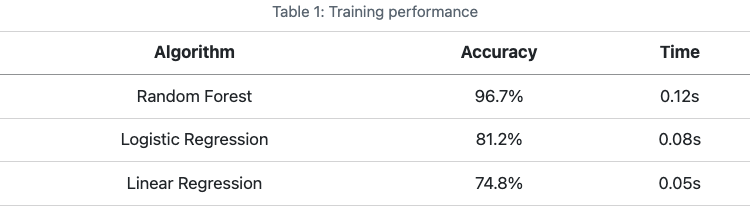
\includegraphics[keepaspectratio]{img/authoring-tbl-perf.png}}

}

\caption{\label{fig-markdown-table}Markdown syntax and rendered output
for a markdown pipe table}

\end{figure}%

\subsection{List tables}\label{list-tables}

TODO: Revisit this once the \texttt{list-tables} extension is bundled
with Quarto. Specifically, where does the caption go.

List tables use markdown list syntax to create tables where cells can
contain multiple paragraphs, code cells, or lists. List tables need to
be wrapped in a fenced div with the class \texttt{list-table}. Inside
the div, each row is represented as list item, with each cell as an
subitem.

For example, to create the same table content as
Figure~\ref{fig-markdown-table} using a list table, you would include
the following in your document:

\begin{Shaded}
\begin{Highlighting}[]
\NormalTok{::: \{\#tbl{-}perf .list{-}table\}}
\NormalTok{Training performance }

\SpecialStringTok{* }\NormalTok{{-} Algorithm}
\SpecialStringTok{  {-} }\NormalTok{Accuracy}
\SpecialStringTok{  {-} }\NormalTok{Time}
\SpecialStringTok{* }\NormalTok{{-} Random Forest}
\SpecialStringTok{  {-} }\NormalTok{96.7\%}
\SpecialStringTok{  {-} }\NormalTok{0.12s}
\SpecialStringTok{* }\NormalTok{{-} Logistic Regression}
\SpecialStringTok{  {-} }\NormalTok{81.2\%}
\SpecialStringTok{  {-} }\NormalTok{0.08s}
\SpecialStringTok{* }\NormalTok{{-} Linear Regression}
\SpecialStringTok{  {-} }\NormalTok{74.8\%}
\SpecialStringTok{  {-} }\NormalTok{0.05s}
\NormalTok{:::}
\end{Highlighting}
\end{Shaded}

To include more complicated content in cells, like code blocks or
formulas, include them as you would in normal markdown, but maintain
indentation for the list structure, and the required white space for the
content type:

\begin{Shaded}
\begin{Highlighting}[]
\NormalTok{::: \{.list{-}table\}}
\SpecialStringTok{* }\NormalTok{{-} Code}
\SpecialStringTok{  {-} }\NormalTok{Model for the mean}
\SpecialStringTok{* }\NormalTok{{-} }
    
    \InformationTok{\textasciigrave{}\textasciigrave{}\textasciigrave{}r}
    \FunctionTok{summary}\NormalTok{(}\FunctionTok{lm}\NormalTok{(mpg }\SpecialCharTok{\textasciitilde{}}\NormalTok{ wt }\SpecialCharTok{+}\NormalTok{ cyl, }\AttributeTok{data =}\NormalTok{ mtcars))}
    \InformationTok{\textasciigrave{}\textasciigrave{}\textasciigrave{}}

\SpecialStringTok{  {-} }
\NormalTok{    $$}
\NormalTok{    \textbackslash{}beta\_0 + \textbackslash{}beta\_1 \textbackslash{}text\{wt\} + \textbackslash{}beta\_2 \textbackslash{}text\{cyl\}}
\NormalTok{    $$}
\NormalTok{:::}
\end{Highlighting}
\end{Shaded}

\subsection{HTML tables}\label{html-tables}

You can also use HTML to create tables in Quarto documents, regardless
of your target format. You typically won't write HTML tables by
hand---instead, you'll generate them with code cells or import them from
other tools.

As an example, to generate the same table as
Figure~\ref{fig-markdown-table} with HTML, you could include the
following in your document:

\begin{Shaded}
\begin{Highlighting}[]
\InformationTok{\textasciigrave{}\textasciigrave{}\textasciigrave{}\{=html\}}
\InformationTok{\textless{}table id="tbl{-}perf"\textgreater{}}
\InformationTok{  \textless{}caption\textgreater{}Training performance\textless{}/caption\textgreater{}}
\InformationTok{  \textless{}thead\textgreater{}}
\InformationTok{    \textless{}tr\textgreater{}}
\InformationTok{      \textless{}th\textgreater{}Algorithm\textless{}/th\textgreater{}}
\InformationTok{      \textless{}th\textgreater{}Accuracy\textless{}/th\textgreater{}}
\InformationTok{      \textless{}th\textgreater{}Time\textless{}/th\textgreater{}}
\InformationTok{    \textless{}/tr\textgreater{}}
\InformationTok{  \textless{}/thead\textgreater{}}
\InformationTok{  \textless{}tbody\textgreater{}}
\InformationTok{    \textless{}tr\textgreater{}}
\InformationTok{      \textless{}td\textgreater{}Random Forest\textless{}/td\textgreater{}}
\InformationTok{      \textless{}td\textgreater{}96.7\%\textless{}/td\textgreater{}}
\InformationTok{      \textless{}td\textgreater{}0.12s\textless{}/td\textgreater{}}
\InformationTok{    \textless{}/tr\textgreater{}}
\InformationTok{    \textless{}tr\textgreater{}}
\InformationTok{      \textless{}td\textgreater{}Logistic Regression\textless{}/td\textgreater{}}
\InformationTok{      \textless{}td\textgreater{}81.2\%\textless{}/td\textgreater{}}
\InformationTok{      \textless{}td\textgreater{}0.08s\textless{}/td\textgreater{}}
\InformationTok{    \textless{}/tr\textgreater{}}
\InformationTok{    \textless{}tr\textgreater{}}
\InformationTok{      \textless{}td\textgreater{}Linear Regression\textless{}/td\textgreater{}}
\InformationTok{      \textless{}td\textgreater{}74.8\%\textless{}/td\textgreater{}}
\InformationTok{      \textless{}td\textgreater{}0.05s\textless{}/td\textgreater{}}
\InformationTok{    \textless{}/tr\textgreater{}}
\InformationTok{  \textless{}/tbody\textgreater{}}
\InformationTok{\textless{}/table\textgreater{}}
\InformationTok{\textasciigrave{}\textasciigrave{}\textasciigrave{}}
\end{Highlighting}
\end{Shaded}

\subsection{From a code cell}\label{sec-computational-table}

When the output from an executable code cell is a markdown or HTML
table, it will be included in your Quarto document.

To add an identifier and caption to the table use the code cell options
\texttt{label} and \texttt{tbl-cap} respectively:

\begin{Shaded}
\begin{Highlighting}[]
\InformationTok{\textasciigrave{}\textasciigrave{}\textasciigrave{}\{LANGUAGE\}}
\InformationTok{\#| label: tbl{-}example}
\InformationTok{\#| tbl{-}cap: "Caption"}

\InformationTok{\# Code that generates a markdown or HTML table}
\InformationTok{\textasciigrave{}\textasciigrave{}\textasciigrave{}}
\end{Highlighting}
\end{Shaded}

\section{Images and figures}\label{sec-markdown-figures}

You can include images in your document either from an image file, or
from the output of an executable code cell.

Figures are so important in Quarto documents that we dedicate an entire
part of this book to them. For more details, see \textbf{?@sec-figtab}.

\begin{tcolorbox}[enhanced jigsaw, arc=.35mm, bottomrule=.15mm, bottomtitle=1mm, breakable, colback=white, colbacktitle=quarto-callout-tip-color!10!white, colframe=quarto-callout-tip-color-frame, coltitle=black, left=2mm, leftrule=.75mm, opacityback=0, opacitybacktitle=0.6, rightrule=.15mm, title=\textcolor{quarto-callout-tip-color}{\faLightbulb}\hspace{0.5em}{Image or figure?}, titlerule=0mm, toprule=.15mm, toptitle=1mm]

We use the term \textbf{figure} to refer to any image, numbered or not,
included in a document. You may be more used to using the term figure to
refer to an image with a numbered caption---we'll call this a
\textbf{cross-referenceable figure}.

\end{tcolorbox}

\subsection{From a file}\label{from-a-file}

To include an image file in markdown you use the following syntax:

\begin{Shaded}
\begin{Highlighting}[]
\AlertTok{![](path/to/image.png)}
\end{Highlighting}
\end{Shaded}

Where the path to the image is a path relative to the current document.

\begin{tcolorbox}[enhanced jigsaw, arc=.35mm, bottomrule=.15mm, bottomtitle=1mm, breakable, colback=white, colbacktitle=quarto-callout-tip-color!10!white, colframe=quarto-callout-tip-color-frame, coltitle=black, left=2mm, leftrule=.75mm, opacityback=0, opacitybacktitle=0.6, rightrule=.15mm, title=\textcolor{quarto-callout-tip-color}{\faLightbulb}\hspace{0.5em}{Project relative paths}, titlerule=0mm, toprule=.15mm, toptitle=1mm]

If you preface the path with \texttt{/}, it is interpreted as a path
relative to the project root. You'll learn more about project structure
in \hyperref[sec-projects]{Projects}.

\end{tcolorbox}

You can add a caption inside the square brackets, an identifier inside
curly braces after the image path, and alternative text for
accessibility in a \texttt{fig-alt} attribute:

\begin{Shaded}
\begin{Highlighting}[]
\AlertTok{![Caption](path/to/image.png)}\NormalTok{\{\#fig{-}quarto fig{-}alt="Alternative text"\}}
\end{Highlighting}
\end{Shaded}

If your identifier starts with \texttt{fig-}, the image will be a
cross-referenceable figure, numbered, and can be referenced using the
\texttt{@} syntax.

\subsection{From a code cell}\label{sec-computational-figure}

If the output from an executable code cell is an image, it will be
automatically included in your document. To add an identifier, caption,
or alternative text use the code cell options \texttt{label},
\texttt{fig-cap}, and \texttt{fig-alt} respectively:

\begin{Shaded}
\begin{Highlighting}[]
\InformationTok{\textasciigrave{}\textasciigrave{}\textasciigrave{}\{LANGUAGE\}}
\InformationTok{\#| label: fig{-}quarto}
\InformationTok{\#| fig{-}cap: "Caption"}
\InformationTok{\#| fig{-}alt: "Alternative text"}

\InformationTok{\# Code that generates a plot}
\InformationTok{\textasciigrave{}\textasciigrave{}\textasciigrave{}}
\end{Highlighting}
\end{Shaded}

\section{Mathematical equations}\label{sec-equations}

You can include formulas and equations in your document using TeX
syntax. There are two ways to include math: \textbf{inline math}, using
single \texttt{\$}, appears within a line of text; while \textbf{display
math}, using \texttt{\$\$} appears centered on its own line.
Table~\ref{tbl-math-examples} shows examples of both.

To number and cross-reference a display equation, add an identifier
starting with \texttt{eq-}, see Section~\ref{sec-crossreferences} for
more details.

\begin{longtable}[]{@{}
  >{\raggedright\arraybackslash}p{(\linewidth - 4\tabcolsep) * \real{0.2500}}
  >{\raggedright\arraybackslash}p{(\linewidth - 4\tabcolsep) * \real{0.5000}}
  >{\raggedright\arraybackslash}p{(\linewidth - 4\tabcolsep) * \real{0.2500}}@{}}
\caption[]{Math syntax examples and their rendered
output}\label{tbl-math-examples}\tabularnewline
\toprule\noalign{}
\begin{minipage}[b]{\linewidth}\raggedright
Element
\end{minipage} & \begin{minipage}[b]{\linewidth}\raggedright
Output
\end{minipage} & \begin{minipage}[b]{\linewidth}\raggedright
Markdown Syntax
\end{minipage} \\
\midrule\noalign{}
\endfirsthead
\toprule\noalign{}
\begin{minipage}[b]{\linewidth}\raggedright
Element
\end{minipage} & \begin{minipage}[b]{\linewidth}\raggedright
Output
\end{minipage} & \begin{minipage}[b]{\linewidth}\raggedright
Markdown Syntax
\end{minipage} \\
\midrule\noalign{}
\endhead
\bottomrule\noalign{}
\endlastfoot
Inline math & \ldots{} \(E = mc^{2}\) \ldots{} &
\begin{minipage}[t]{\linewidth}\raggedright
\begin{Shaded}
\begin{Highlighting}[]
\NormalTok{... $E = mc\^{}\{2\}$ ...}
\end{Highlighting}
\end{Shaded}
\end{minipage} \\
Display math & The formula is: \(
E = mc^{2}
\) & \begin{minipage}[t]{\linewidth}\raggedright
\begin{Shaded}
\begin{Highlighting}[]
\AnnotationTok{The formula is:}\CommentTok{ }
\NormalTok{$$}
\NormalTok{E = mc\^{}\{2\}}
\NormalTok{$$}
\end{Highlighting}
\end{Shaded}
\end{minipage} \\
\end{longtable}

\section{Cross-references}\label{sec-crossreferences}

Cross-references are automatically generated links to elements within
your document, like figures, tables, sections, and equations. When you
render your document, Quarto automatically numbers these elements and
creates the links.

To create a cross-reference you need to do two things:

\begin{enumerate}
\def\labelenumi{\arabic{enumi}.}
\item
  \textbf{Add an identifier} to the element you want to reference using
  an identifier that starts with a specific prefix.
\item
  \textbf{Reference the element} elsewhere in your document using
  \texttt{@} followed by the identifier.
\end{enumerate}

Table~\ref{tbl-crossref-prefixes} give examples of common elements,
their prefixes and an example of adding the identifier as an attribute.
For computational outputs, like figures and tables generated from code
cells, you add the identifier using the \texttt{label} code cell option.
You can see an example for a table in
Section~\ref{sec-computational-table}, a figure in
Section~\ref{sec-computational-figure}, and many more details in
\textbf{?@sec-figtab-crossrefs}.

\begin{longtable}[]{@{}
  >{\raggedright\arraybackslash}p{(\linewidth - 4\tabcolsep) * \real{0.2000}}
  >{\raggedright\arraybackslash}p{(\linewidth - 4\tabcolsep) * \real{0.4000}}
  >{\raggedright\arraybackslash}p{(\linewidth - 4\tabcolsep) * \real{0.4000}}@{}}
\caption[]{Common cross-reference
types}\label{tbl-crossref-prefixes}\tabularnewline
\toprule\noalign{}
\begin{minipage}[b]{\linewidth}\raggedright
Element Type
\end{minipage} & \begin{minipage}[b]{\linewidth}\raggedright
Prefix
\end{minipage} & \begin{minipage}[b]{\linewidth}\raggedright
Markdown
\end{minipage} \\
\midrule\noalign{}
\endfirsthead
\toprule\noalign{}
\begin{minipage}[b]{\linewidth}\raggedright
Element Type
\end{minipage} & \begin{minipage}[b]{\linewidth}\raggedright
Prefix
\end{minipage} & \begin{minipage}[b]{\linewidth}\raggedright
Markdown
\end{minipage} \\
\midrule\noalign{}
\endhead
\bottomrule\noalign{}
\endlastfoot
Figure & \texttt{fig-} & \begin{minipage}[t]{\linewidth}\raggedright
\begin{Shaded}
\begin{Highlighting}[]
\AlertTok{![Caption](image.png)}\NormalTok{\{\#fig{-}elephant\}}
\end{Highlighting}
\end{Shaded}
\end{minipage} \\
Table & \texttt{tbl-} & \begin{minipage}[t]{\linewidth}\raggedright
\begin{Shaded}
\begin{Highlighting}[]
\PreprocessorTok{|}\NormalTok{ Header 1 }\PreprocessorTok{|}\NormalTok{ Header 2 }\PreprocessorTok{|}
\PreprocessorTok{|{-}{-}{-}{-}{-}{-}{-}{-}{-}{-}|{-}{-}{-}{-}{-}{-}{-}{-}{-}{-}|}
\PreprocessorTok{|}\NormalTok{ Data 1   }\PreprocessorTok{|}\NormalTok{ Data 2   }\PreprocessorTok{|}

\NormalTok{: Caption \{\#tbl{-}results\}}
\end{Highlighting}
\end{Shaded}
\end{minipage} \\
Section & \texttt{sec-} & \begin{minipage}[t]{\linewidth}\raggedright
\begin{Shaded}
\begin{Highlighting}[]
\FunctionTok{\#\# Introduction \{\#sec{-}intro\}}
\end{Highlighting}
\end{Shaded}
\end{minipage} \\
Equation & \texttt{eq-} & \begin{minipage}[t]{\linewidth}\raggedright
\begin{Shaded}
\begin{Highlighting}[]
\NormalTok{$$}
\NormalTok{a\^{}2 + b\^{}2 = c\^{}2 }
\NormalTok{$$ \{\#eq{-}py\}}
\end{Highlighting}
\end{Shaded}
\end{minipage} \\
Code listing & \texttt{lst-} &
\begin{minipage}[t]{\linewidth}\raggedright
\begin{Shaded}
\begin{Highlighting}[]
\InformationTok{\textasciigrave{}\textasciigrave{}\textasciigrave{}\{\#lst{-}example .python\}}
\InformationTok{\textasciigrave{}\textasciigrave{}\textasciigrave{}}
\end{Highlighting}
\end{Shaded}
\end{minipage} \\
Theorem & \texttt{thm-}, see
\href{https://quarto.org/docs/authoring/cross-references.html\#theorems-and-proofs}{Quarto
docs} for other theorem-like environments &
\begin{minipage}[t]{\linewidth}\raggedright
\begin{Shaded}
\begin{Highlighting}[]
\NormalTok{::: \{\#thm{-}main\}}
\FunctionTok{\#\# Theorem name}

\NormalTok{Theorem content}
\NormalTok{:::}
\end{Highlighting}
\end{Shaded}
\end{minipage} \\
Callouts & \texttt{nte-}, \texttt{tip-}, \texttt{wrn-}, \texttt{imp-},
\texttt{cau-} & \begin{minipage}[t]{\linewidth}\raggedright
\begin{Shaded}
\begin{Highlighting}[]
\NormalTok{:::\{\#nte{-}df .callout{-}note\}}
\FunctionTok{\#\# Heading}

\NormalTok{Content}
\NormalTok{:::}
\end{Highlighting}
\end{Shaded}
\end{minipage} \\
\end{longtable}

Once labeled, you can cross-reference an element using the \texttt{@}
syntax. Table~\ref{tbl-crossref-examples} gives examples of this syntax.

\begin{longtable}[]{@{}lll@{}}
\caption[]{Examples of cross-reference syntax and their rendered
output}\label{tbl-crossref-examples}\tabularnewline
\toprule\noalign{}
Description & Output & Markdown syntax \\
\midrule\noalign{}
\endfirsthead
\toprule\noalign{}
Description & Output & Markdown syntax \\
\midrule\noalign{}
\endhead
\bottomrule\noalign{}
\endlastfoot
Basic reference & Figure~\ref{fig-elephant} & \texttt{@fig-elephant} \\
Custom prefix & Fig~\ref{fig-elephant} &
\texttt{{[}Fig\ @fig-elephant{]}} \\
Number only & \ref{fig-elephant} & \texttt{{[}-@fig-elephant{]}} \\
Multiple references &
Figure~\ref{fig-elephant}, Figure~\ref{fig-panther} &
\texttt{{[}@fig-elephant;\ @fig-panther{]}} \\
\end{longtable}

For more details on cross-referencing specific element types, see the
\href{https://quarto.org/docs/authoring/cross-references.html}{Quarto
documentation}.

\begin{figure}

\begin{minipage}[t]{0.50\linewidth}

\begin{figure}[H]

\centering{


\includegraphics[width=0.25\linewidth,height=\textheight,keepaspectratio]{img/elephant.png}

}

\caption{\label{fig-elephant}Elephant}

\end{figure}%

\end{minipage}%
%
\begin{minipage}[t]{0.50\linewidth}

\begin{figure}[H]

\centering{


\includegraphics[width=0.25\linewidth,height=\textheight,keepaspectratio]{img/panther.png}

}

\caption{\label{fig-panther}Panther}

\end{figure}%

\end{minipage}%
\newline
\begin{minipage}[t]{0.50\linewidth}
Some placeholder images for cross-referencing examples\end{minipage}%

\end{figure}%

\section{Citations}\label{sec-citations}

You can automatically generate citations and a bibliography in a number
of styles. To do so you need:

\begin{enumerate}
\def\labelenumi{\arabic{enumi}.}
\item
  A bibliographic data source, for example a BibLaTeX (\texttt{.bib}) or
  BibTeX (\texttt{.bibtex}) file.
\item
  A quarto document formatted with citations (see
  \hyperref[sec-citations]{Citation Markdown}).
\end{enumerate}

Add a bibliography file to your document using the \texttt{bibliography}
YAML metadata field. For example:

\begin{Shaded}
\begin{Highlighting}[]
\PreprocessorTok{{-}{-}{-}}
\FunctionTok{title}\KeywordTok{:}\AttributeTok{ }\StringTok{"My Document"}
\FunctionTok{bibliography}\KeywordTok{:}\AttributeTok{ references.bib}
\PreprocessorTok{{-}{-}{-}}
\end{Highlighting}
\end{Shaded}

See Tip~\ref{tip-bib} for an example \texttt{references.bib} file. Then
you can cite references from the bibliography file using their
identifiers and the citation syntax described in
Table~\ref{tbl-citation-syntax}.

When you render your document, Quarto will automatically generate a
bibliography at the end of your document with all cited references
(Figure~\ref{fig-references-section}).

\begin{longtable}[]{@{}
  >{\raggedright\arraybackslash}p{(\linewidth - 2\tabcolsep) * \real{0.5000}}
  >{\raggedright\arraybackslash}p{(\linewidth - 2\tabcolsep) * \real{0.5000}}@{}}
\caption[]{Common citation
syntax}\label{tbl-citation-syntax}\tabularnewline
\toprule\noalign{}
Markdown Syntax & Output \\
\midrule\noalign{}
\endfirsthead
\toprule\noalign{}
Markdown Syntax & Output \\
\midrule\noalign{}
\endhead
\bottomrule\noalign{}
\endlastfoot
\begin{Shaded}
\begin{Highlighting}[]
\NormalTok{@knuth84 shows ...}
\end{Highlighting}
\end{Shaded}
& Knuth (1984) shows \ldots{} \\
\begin{Shaded}
\begin{Highlighting}[]
\NormalTok{... }\CommentTok{[}\OtherTok{@knuth84}\CommentTok{]}
\end{Highlighting}
\end{Shaded}
& \ldots{} (Knuth 1984) \\
\begin{Shaded}
\begin{Highlighting}[]
\NormalTok{As Knuth }\CommentTok{[}\OtherTok{{-}@knuth84}\CommentTok{]}\NormalTok{ shows ...}
\end{Highlighting}
\end{Shaded}
& As Knuth (1984) shows \ldots{} \\
\begin{Shaded}
\begin{Highlighting}[]
\CommentTok{[}\OtherTok{@knuth84; @wickham2023}\CommentTok{]}
\end{Highlighting}
\end{Shaded}
& (Knuth 1984; Wickham et al. 2023) \\
\end{longtable}

\begin{figure}

\centering{

\section*{References}\label{references}

\markright{References}

\protect\phantomsection\label{refs}
\begin{CSLReferences}{1}{1}
\bibitem[\citeproctext]{ref-DeAngelisEtAl2023}
De Angelis, Emanuele, Guglielmo De Angelis, and Maurizio Proietti. 2023.
{``A Classification Study on Testing and Verification of AI-Based
Systems.''} \emph{2023 IEEE International Conference on Artificial
Intelligence Testing (AITest)}, 1--8.
\url{https://doi.org/10.1109/AITest58265.2023.00010}.

\bibitem[\citeproctext]{ref-knuth84}
Knuth, Donald E. 1984. {``Literate Programming.''} \emph{Comput. J.}
(USA) 27 (2): 97--111. \url{https://doi.org/10.1093/comjnl/27.2.97}.

\bibitem[\citeproctext]{ref-wickham2023}
Wickham, Hadley, Mine Çetinkaya-Rundel, and Garrett Grolemund. 2023.
\emph{R for Data Science: Import, Tidy, Transform, Visualize, and Model
Data}. 2nd ed. O'Reilly Media. \url{https://r4ds.hadley.nz/}.

\end{CSLReferences}

}

\caption{\label{fig-references-section}Automatically generated
references section}

\end{figure}%

The appearance of the citations both inline and in the bibliography
depends on the citation style as defined in a CSL file. By default,
Quarto uses the \href{https://chicagomanualofstyle.org/}{Chicago Manual
of Style} author-date format, but you can provide a custom CSL file
using the \texttt{csl} option field in your document header, for
example:

\begin{Shaded}
\begin{Highlighting}[]
\PreprocessorTok{{-}{-}{-}}
\FunctionTok{title}\KeywordTok{:}\AttributeTok{ }\StringTok{"My Document"}
\FunctionTok{bibliography}\KeywordTok{:}\AttributeTok{ references.bib}
\FunctionTok{csl}\KeywordTok{:}\AttributeTok{ nature.csl}
\PreprocessorTok{{-}{-}{-}}
\end{Highlighting}
\end{Shaded}

\begin{tcolorbox}[enhanced jigsaw, arc=.35mm, bottomrule=.15mm, bottomtitle=1mm, breakable, colback=white, colbacktitle=quarto-callout-tip-color!10!white, colframe=quarto-callout-tip-color-frame, coltitle=black, left=2mm, leftrule=.75mm, opacityback=0, opacitybacktitle=0.6, rightrule=.15mm, title=\textcolor{quarto-callout-tip-color}{\faLightbulb}\hspace{0.5em}{Tip \ref*{tip-bib}: What's in \texttt{references.bib}?}, titlerule=0mm, toprule=.15mm, toptitle=1mm]

\quartocallouttip{tip-bib} 

A \texttt{.bib} file is a plain text file that contains bibliographic
entries in a specific format:

\begin{codelisting}[H]

\caption{\texttt{references.bib}}

\begin{Shaded}
\begin{Highlighting}[]
\VariableTok{@article}\NormalTok{\{}\OtherTok{knuth84}\NormalTok{,}
  \DataTypeTok{author}\NormalTok{ = \{Knuth, Donald E.\},}
  \DataTypeTok{title}\NormalTok{ = \{Literate Programming\},}
  \DataTypeTok{year}\NormalTok{ = \{1984\},}
  \DataTypeTok{issue\_date}\NormalTok{ = \{May 1984\},}
  \DataTypeTok{publisher}\NormalTok{ = \{Oxford University Press, Inc.\},}
  \DataTypeTok{address}\NormalTok{ = \{USA\},}
  \DataTypeTok{volume}\NormalTok{ = \{27\},}
  \DataTypeTok{number}\NormalTok{ = \{2\},}
  \DataTypeTok{issn}\NormalTok{ = \{0010{-}4620\},}
  \DataTypeTok{url}\NormalTok{ = \{https://doi.org/10.1093/comjnl/27.2.97\},}
  \DataTypeTok{doi}\NormalTok{ = \{10.1093/comjnl/27.2.97\},}
  \DataTypeTok{journal}\NormalTok{ = \{Comput. J.\},}
  \DataTypeTok{month}\NormalTok{ = }\StringTok{may}\NormalTok{,}
  \DataTypeTok{pages}\NormalTok{ = \{97–111\},}
  \DataTypeTok{numpages}\NormalTok{ = \{15\}}
\NormalTok{\}}

\VariableTok{@InProceedings}\NormalTok{\{}\OtherTok{DeAngelisEtAl2023}\NormalTok{,}
  \DataTypeTok{author}\NormalTok{           = \{De Angelis, Emanuele and De Angelis, Guglielmo and Proietti, Maurizio\},}
  \DataTypeTok{booktitle}\NormalTok{        = \{2023 IEEE International Conference On Artificial Intelligence Testing (AITest)\},}
  \DataTypeTok{title}\NormalTok{            = \{A Classification Study on Testing and Verification of AI{-}based Systems\},}
  \DataTypeTok{year}\NormalTok{             = \{2023\},}
  \DataTypeTok{month}\NormalTok{            = \{July\},}
  \DataTypeTok{pages}\NormalTok{            = \{1{-}8\},}
  \DataTypeTok{abstract}\NormalTok{         = \{Recent advances in Artificial Intelligence (AI) have paved the way for the development of new generations of self{-}adaptive systems that embed learning behaviours. Often these systems make use of Machine Learning (ML) models and algorithms, others make use of symbolic reasoning, or a combination of the two. A problem common to all these solutions is the difficulty in establishing clear conformance criteria that can be used to reliably assess whether an AI{-}based software system (and, in particular, ML{-}based) is behaving as intended, i.e., according to its specification. Research communities from different areas are investigating innovative V\&V approaches in order to assess evolving AI systems against their expected functionalities. This empirical study identifies, collects and categorises relevant research papers on testing and formal verification of AI{-}based software systems. In total, we have considered a set of 78 fully qualified primary studies from the digital library Scopus. For each of them, we have mapped their key aspects into a classification framework that supports their comparison across a set of common dimensions.\},}
  \DataTypeTok{comment}\NormalTok{          = \{p6: Our study suggests that, among the various testing techniques, the following are the most popular ones for the validation of AI{-}based software systems.}
\NormalTok{Combinatorial testing}
\NormalTok{Metamorphic testing}
\NormalTok{Datamorphic testing}
\NormalTok{Mutation testing}
\NormalTok{Among the various verification approaches, the following have emerged as the most used for applications in the context of AI{-}based software systems.}
\NormalTok{Model Checking}
\NormalTok{Quantitative verification}
\NormalTok{Constraint{-}based reasoning}
\NormalTok{A major limitation to the use of formal methods in the validation of AI{-}based systems is that these methods require a formal specification of the behavior and of the properties of the system under verification, and this specification is often absent or informal, and very often domain dependent. This difficulty may be mitigated through techniques that automatically extract from AI systems formal models of various kinds, e.g., transition systems, sets of rules, or systems of logic and numerical}
\NormalTok{constraints. To this purpose, it may be useful to take into consideration the various techniques that have been proposed in the area of explainable AI [16], whose goal is to provide high{-}level, transparent representations of (often opaque) AI systems.\},}
  \DataTypeTok{creationdate}\NormalTok{     = \{2026{-}01{-}23T15:10:18\},}
  \DataTypeTok{doi}\NormalTok{              = \{10.1109/AITest58265.2023.00010\},}
  \DataTypeTok{file}\NormalTok{             = \{:Testen/AIandTesting/I3EAITest2023DeAngelisA\_Classification\_Study\_on\_Testing\_and\_Verification\_of\_AI{-}based\_Systems.pdf:PDF\},}
  \DataTypeTok{groups}\NormalTok{           = \{AITesting, New\},}
  \DataTypeTok{issn}\NormalTok{             = \{2835{-}3560\},}
  \DataTypeTok{keywords}\NormalTok{         = \{Machine learning algorithms, Software algorithms, Machine learning, Learning (artificial intelligence), Software systems, Libraries, System software, Classification Study, AI Systems, Software Testing, Formal Verification, Machine Learning\},}
  \DataTypeTok{modificationdate}\NormalTok{ = \{2026{-}01{-}23T15:12:20\},}
  \DataTypeTok{owner}\NormalTok{            = \{mario\},}
\NormalTok{\}}

\VariableTok{@book}\NormalTok{\{}\OtherTok{wickham2023}\NormalTok{,}
  \DataTypeTok{title}\NormalTok{=\{R for Data Science: Import, Tidy, Transform, Visualize, and Model Data\},}
  \DataTypeTok{author}\NormalTok{=\{Wickham, Hadley and \{}\CharTok{\textbackslash{}c}\NormalTok{\{C\}\}etinkaya{-}Rundel, Mine and Grolemund, Garrett\},}
  \DataTypeTok{year}\NormalTok{=\{2023\},}
  \DataTypeTok{edition}\NormalTok{=\{2nd\},}
  \DataTypeTok{publisher}\NormalTok{=\{O\textquotesingle{}Reilly Media\},}
  \DataTypeTok{url}\NormalTok{=\{https://r4ds.hadley.nz/\}}
\NormalTok{\}}
\end{Highlighting}
\end{Shaded}

\end{codelisting}

You can manage this file by hand, but usually you'll use something to
manage it for you. You could have a reference management tool of choice
export to \texttt{.bib}. Or, in the visual editor, you can use the ``Add
Citation'' button in the toolbar.

\end{tcolorbox}

\begin{tcolorbox}[enhanced jigsaw, arc=.35mm, bottomrule=.15mm, bottomtitle=1mm, breakable, colback=white, colbacktitle=quarto-callout-note-color!10!white, colframe=quarto-callout-note-color-frame, coltitle=black, left=2mm, leftrule=.75mm, opacityback=0, opacitybacktitle=0.6, rightrule=.15mm, title=\textcolor{quarto-callout-note-color}{\faInfo}\hspace{0.5em}{Note}, titlerule=0mm, toprule=.15mm, toptitle=1mm]

When using \texttt{format:\ typst}, by default citation processing is
handled directly by Typst. See \textbf{?@sec-typst} for more details.

\end{tcolorbox}

\section{Footnotes}\label{sec-footnotes}

The simplest syntax for footnotes uses a carat (\texttt{\^{}}) followed
by the footnote contents:

\begin{Shaded}
\begin{Highlighting}[]
\NormalTok{Here some text that needs a footnote.\^{}}\CommentTok{[}\OtherTok{Here is the footnote contents.}\CommentTok{]}
\end{Highlighting}
\end{Shaded}

However, for longer footnotes, or footnotes with multiple paragraphs,
specify a footnote identifier and define the footnote contents elsewhere
in the document, as shown in Figure~\ref{fig-long-footnote}.

\begin{figure}

\centering{

\begin{Shaded}
\begin{Highlighting}[]
\NormalTok{Here is some text that needs a long footnote.}\OtherTok{[\^{}longnote]}

\OtherTok{[\^{}longnote]: }\NormalTok{Here\textquotesingle{}s the footnote contents with multiple blocks.}

\InformationTok{    Subsequent paragraphs are indented to show that they}
\NormalTok{belong to the previous footnote.}

\InformationTok{    \textasciigrave{}\textasciigrave{}\textasciigrave{}\{.r\}}
\InformationTok{    \# Some code}
\InformationTok{    \textasciigrave{}\textasciigrave{}\textasciigrave{}}

\NormalTok{This paragraph won\textquotesingle{}t be part of the note, because it}
\NormalTok{isn\textquotesingle{}t indented.}
\end{Highlighting}
\end{Shaded}

Here is some text that needs a long footnote.\footnote{Here's the
  footnote contents with multiple blocks.

  Subsequent paragraphs are indented to show that they belong to the
  previous footnote.

\begin{Shaded}
\begin{Highlighting}[]
\CommentTok{\# Some code}
\end{Highlighting}
\end{Shaded}
}

This paragraph won't be part of the note, because it isn't indented.

}

\caption{\label{fig-long-footnote}Long footnote syntax and rendered
output}

\end{figure}%

\section{Fenced divs}\label{sec-fenced-divs}

\textbf{Fenced divs} are a component that Quarto uses extensively to
create block-level regions of content with specific behaviors or styles.
For example:

\begin{itemize}
\tightlist
\item
  callout blocks (Section~\ref{sec-callouts}) are specified as a fenced
  divs with a special class attribute,
\item
  a two column panel layout (Section~\ref{sec-layout}) is specified
  using a fenced div with a key-value attribute, and
\item
  you can make an element cross-referenceable with an identifier
  attribute that starts with a special prefix.
\end{itemize}

\begin{tcolorbox}[enhanced jigsaw, arc=.35mm, bottomrule=.15mm, bottomtitle=1mm, breakable, colback=white, colbacktitle=quarto-callout-tip-color!10!white, colframe=quarto-callout-tip-color-frame, coltitle=black, left=2mm, leftrule=.75mm, opacityback=0, opacitybacktitle=0.6, rightrule=.15mm, title=\textcolor{quarto-callout-tip-color}{\faLightbulb}\hspace{0.5em}{What's a div?}, titlerule=0mm, toprule=.15mm, toptitle=1mm]

The term \textbf{div} originates from the
\texttt{\textless{}div\textgreater{}} tag in HTML, where it is used to
define a division or region in a document. The term \textbf{fenced div}
comes from Pandoc markdown, and describes the specific markdown syntax
used to create a div with a fence of colons (\texttt{:::}).

Fenced divs provide a way to create
\texttt{\textless{}div\textgreater{}} elements when rendering to HTML.
But, more importantly, fenced divs are easily intercepted by Quarto. The
result is that many Quarto features use the fenced div syntax to define
a region of content that needs special handling. Quarto recognizes these
divs, processes them, and inserts suitable markup depending on the
target format.

\end{tcolorbox}

A fenced div begins with at least three consecutive colons followed by
possibly empty curly braces with attributes. The div ends with another
line of at least three consecutive colons. The div should be separated
by blank lines from the blocks before and after it. For example, here's
a fenced div with no attributes:

\begin{Shaded}
\begin{Highlighting}[]
\NormalTok{::: \{\}}
\NormalTok{This content is inside a div with no attributes}
\NormalTok{:::}
\end{Highlighting}
\end{Shaded}

The attributes may include an identifier (starting with \texttt{\#}),
one or more classes (starting with \texttt{.}), and key-value pairs
(\texttt{key=\textquotesingle{}value\textquotesingle{}}):

\begin{Shaded}
\begin{Highlighting}[]
\NormalTok{::: \{\#id .class1 .class2 key=\textquotesingle{}value\textquotesingle{}\}}
\NormalTok{This content is inside a div with an identifier, two classes, and a key{-}value attribute}
\NormalTok{:::}
\end{Highlighting}
\end{Shaded}

You can also nest fenced divs inside one another:

\begin{Shaded}
\begin{Highlighting}[]
\NormalTok{::::: \{\#id .class1 .class2 key=\textquotesingle{}value\textquotesingle{}\}}

\NormalTok{::: \{\}}
\NormalTok{Content inside the nested div}
\NormalTok{:::}

\NormalTok{More content inside the top{-}level div}
\NormalTok{:::::}
\end{Highlighting}
\end{Shaded}

The number of colons used to open and close a fenced div do not need to
match, but it can be useful to match them for readability.

\begin{tcolorbox}[enhanced jigsaw, arc=.35mm, bottomrule=.15mm, bottomtitle=1mm, breakable, colback=white, colbacktitle=quarto-callout-tip-color!10!white, colframe=quarto-callout-tip-color-frame, coltitle=black, left=2mm, leftrule=.75mm, opacityback=0, opacitybacktitle=0.6, rightrule=.15mm, title=\textcolor{quarto-callout-tip-color}{\faLightbulb}\hspace{0.5em}{A single class shorthand}, titlerule=0mm, toprule=.15mm, toptitle=1mm]

When the only attribute of a fenced div is a single class, it can be
written using a shorthand syntax that omits the curly braces, and the
\texttt{.} on the class name:

\begin{Shaded}
\begin{Highlighting}[]
\NormalTok{::: class{-}name}
\NormalTok{Contents of the div.}
\NormalTok{:::}
\end{Highlighting}
\end{Shaded}

\end{tcolorbox}

\section{Callouts}\label{sec-callouts}

Callouts are special fenced divs with one of the callout classes:
\texttt{.callout-note}, \texttt{.callout-tip},
\texttt{.callout-warning}, \texttt{.callout-caution}, or
\texttt{.callout-important}. They are typeset across formats to set
their contents apart from the main document text, see
Figure~\ref{fig-callout-note}.

\begin{figure}

\centering{

\begin{Shaded}
\begin{Highlighting}[]
\NormalTok{:::\{.callout{-}note\}}
\FunctionTok{\#\# Types of callout}

\NormalTok{There are five types of callouts, including: }
\InformationTok{\textasciigrave{}note\textasciigrave{}}\NormalTok{, }\InformationTok{\textasciigrave{}tip\textasciigrave{}}\NormalTok{, }\InformationTok{\textasciigrave{}warning\textasciigrave{}}\NormalTok{, }\InformationTok{\textasciigrave{}caution\textasciigrave{}}\NormalTok{, and }\InformationTok{\textasciigrave{}important\textasciigrave{}}\NormalTok{.}
\NormalTok{:::}
\end{Highlighting}
\end{Shaded}

\begin{quote}
\textbf{Types of callout}

There are five types of callouts, including: \texttt{note},
\texttt{tip}, \texttt{warning}, \texttt{caution}, and
\texttt{important}.
\end{quote}

}

\caption{\label{fig-callout-note}Syntax and rendered output for a note
callout}

\end{figure}%

Additional key-value attributes can be added to callouts to customize
their behavior:

{\def\LTcaptype{none} % do not increment counter
\begin{longtable}[]{@{}
  >{\raggedright\arraybackslash}p{(\linewidth - 2\tabcolsep) * \real{0.2500}}
  >{\raggedright\arraybackslash}p{(\linewidth - 2\tabcolsep) * \real{0.7500}}@{}}
\toprule\noalign{}
\begin{minipage}[b]{\linewidth}\raggedright
Key
\end{minipage} & \begin{minipage}[b]{\linewidth}\raggedright
Values
\end{minipage} \\
\midrule\noalign{}
\endhead
\bottomrule\noalign{}
\endlastfoot
\texttt{appearance} & \begin{minipage}[t]{\linewidth}\raggedright
\begin{itemize}
\tightlist
\item
  \texttt{"default"}: Standard callout with colored background and
  border
\item
  \texttt{"simple"}: Lighter styling with minimal background
\item
  \texttt{"minimal"}: Most subtle styling with just a left border
\end{itemize}
\end{minipage} \\
\texttt{collapse} & \begin{minipage}[t]{\linewidth}\raggedright
\begin{itemize}
\tightlist
\item
  \texttt{true}: Callout starts collapsed and can be expanded by
  clicking
\item
  \texttt{false}: Callout starts expanded and can be collapsed by
  clicking
\end{itemize}
\end{minipage} \\
\texttt{icon} & \begin{minipage}[t]{\linewidth}\raggedright
\begin{itemize}
\tightlist
\item
  \texttt{true}: Shows the icon for the callout type (default)
\item
  \texttt{false}: Hides the icon
\end{itemize}
\end{minipage} \\
\end{longtable}
}

See more examples in the
\href{https://quarto.org/docs/authoring/callouts.html}{Quarto
documentation}.

\section{Layout}\label{sec-layout}

Fenced divs (Section~\ref{sec-fenced-divs}) are also used to lay out
content on the page. There are two common ways to control layout:

\begin{itemize}
\item
  \textbf{Panel layouts} arrange content in rows and columns using
  \texttt{layout-*} attributes, useful when you want elements to be side
  by side, or arranged in a grid.
\item
  \textbf{Column classes} arrange content across different widths of the
  page, useful when you need to give content more horizontal space, or
  put elements in the margin.
\end{itemize}

\subsection{Panel layouts}\label{panel-layouts}

Use a fenced div with the \texttt{layout-ncol} key-value attribute to
arrange content in multiple columns. It's best to be explicit about what
each item is by nesting them each in their own fenced div.

For example, to place two items side by side in two columns, set
\texttt{layout-ncol="2"} and nest each item in its own fenced div, as
shown in Figure~\ref{fig-two-column-layout}.

\begin{figure}

\centering{

\begin{Shaded}
\begin{Highlighting}[]
\NormalTok{::::: \{layout{-}ncol="2"\}}
\NormalTok{::: \{\}}
\NormalTok{Content for the first column.}
\NormalTok{:::}

\NormalTok{::: \{\}}
\NormalTok{Content for the second column}
\NormalTok{:::}
\NormalTok{:::::}
\end{Highlighting}
\end{Shaded}

\begin{figure}[H]

\begin{minipage}[t]{0.50\linewidth}
Content for the first column.\end{minipage}%
%
\begin{minipage}[t]{0.50\linewidth}
Content for the second column\end{minipage}%

\end{figure}%

}

\caption{\label{fig-two-column-layout}Two-column layout syntax and
rendered output}

\end{figure}%

The content inside each item can be any block content, including
paragraphs, lists, code cells, images, or tables. Further items will
fill into new rows and Quarto will allocate vertical space as needed. In
HTML formats, the layout is responsive so that on smaller screens the
items will stack vertically.

Use the \texttt{layout-nrow} attribute if you'd prefer to specify the
grid by the number of rows, or for more complicated layouts use the
\texttt{layout} attribute. You can see more examples using figures and
tables as content in \textbf{?@sec-figtab-layout}.

\subsection{Column classes}\label{column-classes}

For \texttt{format:\ html} and \texttt{format:\ pdf}, the page is
divided into a body content area and a right margin. By default, your
content will be placed in the body area. You can override this by
putting content in a fenced div and adding special \texttt{column}
classes.

For example, to place content in the right margin use the
\texttt{.column-margin} class:

\begin{figure}

\centering{

\begin{Shaded}
\begin{Highlighting}[]
\NormalTok{::: \{.column{-}margin\}}
\NormalTok{This content will appear in the right margin.}
\NormalTok{:::}
\end{Highlighting}
\end{Shaded}

\marginnote{\begin{footnotesize}

This content will appear in the right margin.

\end{footnotesize}}

}

\caption{\label{fig-column-margin}Column margin syntax and rendered
output}

\end{figure}%

Use the \texttt{.column-page-right} class to expand content into the
margin to give it more horizontal space:

\begin{figure}

\centering{

\begin{Shaded}
\begin{Highlighting}[]
\NormalTok{::: \{.column{-}page{-}right\}}
\NormalTok{This content will expand into the right margin.}
\NormalTok{:::}
\end{Highlighting}
\end{Shaded}

\begin{figure*}

This content will expand into the right margin.

\end{figure*}%

}

\caption{\label{fig-column-page-right}Column page right syntax and
rendered output}

\end{figure}%

Additional classes are available to provide more horizontal whitespace,
and for \texttt{format:\ html} columns that expand to the left, and to
the full screen width. See the
\href{https://quarto.org/docs/authoring/article-layout.html\#available-columns}{Quarto
documentation} for the full list of classes.

You can also see more examples with figures and tables, including
computational outputs in \textbf{?@sec-figtab-layout}.

\section{Raw blocks}\label{raw-blocks}

Occasionally, you may need to directly add format specific syntax to
your document. Raw blocks provide a way to do this that protects their
contents from being processed by Quarto, and omits them from formats
where they aren't relevant.

A raw block begins with triple backticks followed by curly braces
containing an equals sign (\texttt{=}) and the format name. For example,
you might use a raw block to add an iframe to an HTML document:

\begin{Shaded}
\begin{Highlighting}[]
\InformationTok{\textasciigrave{}\textasciigrave{}\textasciigrave{}\{=html\}}
\InformationTok{\textless{}iframe src="https://example.com" width="600" height="400"\textgreater{}\textless{}/iframe\textgreater{}}
\InformationTok{\textasciigrave{}\textasciigrave{}\textasciigrave{}}
\end{Highlighting}
\end{Shaded}

You'll see more examples of raw blocks in \textbf{?@sec-html} and
\textbf{?@sec-typst}.

\section{Shortcodes}\label{sec-shortcodes}

Shortcodes are special commands that are replaced with specific content
when the document is rendered. The shortcode syntax uses double curly
braces and angle brackets:
\texttt{\{\{\textless{}\ shortcode-name\ \ \textgreater{}\}\}}. The
shortcode name can by followed by additional arguments or key-value
pairs.

As an example, the \texttt{meta} shortcode inserts values from the
document metadata into your document. Figure~\ref{fig-meta-shortcode}
illustrates how you might use it to extract text you commonly replace,
into a document option you set in your header.

\begin{figure}

\centering{

\begin{Shaded}
\begin{Highlighting}[]
\CommentTok{{-}{-}{-}}
\AnnotationTok{client:}\CommentTok{ "ACME Corp"}
\CommentTok{{-}{-}{-}}

\NormalTok{**Client:** \{\{\textless{} meta client \textgreater{}\}\}}
\end{Highlighting}
\end{Shaded}

\textbf{Client:} \textbf{?meta:client}

}

\caption{\label{fig-meta-shortcode}Shortcode syntax and rendered output
for the \texttt{meta} shortcode}

\end{figure}%

You can find a list of built-in shortcodes in the
\href{https://quarto.org/docs/authoring/shortcodes.html}{Quarto
documentation}. You can also add shortcodes via extensions
(\textbf{?@sec-extensions}).

\section{Includes}\label{sec-includes}

The \texttt{include} shortcode lets you insert the contents of another
file directly into your document. This is useful when you want to reuse
content across multiple documents or break a large document into
smaller, more manageable files.

The basic syntax is:

\begin{Shaded}
\begin{Highlighting}[]
\NormalTok{\{\{\textless{} include \_content.qmd \textgreater{}\}\}}
\end{Highlighting}
\end{Shaded}

Where \texttt{\_content.qmd} is the path to the file you want to
include, relative to the current document. Files that contain content to
include should be prefixed with an underscore (\texttt{\_}) to ensure
they are rendered on their own.

\begin{tcolorbox}[enhanced jigsaw, arc=.35mm, bottomrule=.15mm, bottomtitle=1mm, breakable, colback=white, colbacktitle=quarto-callout-tip-color!10!white, colframe=quarto-callout-tip-color-frame, coltitle=black, left=2mm, leftrule=.75mm, opacityback=0, opacitybacktitle=0.6, rightrule=.15mm, title=\textcolor{quarto-callout-tip-color}{\faLightbulb}\hspace{0.5em}{Project relative paths}, titlerule=0mm, toprule=.15mm, toptitle=1mm]

If you preface the path with \texttt{/}, it is interpreted as a path
relative to the project root. You'll learn more about project structure
in \textbf{?@sec-projects}.

\end{tcolorbox}

\section{Other features}\label{other-features}

\begin{itemize}
\tightlist
\item
  \textbf{Diagrams}: create diagrams directly in your markdown using
  Mermaid or Graphviz syntax---see the
  \href{https://quarto.org/docs/authoring/diagrams.html}{Quarto diagrams
  documentation} for details.
\end{itemize}

\section{Wrapping up}\label{wrapping-up}

This chapter has focused on how to write a rich document using Quarto
markdown. You've learned to use markdown headings to structure your
document into sections, create paragraphs and lists, and format text
with emphasis, links, and other inline elements. You've covered how to
add the most important components of technical and scientific writing:
code, tables, images, and equations.

You've also learned how to use key Quarto features like
cross-references, citations, footnotes, and callouts. Fenced divs let
you create special regions like callouts or multi-column layouts, while
shortcodes and includes help you reuse content efficiently. We've
focused on syntax that works across multiple output formats, leaving
format-specific details for later chapters---you'll likely want to
return to specific sections as reference when authoring your own
documents.

\chapter{Working with git and GitHub}\label{working-with-git-and-github}

\chapter{Working with git and
GitHub}\label{working-with-git-and-github-1}

Adapted from
\href{https://utrechtuniversity.github.io/open-textbooks/}{Research Data
Management Support (Utrecht University)}

\section{What are git \& github?}\label{what-are-git-github}

\begin{itemize}
\tightlist
\item
  \textbf{Git} is open source software that can track whether (and
  sometimes \emph{which}) changes are made to files, by whom, and when.
  You can save new versions of files without having to create copies of
  that file. This allows you to revert to a previous of these files.
\item
  \textbf{GitHub} is a website where files that are version-controlled
  by git can be hosted, and where you can collaborate with other GitHub
  users. There are also some integrations with other apps.
\end{itemize}

While originally used to collaborate and track versions of code, you can
use git and GitHub for other types of files as well, such as
documentation.

\section{Terminology}\label{terminology}

Git and GitHub come with a lot of confusing terminology. Here is a
simplified and by no means complete and objective list of terms:

\subsection{Git terms}

\begin{description}
\tightlist
\item[git repo / git repository]
a folder with files (and potentially subfolders) that are tracked by git
\item[staging]
telling git that you want to create a new version of the changes
\item[commit]
snapshot of the files in the repo. The snapshot gets a self-typed
message (commit message), and a hash that can be used to revert the repo
to the previous state
\item[clone]
create a copy of a git repo on your local device
\item[remote]
an online version of the git repo (for example on GitHub)
\item[push]
upload all commits to the remote
\item[pull]
download all updates done in the remote to your local device
\item[branch]
a copy of the git repo
\item[checkout]
switch to another branch
\end{description}

\subsection{GitHub terms}

\begin{description}
\tightlist
\item[fork]
a copy of a GitHub repository from someone else to your own account
\item[pull request]
a request to merge your changes in an existing GitHub repository
\item[issues]
posts from GitHub users that highlight things that need to be fixed or
done in the GitHub repository
\item[GitHub discussion]
a place to discuss with fellow GitHub users about the content of a
GitHub repository
\end{description}

\section{The git workflow}\label{the-git-workflow}

When working on a git project, you will always perform the following
steps:

\includegraphics[width=7.13in,height=0.73in]{git_files/figure-latex/mermaid-figure-1.png}

The workflow can be compared with wrapping and sending a package:

\begin{enumerate}
\def\labelenumi{\arabic{enumi}.}
\tightlist
\item
  Make change: \textbf{Collect the stuff you want to send}: Make an edit
  in a file and save the edit as normal (\texttt{CNTR\ +\ S}).
\item
  Stage change: \textbf{Put the stuff in a box}: select which files you
  want to make a snapshot of.
\item
  Commit the change: \textbf{Put a label on the box}: make a snapshot of
  the changes made so far. A commit (snapshot) is always accompanied by
  a \emph{commit message} explaining what changes were made.
\item
  Push the changes to GitHub: \textbf{Send the package}: upload the
  commit(s) done locally to GitHub.
\end{enumerate}

Every time you make an edit that you may want to go back to, you will
have to go through this workflow.

\section{Where should I use git
commands?}\label{where-should-i-use-git-commands}

There are many programs that you can use to work with git:

\begin{itemize}
\tightlist
\item
  User interfaces: \href{https://git-scm.com/downloads/guis}{here is an
  overview of programs that use user interfaces}. RStudio is one of
  these!
\item
  Command-line tools: use any Terminal you want, for example:

  \begin{itemize}
  \tightlist
  \item
    git bash (comes with the git installation)
  \item
    Command prompt in Windows
  \item
    terminal in RStudio or Jupyter Lab
  \item
    \ldots{} etc.
  \end{itemize}
\end{itemize}

\begin{tcolorbox}[enhanced jigsaw, arc=.35mm, bottomrule=.15mm, bottomtitle=1mm, breakable, colback=white, colbacktitle=quarto-callout-note-color!10!white, colframe=quarto-callout-note-color-frame, coltitle=black, left=2mm, leftrule=.75mm, opacityback=0, opacitybacktitle=0.6, rightrule=.15mm, title=\textcolor{quarto-callout-note-color}{\faInfo}\hspace{0.5em}{Note}, titlerule=0mm, toprule=.15mm, toptitle=1mm]

On this page we only list a selection of git commands, which should be
used in a command-line tool. This is because every user interface is a
little bit different, whereas the command-line commands are all the
same.

\end{tcolorbox}

\section{Staging and committing}\label{staging-and-committing}

After you've made a change to one or more file and saved them, you
should tell git to make a snapshot of one or more of those files. First,
you stage the files you want to create a snapshot of (\texttt{git\ add})
and then you create the snapshot
(\texttt{git\ commit\ -m\ "Your\ commit\ message"}).

\begin{itemize}
\tightlist
\item
  Checking:

  \begin{itemize}
  \tightlist
  \item
    List the files that have been changed, but not committed:
    \texttt{git\ status}
  \item
    Check which edits where made in a (textual) file:
    \texttt{git\ diff\ filename}
  \end{itemize}
\item
  Staging:

  \begin{itemize}
  \tightlist
  \item
    Stage a file (tip: use the tab to use autocompletion):
    \texttt{git\ add\ filename}
  \item
    Stage multiple files:
    \texttt{git\ add\ filename1\ filename2\ filename3}
  \item
    Stage all files in the workspace: \texttt{git\ add\ .}
  \end{itemize}
\item
  Committing:

  \begin{itemize}
  \tightlist
  \item
    Commit the change(s) you staged:
    \texttt{git\ commit\ -m\ "Change\ x\ and\ y\ to\ z"}
  \item
    Commit all (staged and unstaged) change(s) made in the workspace:
    \texttt{git\ commit\ -a\ -m\ "Change\ x\ and\ y\ and\ z"}
  \end{itemize}
\end{itemize}

\section{Pushing to and pulling from
GitHub}\label{pushing-to-and-pulling-from-github}

If you work on a GitHub repository by yourself, you can freely upload
all changes that you made on your local device to GitHub
(\texttt{git\ push}). However, it often happens that the online version
of the repository has some changes (commits) that you do not have
locally. For example because you made an edit directly on GitHub, or a
collaborator has pushed commits (uploaded changes) to the same
repository. When you make similar edits and then want to push those to
GitHub, there will be a \textbf{merge conflict} and you will first have
to resolve that before you can work any further.

\begin{tcolorbox}[enhanced jigsaw, arc=.35mm, bottomrule=.15mm, bottomtitle=1mm, breakable, colback=white, colbacktitle=quarto-callout-tip-color!10!white, colframe=quarto-callout-tip-color-frame, coltitle=black, left=2mm, leftrule=.75mm, opacityback=0, opacitybacktitle=0.6, rightrule=.15mm, title=\textcolor{quarto-callout-tip-color}{\faLightbulb}\hspace{0.5em}{Tip}, titlerule=0mm, toprule=.15mm, toptitle=1mm]

Before you start making edits in a git repository on your local device,
you should update it with the online changes:

\begin{Shaded}
\begin{Highlighting}[]
\FunctionTok{git}\NormalTok{ pull}
\end{Highlighting}
\end{Shaded}

\end{tcolorbox}

\begin{tcolorbox}[enhanced jigsaw, arc=.35mm, bottomrule=.15mm, bottomtitle=1mm, breakable, colback=white, colbacktitle=quarto-callout-note-color!10!white, colframe=quarto-callout-note-color-frame, coltitle=black, left=2mm, leftrule=.75mm, opacityback=0, opacitybacktitle=0.6, rightrule=.15mm, title=\textcolor{quarto-callout-note-color}{\faInfo}\hspace{0.5em}{Remotes}, titlerule=0mm, toprule=.15mm, toptitle=1mm]

Git knows two types of online versions (remotes) of a repository: origin
and upstream. You can read about the difference between origin and
upstream remotes \href{https://stackoverflow.com/a/9257901}{in this
Stackoverflow answer}. When pushing to or pulling from GitHub, it is
possible to specify from/to which remote and branch you want to push or
pull:

\begin{Shaded}
\begin{Highlighting}[]
\FunctionTok{git}\NormalTok{ push origin branch{-}name}
\end{Highlighting}
\end{Shaded}

or

\begin{Shaded}
\begin{Highlighting}[]
\FunctionTok{git}\NormalTok{ pull upstream branch{-}name}
\end{Highlighting}
\end{Shaded}

\end{tcolorbox}

\section{Branches}\label{branches}

A git repository can exist in multiple ``versions'' which are called
\textbf{branches}. There is always a ``main'' or ``master'' branch,
which you should consider the \emph{clean} branch. Besides that, you can
create other branches that are meant to make your own changes, or try
something different without dirtying the clean (main) version. After you
have made changes in your own branch and you think they should be
incorporated in the main branch, you can then \textbf{merge} your branch
with the main branch.

\subsubsection{Some branch-related
commands}\label{some-branch-related-commands}

\begin{itemize}
\tightlist
\item
  Check which branch you are working on now (and list which branches
  there are): \texttt{git\ branch\ -v}
\item
  Switch to another branch: \texttt{git\ checkout\ branchname}
\item
  Create a new branch: \texttt{git\ checkout\ -b\ newbranchname}
\item
  Delete a branch: \texttt{git\ branch\ -d\ branchname}
\end{itemize}

\section{Workflow on github}\label{workflow-on-github}

On Github, the workflow is a bit more extensive, because often you are
\textbf{collaborating} and do not want others to just start editing the
main branch right away. There are multiple methods to collaborate on a
project, but we recommend the following, assuming that there is already
a repository for the project and you want to contribute:

\begin{itemize}
\item
  On the repository page on Github, \textbf{fork} the repository: this
  creates a copy of the repository on your own Github account that you
  have full access to.
\item
  In your forked (copied) Github repository, create a \textbf{new
  branch} for the changes you are about to make with a short but
  comprehensible name, e.g., ``new-chapter''.
\item
  If you want to edit files locally, \textbf{clone} your repository to
  your local PC. This will create a copy of the repository in your file
  explorer (the contents of which can change according to which branch
  you are on!)

\begin{Shaded}
\begin{Highlighting}[]
\FunctionTok{git}\NormalTok{ clone git@github.com:username/repositoryname.git}
\end{Highlighting}
\end{Shaded}
\item
  \textbf{Edit} the files you want to edit and \textbf{commit the
  changes} (making a snapshot; include a comprehensible commit message!)
\item
  You have now committed changes locally, but they are not yet visible
  in your \textbf{remote} repository, i.e., the online github repository
  on your account. In order to get the commits you made locally to be
  visible online, you need to \textbf{push} them to your remote
  repository on Github.

\begin{Shaded}
\begin{Highlighting}[]
\FunctionTok{git}\NormalTok{ push}
\end{Highlighting}
\end{Shaded}
\item
  Now the changes are visible in your own account, but not in the
  original repository. In order to get your changes into the main
  repository, you need to do a \textbf{pull request} on Github. This is
  a request to the owners of the original repository to \textbf{merge
  your branch with (one of) theirs}. Once merged by the owners, you are
  often prompted to remove your own branch (which is not necessary if
  you are planning to make more changes later).
\end{itemize}

\section{Resources}\label{resources}

\begin{itemize}
\tightlist
\item
  Comprehensive git guide by
  \href{https://book.the-turing-way.org/reproducible-research/vcs/vcs-git.html}{The
  Turing Way}
\item
  More info on the \href{https://githowto.com/}{Git workflow}
\item
  Github guide:
  \href{https://guides.github.com/introduction/git-handbook/}{git
  handbook} (duration ca. 1 hour)
\item
  Using Git(hub) with Rstudio: \url{https://happygitwithr.com/}
\end{itemize}

\chapter{Glossary}\label{glossary}

For general terms related to testing, see the
\href{https://glossary.istqb.org/en_US/search?term=&attributes=\%5B\%22name\%22\%2C\%22abbreviation\%22\%2C\%22synonyms\%22\%5D&exact_matches_first=true&second_language=de_DE}{ISTQB
Glossary}. The ISTQB® Standard Glossary of Terms Used in Software
Testing contains the definitions of testing terms used in the various
ISTQB® Syllabi. This includes all terms stated as keywords in the ISTQB®
Syllabi as well as other terms of major importance to testing. The
ISTQB® Glossary focuses on terms that have a specific meaning in
testing. Some related non-testing terms are also included if they play a
major role in testing, such as terms used in software quality assurance
and software development lifecycle models. Many terms within other
software engineering disciplines are not covered in the Glossary, even
if they are used in various ISTQB® syllabi.

For general Terms related to software enginering, see the
\href{https://pascal.computer.org/sev_display/index.action}{SEVOCAB:
Software and Systems Engineering Vocabulary}. There you find
authoritative definitions for software and systems engineering terms in
SEVOCAB, a project of the IEEE Computer Society and ISO/IEC JTC 1/SC7.
SEVOCAB includes definitions from international standards. You can
search for a term as defined in the standards, or for all the
definitions in a source standard. To give you an understanding of
related concepts, SEVOCAB will return any definition for the term, as
well as all the definitions that use the term.

For tems related to AI, see the
\href{https://en.wikipedia.org/wiki/Glossary_of_artificial_intelligence}{Wikipedia
AI Glossary}. This glossary of artificial intelligence is a list of
definitions of terms and concepts relevant to the study of artificial
intelligence (AI), its subdisciplines, and related fields. Related
glossaries include Glossary of \href{}{computer science},
\href{https://en.wikipedia.org/wiki/Glossary_of_robotics}{Glossary of
robotics},
\href{https://en.wikipedia.org/wiki/Glossary_of_machine_vision}{Glossary
of machine vision}, and
\href{https://en.wikipedia.org/wiki/Glossary_of_logic}{Glossary of
logic}.

Alternatively, see the Google
\href{https://ai.google.dev/learn/glossary}{AI Glossary}. The AI
Glossary is a collection of definitions for common terms in artificial
intelligence (AI) and machine learning (ML). It includes definitions for
terms related to AI concepts, techniques, and applications. The glossary
is designed to help people understand the terminology used in the field
of AI and ML, and to provide a common language for discussing these
topics.

For terms related to git and GitHub, see the \hyperref[terminology]{git
and GitHub section} in the
\hyperref[working-with-git-and-github]{Working with git and GitHub
chapter}.

For all terms related to Quarto, see the
\href{https://quarto.org/docs/authoring/glossary/}{Quarto Glossary}. For
a more general glossary of terms related to data science and AI, see the
\href{https://datascienceglossary.org/}{Data Science Glossary}.

\bookmarksetup{startatroot}

\chapter{Summary}\label{summary}

In summary, this book has the following content:

\begin{itemize}
\tightlist
\item
  Introduction

  \begin{itemize}
  \tightlist
  \item
    Start Here - AI QA Basics

    \begin{itemize}
    \tightlist
    \item
      Introduction to Artificial Intelligence.qmd
    \item
      AI System Types and Architectures.qmd
    \item
      AI Quality Characteristics and Risks.qmd
    \item
      AI Development, MLOps, and LLMOps Lifecycle.qmd
    \end{itemize}
  \item
    Testing AI-Based Systems

    \begin{itemize}
    \tightlist
    \item
      Data Quality and Test Data.qmd
    \item
      Evaluating ML Models.qmd
    \item
      Testing LLMs, Chatbots, and Agents.qmd
    \item
      Monitoring AI Systems in Production.qmd
    \end{itemize}
  \item
    AI Testing in Practice

    \begin{itemize}
    \tightlist
    \item
      AI Testing Tools and Frameworks.qmd
    \item
      Case Studies and Best Practices.qmd
    \end{itemize}
  \item
    Appendices

    \begin{itemize}
    \tightlist
    \item
      Quarto Introduction.qmd
    \item
      Using Jupyter Notebooks.ipynb
    \item
      Markdown Syntax.qmd
    \item
      MoreMarkdown.qmd
    \item
      git.qmd
    \item
      Glossary.qmd
    \end{itemize}
  \item
    Summary (This Chapter)
  \item
    References
  \end{itemize}
\end{itemize}

\bookmarksetup{startatroot}

\chapter*{References}\label{references-1}
\addcontentsline{toc}{chapter}{References}

\markboth{References}{References}

\protect\phantomsection\label{refs}
\begin{CSLReferences}{1}{1}
\bibitem[\citeproctext]{ref-DeAngelisEtAl2023}
De Angelis, Emanuele, Guglielmo De Angelis, and Maurizio Proietti. 2023.
{``A Classification Study on Testing and Verification of AI-Based
Systems.''} \emph{2023 IEEE International Conference on Artificial
Intelligence Testing (AITest)}, 1--8.
\url{https://doi.org/10.1109/AITest58265.2023.00010}.

\bibitem[\citeproctext]{ref-knuth84}
Knuth, Donald E. 1984. {``Literate Programming.''} \emph{Comput. J.}
(USA) 27 (2): 97--111. \url{https://doi.org/10.1093/comjnl/27.2.97}.

\bibitem[\citeproctext]{ref-wickham2023}
Wickham, Hadley, Mine Çetinkaya-Rundel, and Garrett Grolemund. 2023.
\emph{R for Data Science: Import, Tidy, Transform, Visualize, and Model
Data}. 2nd ed. O'Reilly Media. \url{https://r4ds.hadley.nz/}.

\end{CSLReferences}




\end{document}
